\documentclass[UTF8]{ctexart}
\input{./note-setup}

\title{信号与系统笔记}
\author{Lai Wei \\ School of Robotics, Wuhan University \\ \texttt{lai-wei@whu.edu.cn}}
\date{\today}

\begin{document}

\maketitle

\tableofcontents

\newpage

\section{LTI连续系统的描述}

输入输出方程的一般形式

$y(t)$：响应函数，即输出函数

$f(t)$：激励函数，即输入函数

$a_0 -a_{n-1}$, $a_n=1$, $b_0 -b_m$：常数系数

\subsection{经典解法——通解}

\subsubsection{求解齐次方程}

$$
\dfrac{\mathrm{d}^n y}{\mathrm{d}t^n} + a_{n-1}\dfrac{\mathrm{d}^{n-1}y}{\mathrm{d}t^{n-1}} + \ldots + a_1\dfrac{\mathrm{d}y}{\mathrm{d}t} + a_0 y = 0
$$

\textbf{特征方程：} $p^n + a_{n-1}p^{n-1} + \ldots + a_1 p + a_0 = 0$

\textbf{特征根：} $p_1, p_2, \ldots$

通解构造规则

\begin{table}[H]
\centering
\begin{tabular}{l|l}
\hline
\textbf{根的类型} & \textbf{通解中的对应项} \\
\hline
每一单实根 $p_i$ & $C e^{p_i t}$ （系数待定） \\
\hline
每一 $k$ 重实根 $p_i$ & $e^{p_i t}(C_1 + C_2 t + \ldots + C_k t^{k-1})$ \\
\hline
每一复根 $\alpha \pm j\beta$ & $e^{\alpha t}(C_1 \cos\beta t + D_1 \sin\beta t)$ \\
\hline
每一 $k$ 重复根 $\alpha \pm j\beta$ & $e^{\alpha t}\left[(C_1 + C_2 t + \ldots C_k t^{k-1})\cos\beta t + (D_1 + D_2 t + \ldots D_k t^{k-1})\sin\beta t\right]$ \\
\hline
\end{tabular}
\end{table}

\subsection{经典解法——特解}

\subsubsection{与激励形式有关}

$$
\dfrac{\mathrm{d}^n y}{\mathrm{d}t^n} + a_{n-1}\dfrac{\mathrm{d}^{n-1}y}{\mathrm{d}t^{n-1}} + \ldots + a_1\dfrac{\mathrm{d}y}{\mathrm{d}t} + a_0 y = f(t)
$$

若 $f(t)$ 形如 $e^{\alpha t}P(t)$，$\alpha$ 为常数，$P(t)$ 为多项式。

\begin{itemize}
    \item 若 $\alpha$ \textbf{不是}特征根，特解形式为：$Q(t)e^{\alpha t}$
    \item 若 $\alpha$ 是特征\textbf{单根}，特解形式为：$tQ(t)e^{\alpha t}$
    \item 若 $\alpha$ 是 \textbf{$k$ 重}特征根，特解形式为：$t^k Q(t)e^{\alpha t}$
\end{itemize}

$Q(t)$ 为与 $P(t)$ 同次的多项式，系数待定。

\begin{table}[H]
\centering
\begin{tabular}{c|c}
\hline
\textbf{激励函数 $f(t)$} & \textbf{响应函数 $y(t)$ 的特解} \\
\hline
$E$ & $B$ \\
\hline
$t^p$ & $B_1 t^p + B_2 t^{p-1} + \cdots + B_p t + B_{p+1}$ \\
\hline
$e^{at}$ & $Bt^k e^{at}$（当 $a$ 是 $k$ 重特征根时） \\
\hline
$\cos(\omega t)$ 或 $\sin(\omega t)$ & $B_1 \cos(\omega t) + B_2 \sin(\omega t)$ \\
\hline
$e^{at}\cos(\omega t)$ 或 $e^{at}\sin(\omega t)$ & $e^{at}\left[B_1 \cos(\omega t) + B_2 \sin(\omega t)\right]$（当 $a+jb$ 不是特征根） \\
& $te^{at}\left[B_1 \cos(\omega t) + B_2 \sin(\omega t)\right]$（当 $a+jb$ 是特征根） \\
\hline
$t^p e^{at}\cos(\omega t)$ 或 $t^p e^{at}\sin(\omega t)$ & $\left(B_1 t^p + B_2 t^{p-1} + \cdots + B_p t + B_{p+1}\right)e^{at}\cos(\omega t)$ \\
& $+ \left(D_1 t^p + D_2 t^{p-1} + \cdots + D_p t + D_{p+1}\right)e^{at}\sin(\omega t)$ \\
\hline
\end{tabular}
\end{table}

\subsection{利用算子方程求解零输入响应}

\begin{itemize}
    \item 零输入响应：系统没有外加激励的情况下，由系统初始储能形成的系统输出响应，$y_{zi}(t)$。
    \item 即求解齐次算子方程
    $$
    D(p)\,y(t) = 0
    $$
    
    解法参考微分方程求通解
    
    \begin{enumerate}
        \item 令 $D(p)=0$，求特征根 $p_1, p_2, \ldots, p_r$
        \item 单实根 $p_i$ 对应 $C_i e^{p_i t}$
        \item $k$ 重实根 $p_j$ 对应 $\left(b_0 + b_1 t + \ldots + b_{k-1} t^{k-1}\right) e^{p_j t}$
        \item 根据初始条件确定待定系数。
    \end{enumerate}
    
    \item 特征方程
    $$
    D(p) = 0
    $$
\end{itemize}

\subsubsection{转移算子对应的冲激响应}

\begin{enumerate}
    \item 单根
    $$
    H_i(p) = \frac{C_i}{p - p_i}
    $$
    $$
    h_i(t) = C_i e^{p_i t} U(t)
    $$
    \item $k$重根
    $$
    H_j(p) = \frac{C_{jk}}{(p - p_j)^k}
    $$
    $$
    h_j(t) = \frac{C_{jk}}{(k-1)!} t^{k-1} e^{p_j t} U(t)
    $$
    \item 常数项
    当 $n = m$ 时，$H(p)$ 可化为常数项和真分式之和。
    $$
    H_l(p) = b_m
    $$
    $$
    h_l(t) = b_m \delta(t)
    $$
    \item 多项式项
    当 $n < m$ 时，$H(p)$ 可化为多项式和真分式之和。
    $$
    H_k(p) = k_1 + k_2 p + \dots
    $$
    $$
    h_k(t) = k_1 \delta(t) + k_2 \delta'(t) + \dots
    $$
\end{enumerate}

\subsection{总结}

引入微分算子后如何由系统方程求

\begin{itemize}
    \item 转移算子
    $$
    H(p) = \frac{N(p)}{D(p)}
    $$
    \item 零输入响应
    $$
    D(p) \, y_{zi}(t) = 0
    $$
    \item 冲激响应
    $$
    h(t) = H(p) \, \delta(t) \quad h(t) \leftrightarrow H(p)
    $$
    \item 阶跃响应
    \item 零状态响应
    $$
    y_{zs}(t) = f(t) * h(t)
    $$
\end{itemize}

\section{作业}

\subsection{例题1}

\begin{problem}
描述某系统的微分方程如下，已知 $y(0^-)=2$，$y'(0^-)=0$，$f(t)=U(t)$。求该系统的零输入响应和零状态响应。
$$
y''(t) + 3y'(t) + 2y(t) = 2f'(t) + 6f(t)
$$
\end{problem}

\begin{solution}
(1) 零输入响应

$$
y_{zi}''(t) + 3y_{zi}'(t) + 2y_{zi}(t) = 0
$$

特征根为 $p_1 = -1$，$p_2 = -2$

$$
y_{zi}(t) = C_1 e^{-t} + C_2 e^{-2t} \Rightarrow C_1 + 2C_2 = 0
$$

$$
y_{zi}(0^+) = y_{zi}(0^-) = y(0^-) = 2 \Rightarrow C_1 + C_2 = 2
$$

$$
\Rightarrow \begin{cases} C_1 = 4 \\ C_2 = -2 \end{cases}
$$

$$
y_{zi}(t) = 4e^{-t} - 2e^{-2t} \quad t > 0
$$

(2) 零状态响应

$$
y''(t) + 3y'(t) + 2y(t) = 2\delta(t) + 6U(t)
$$

$$
y_{zs}(0^-) = y_{zs}'(0^-) = 0
$$

由于 $y_{zs}(t)$ 连续，$y_{zs}(0^+) = y_{zs}(0^-) = 0$。

由于等式右端含有 $\delta(t)$，故 $y_{zs}''(t)$ 含有 $\delta(t)$，所以 $y_{zs}'(t)$ 跃变，即 $y_{zs}'(0^+) \neq y_{zs}'(0^-)$。

等式两端 $0^-$ 到 $0^+$ 积分：
$$
y_{zs}'(0^+) - y_{zs}'(0^-) = 2 \Rightarrow y_{zs}'(0^+) = 2
$$

当 $t > 0$ 时：
$$
y''(t) + 3y'(t) + 2y(t) = 6
$$

齐次解：$C_1 e^{-t} + C_2 e^{-2t}$　　特解：$3$

$$
y_{zs}(t) = C_1 e^{-t} + C_2 e^{-2t} + 3
$$

由初始条件：
$$
\begin{cases} y_{zs}(0^+) = 0 \\ y_{zs}'(0^+) = 2 \end{cases} \Rightarrow \begin{cases} C_1 = -4 \\ C_2 = 1 \end{cases}
$$

$$
y_{zs}(t) = -4e^{-t} + e^{-2t} + 3 \quad t \geq 0
$$
\end{solution}

\subsection{2.4}

\begin{problem}
已知系统的转移算子及未加激励时的初始条件分别为
\begin{enumerate}
    \item $H(p)=\dfrac{p+3}{p^2+3p+2}$, $r(0)=1$, $r'(0)=2$;
    \item $H(p)=\dfrac{p+3}{p^2+2p+2}$, $r(0)=1$, $r'(0)=2$;
    \item $H(p)=\dfrac{p+3}{p^2+2p+1}$, $r(0)=1$, $r'(0)=2$。
\end{enumerate}
求各系统的零输入响应并指出各自的自然频率。
\end{problem}

\begin{solution}
(1) $H(p)=\dfrac{p+3}{p^2+3p+2}$, $r(0)=1$, $r'(0)=2$

系统的特征多项式为 $p^2+3p+2$

系统的特征方程为 $p^2+3p+2=0$

因为 $p^2+3p+2=(p+1)(p+2)$

所以特征根 $\lambda_1=-1$, $\lambda_2=-2$

系统的零输入响应为

$$
r(t)=c_1 e^{-t}+c_2 e^{-2t}
$$

将 $r(0)=1$, $r'(0)=2$ 代入 $r(t)$、$r'(t)$，确定 $c_1$、$c_2$ 如下：

$$
\begin{cases} r(0)=c_1+c_2=1 \\ r'(0)=-c_1-2c_2=2 \end{cases} \Rightarrow \begin{cases} c_1=4 \\ c_2=-3 \end{cases}
$$

所以系统的零输入响应

$$
r_{zi}(t)=(4e^{-t}-3e^{-2t}), \quad t>0
$$

自然频率为：$-1$, $-2$。

\bigskip

(2) $H(p)=\dfrac{p+3}{p^2+2p+2}$, $r(0)=1$, $r'(0)=2$

系统的特征多项式为 $p^2+2p+2$

系统的特征方程为 $p^2+2p+2=0$

因为 $p^2+2p+2=(p+1)^2+1$

所以特征根共轭复根 $\lambda_1=-1+j$, $\lambda_2=-1-j$

系统的零输入响应为

$$
r(t)=e^{-t}(c_1 \cos t+c_2 \sin t)
$$

将 $r(0)=1$, $r'(0)=2$ 代入 $r(t)$、$r'(t)$，确定 $c_1$、$c_2$ 如下：

$$
\begin{cases} r(0)=c_1=1 \\ r'(0)=-c_1+c_2=2 \end{cases} \Rightarrow \begin{cases} c_1=1 \\ c_2=3 \end{cases}
$$

所以系统的零输入响应为

$$
r_{zi}(t)=e^{-t}(\cos t+3\sin t), \quad t>0
$$

系统的自然频率为：$-1+j$, $-1-j$。

\bigskip

(3) $H(p)=\dfrac{p+3}{p^2+2p+1}$, $r(0)=1$, $r'(0)=2$

系统的特征多项式为 $p^2+2p+1$

系统的特征方程为 $p^2+2p+1=0$

因为 $p^2+2p+1=(p+1)^2$ 所以特征根为二重根 $\lambda_1=\lambda_2=-1$。

所以系统的零输入响应为

$$
r(t)=c_1 e^{-t}+c_2 t e^{-t}
$$

将 $r(0)=1$, $r'(0)=2$ 代入 $r(t)$、$r'(t)$，确定 $c_1$、$c_2$ 如下：

$$
\begin{cases} r(0)=c_1=1 \\ r'(0)=-c_1+c_2=2 \end{cases} \Rightarrow \begin{cases} c_1=1 \\ c_2=3 \end{cases}
$$

所以系统的零输入响应为

$$
r_{zi}(t)=e^{-t}(1+3t), \quad t>0
$$

系统为自然频率为 $-1$。
\end{solution}

\subsection{2.5}

\begin{problem}
已知系统的微分方程与未加激励时的初始条件分别如下：
$$
\frac{\mathrm{d}^3}{\mathrm{d}t^3}r(t)+2\frac{\mathrm{d}^2}{\mathrm{d}t^2}r(t)+\frac{\mathrm{d}}{\mathrm{d}t}r(t)=3\frac{\mathrm{d}}{\mathrm{d}t}e(t)+e(t)
$$

$$
r(0)=r^\prime(0)=0,\quad r^{\prime\prime}(0)=1
$$

求其零输入响应，并指出自然频率。
\end{problem}

\begin{solution}
系统的特征多项式
$$
p\left(p^2+2p+1\right)=0
$$
所以系统的自然频率为
$$
\lambda_1=0, \lambda_2=\lambda_3=-1
$$
系统的零输入响应为
$$
r(t)=c_1+c_2e^{-t}+c_3te^{-t}
$$
将初始条件代入，解得
$$
\begin{cases}
c_1=1 \\
c_2 = -1 \\
c_3 = -1
\end{cases}
$$
所以系统的零输入响应为
$$
r_{zi}(t)=1-e^{-t}(1+t), t>0
$$
自然频率为0，-1。
\end{solution}

\subsection{2.7}

\begin{problem}
利用冲激系数的取样性求下列积分值。
\begin{enumerate}
    \item $\displaystyle \int_{-\infty}^{\infty}\delta(t-2)\sin t\mathrm{d}t$
    \item $\displaystyle \int_{-\infty}^{\infty}\delta(t+3)e^{-t}\mathrm{d}t$
\end{enumerate}
\end{problem}

\begin{solution}
\begin{enumerate}
    \item $$
    \begin{aligned}
    & \int_{-\infty}^{\infty}\delta(t-2)\sin t\mathrm{d}t \\
    = & \sin 2 \int_{-\infty}^{\infty}\delta(t-2)\mathrm{d}t \\
    = & \sin 2
    \end{aligned}
    $$
    
    \item $$
    \begin{aligned}
    & \int_{-\infty}^{\infty}\delta(t+3)e^{-t}\mathrm{d}t \\
    = & e^3 \int_{-\infty}^{\infty}\delta(t+3)\mathrm{d}t \\
    = & e^3
    \end{aligned}
    $$
\end{enumerate}
\end{solution}

\subsection{2.8}

\begin{problem}
求取下列微分方程所描述的系统的冲激响应。
\begin{enumerate}
    \item $\displaystyle \frac{\mathrm{d}}{\mathrm{d}t}r(t)+2r(t)=e(t)$
    \item $\displaystyle 2\frac{\mathrm{d}}{\mathrm{d}t}r(t)+8r(t)=e(t)$
    \item $\displaystyle \frac{\mathrm{d}^{3}}{\mathrm{d}t^{3}}r(t)+\frac{\mathrm{d}^{2}}{\mathrm{d}t^{2}}r(t)+2\frac{\mathrm{d}}{\mathrm{d}t}r(t)+2r(t)=\frac{\mathrm{d}^{2}}{\mathrm{d}t^{2}}e(t)+2e(t)$
    \item $\displaystyle \frac{\mathrm{d}}{\mathrm{d}t}r(t)+3r(t)=2\frac{\mathrm{d}}{\mathrm{d}t}e(t)$
    \item $\displaystyle \frac{\mathrm{d}^{2}}{\mathrm{d}t^{2}}r(t)+3\frac{\mathrm{d}}{\mathrm{d}t}r(t)+2r(t)=\frac{\mathrm{d}^{3}}{\mathrm{d}t^{3}}e(t)+4\frac{\mathrm{d}^{2}}{\mathrm{d}t^{2}}e(t)-5e(t)$
\end{enumerate}
\end{problem}

\begin{solution}
(1)

算子方程为

$$
(p+2)r(t)=e(t)\quad\Longrightarrow\quad (p+2)h(t)=\delta(t)
$$

所以

$$
h(t)=H(p)\delta(t)=\dfrac{1}{p+2}\delta(t)=\mathrm{e}^{-2t}\varepsilon(t)
$$

(2)

算子方程为

$$
(2p+8)r(t)=e(t)
$$

所以

$$
H(p)=\dfrac{1}{2p+8}
$$

$$
h(t)=H(p)\delta(t)=\dfrac{1}{2p+8}\delta(t)=\dfrac{1}{2}\cdot\dfrac{1}{p+4}\delta(t)=\dfrac{1}{2}\mathrm{e}^{-4t}\varepsilon(t)
$$

(3)

算子方程为

$$
(p^{3}+p^{2}+2p+2)r(t)=(p^{2}+2)e(t)
$$

所以

$$
H(p)=\dfrac{p^{2}+2}{p^{3}+p^{2}+2p+2}
$$

$$
h(t)=H(p)\delta(t)=\dfrac{p^{2}+2}{p^{3}+p^{2}+2p+2}\delta(t)=\dfrac{1}{p+1}\delta(t)=\mathrm{e}^{-t}\varepsilon(t)
$$

(4)

算子方程为

$$
(p+3)r(t)=2p e(t)
$$

所以

$$
H(p)=\dfrac{2p}{p+3}
$$

$$
h(t)=H(p)\delta(t)=\dfrac{2p}{p+3}\delta(t)=\left(2-\dfrac{6}{p+3}\right)\delta(t)=2\delta(t)-6\mathrm{e}^{-3t}\varepsilon(t)
$$

(5)

算子方程为

$$
(p^{2}+3p+2)r(t)=(p^{3}+4p^{2}-5)e(t)
$$

所以

$$
H(p)=\dfrac{p^{3}+4p^{2}-5}{p^{2}+3p+2}
$$

$$
h(t)=H(p)\delta(t)=\dfrac{p^{3}+4p^{2}-5}{p^{2}+3p+2}\delta(t)
$$

对有理分式进行分解（分母 $p^{2}+3p+2=(p+1)(p+2)$）：

$$
\dfrac{p^{3}+4p^{2}-5}{p^{2}+3p+2}=p+1+\dfrac{-2}{p+1}+\dfrac{-3}{p+2}
$$

于是

$$
h(t)=\left(p+1+\dfrac{-2}{p+1}+\dfrac{-3}{p+2}\right)\delta(t)=\delta'(t)+\delta(t)-\bigl(2\mathrm{e}^{-t}+3\mathrm{e}^{-2t}\bigr)\varepsilon(t)
$$
\end{solution}

\subsection{2.21}

\begin{problem}
已知某线性系统单位阶跃响应为$r_{\varepsilon}(t)=(2e^{-2t}-1)\varepsilon(t)$，试利用卷积的性质求下列波形信号激励下的零状态响应。

\begin{figure}[H]
\centering
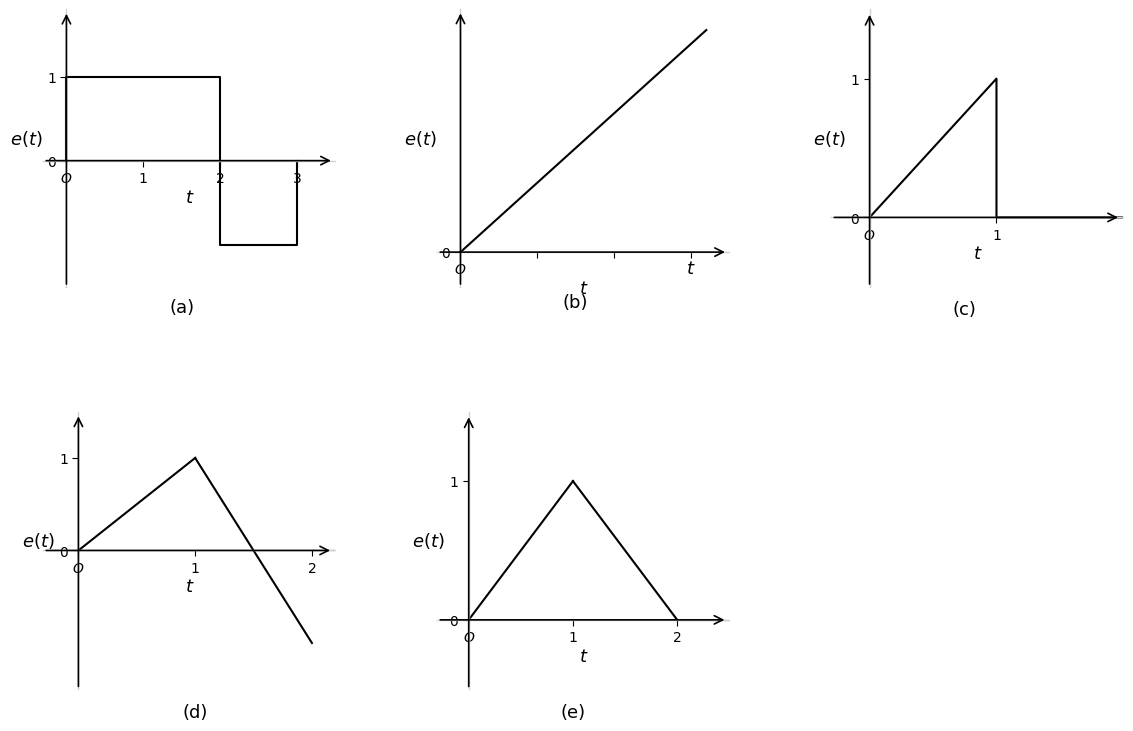
\includegraphics[width=0.5\textwidth]{img/2.21.png}
\caption{题2.21图}
\end{figure}
\end{problem}

\begin{solution}
(a)

由图(a)可得

$$
e(t) = \varepsilon(t) - 2\varepsilon(t-2) + \varepsilon(t-3)
$$

所以
$$
\begin{aligned}
r_{zs} &= h(t) * e(t) = \frac{\mathrm{d}r_\varepsilon(t)}{\mathrm{d}t} * e(t) \\
&= r_\varepsilon(t) * \frac{\mathrm{d}}{\mathrm{d}t}e(t) \\
&= (2e^{-2t} - 1)\varepsilon(t) * \frac{\mathrm{d}}{\mathrm{d}t}\big[\varepsilon(t) - 2\varepsilon(t-2) + \varepsilon(t-3)\big] \\
&= (2e^{-2t} - 1)\varepsilon(t) * \big[\delta(t) - 2\delta(t-2) + \delta(t-3)\big] \\
&= (2e^{-2t} - 1)\varepsilon(t) - 2\big[2e^{-2(t-2)} - 1\big]\varepsilon(t-2) + \big[2e^{-2(t-3)} - 1\big]\varepsilon(t-3)
\end{aligned}
$$

(d)
$$
\begin{aligned}
r_{zs} &= r_\varepsilon(t) * \frac{\mathrm{d}}{\mathrm{d}t}e(t) \\
& = (2e^{-2t} - 1)\varepsilon(t) * \frac{\mathrm{d}}{\mathrm{d}t}\big\{t\big[\varepsilon(t)-\varepsilon(t-1)\big] - (t-1)\big[\varepsilon(t-1)-\varepsilon(t-2)\big]\big\} \\
& = (2e^{-2t} - 1)\varepsilon(t) * \big[\varepsilon(t) - 2\varepsilon(t-1) + \varepsilon(t-2) - \delta(t-1) + \delta(t-2)\big] \\
& = \left[\int_0^t (2e^{-2\tau} - 1)\mathrm{d}\tau\right]\varepsilon(t) * \big[\delta(t) - 2\delta(t-1) + \delta(t-2)\big] - \big[2e^{-2(t-1)} - 1\big]\varepsilon(t-1)+ \big[2e^{-2(t-2)} - 1\big]\varepsilon(t-2) \\
& = \big[1-t-e^{-2t}\big]\varepsilon(t) - 2\big[1-t+1-e^{-2(t-1)}\big]\varepsilon(t-1) + \big[1-t+2-e^{-2(t-2)}\big]\varepsilon(t-2) - \big[2e^{-2(t-1)} - 1\big]\varepsilon(t-1) + \big[2e^{-2(t-2)} - 1\big]\varepsilon(t-2) \\
& = (1-t-e^{-2t})\varepsilon(t) - (3-2t)\varepsilon(t-1) + \big[2-t+e^{-2(t-2)}\big]\varepsilon(t-2)
\end{aligned}
$$
\end{solution}

\subsection{2.23}

\begin{problem}
如图所示电路，其输入电压为单个倒锯齿波，求零状态响应电压$u_L(t)$。

\begin{figure}[H]
\centering
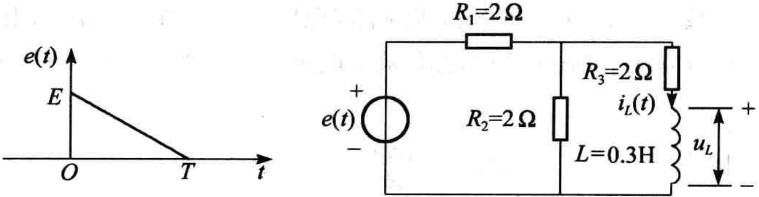
\includegraphics[width=0.5\textwidth]{img/2.23.png}
\caption{题2.23图}
\end{figure}
\end{problem}

\begin{solution}
设电感支路的电流为$i(t)$，方向向下

则由图可列出
$$
u_L(t)+5i_L(t)+2\times\left[i_L(t)+\dfrac{u_L(t)+5i_L(t)}{2}\right]=e(t)
$$
化简得
$$
2u_L(t)+12i_L(t)=e(t)
$$
又因为

$$
u_L(t) = L\dfrac{\mathrm{d}i_L(t)}{\mathrm{d}t} = 0.3\dfrac{\mathrm{d}i_L(t)}{\mathrm{d}t}
$$


所以

$$
2 \times 0.3 \times \dfrac{\mathrm{d}i_L(t)}{\mathrm{d}t} + 12i_L(t) = e(t)
$$


化简得

$$
\dfrac{\mathrm{d}i_L(t)}{\mathrm{d}t} + 20i_L(t) = \dfrac{5}{3}e(t)
$$


所以转移算子

$$
H(p) = \dfrac{\dfrac{5}{3}}{p+20}
$$


所以

$$
h_{i_L}(t) = \dfrac{5}{3}e^{-20t}\varepsilon(t)
$$

$$
h_{u_L}(t) = L\dfrac{\mathrm{d}h_{i_L}(t)}{\mathrm{d}t} = \dfrac{1}{2}\left[-20e^{-20t}\varepsilon(t) + \delta(t)\right]= \dfrac{1}{2}\delta(t) - 10e^{-20t}\varepsilon(t)
$$


零状态响应

$$
\begin{aligned}
u_L(t) &= e(t) * h_{u_L}(t) = e(t) * \left[\frac{1}{2}\delta(t) - 10e^{-20t}\varepsilon(t)\right] \\
&= \frac{e(t)}{2} - 10e^{-20t}\varepsilon(t) * e(t)
\end{aligned}
$$

$$
e(t) = \frac{E}{T}(T-t)\big[\varepsilon(t) - \varepsilon(t-T)\big]
$$

$$
e'(t) = E\delta(t) - \dfrac{E}{T}\big[\varepsilon(t) - \varepsilon(t-T)\big]
$$


所以
$$
\begin{aligned}
u_L(t) &= \frac{E}{2T}(T-t)\big[\varepsilon(t) - \varepsilon(t-T)\big] - 10E\int_0^t e^{-20\tau}\varepsilon(\tau)\mathrm{d}\tau * \left[\delta(t) - \frac{1}{T}\varepsilon(t) + \frac{1}{T}\varepsilon(t-T)\right] \\
&= \frac{E}{2}e^{-20t}\varepsilon(t) - \frac{E}{40T}(1-e^{-20t})\varepsilon(t) + \frac{E}{40T}\left[1-e^{-20(t-T)}\right]\varepsilon(t-T)
\end{aligned}
$$
\end{solution}

\subsection{2.26}

\begin{problem}
已知图电路中，元件参数如下：$R_1 = 1\,\Omega$, $R_2 = 2\,\Omega$, $L_1 = 1\,\mathrm{H}$, $L_2 = 2\,\mathrm{H}$, $M = \dfrac{1}{2}\,\mathrm{H}$, $E = 3\,\mathrm{V}$，设 $t = 0$ 时开关 S 断开，求初级电压 $u_1(t)$ 及次级电流 $i_2(t)$。
\end{problem}

\begin{solution}
开关 S 断开前，电路已达稳态，因为电感电流不能突变，可以求得初次级电流在 $t = 0_-$ 时的起始值，即

$$
i_1(0_-) = i_L(0_-) = \frac{E}{R_1} = 3\,\mathrm{A}
$$

$$
i_2(0_-) = i_{L_2}(0_-) = 0
$$

S 断开时，设 $t = 0$，由KVL得
$$
-M\frac{\mathrm{d}i_1(t)}{\mathrm{d}t} + L_2\frac{\mathrm{d}i_2(t)}{\mathrm{d}t} + R_2 i_2(t) = 0
$$
因为

$$
i_1(t) = 3\varepsilon(-t)
$$

所以

$$
\frac{\mathrm{d}i_1(t)}{\mathrm{d}t} = -3\delta(t)
$$

可得

$$
(p+1)i_2(t) = -\frac{3}{4}\delta(t)
$$

所以冲激响应为

$$
h_{i_2}(t) = -\frac{3}{4}e^{-t}\varepsilon(t)
$$

次级电流 $i_2(t)$ 为

$$
i_2(t) = h_{i_2}(t) = -\frac{3}{4}e^{-t}\varepsilon(t)
$$

初级电压 $u_1(t)$ 为
$$
\begin{aligned}
u_1(t) &= L_1\frac{\mathrm{d}i_1(t)}{\mathrm{d}t} - M\frac{\mathrm{d}i_2(t)}{\mathrm{d}t} \\
&= -3\delta(t) - \frac{1}{2}\left[\frac{3}{4}e^{-t}\varepsilon(t) - \frac{3}{4}\delta(t)\right] \\
&= -\frac{21}{8}\delta(t) - \frac{3}{8}e^{-t}\varepsilon(t)
\end{aligned}
$$
\end{solution}

\section{三角Fourier级数}

当满足Dirichlet条件时，周期为$T$的周期信号$f(t)$可以在区间$ (t_1, t_1+T)$内表示为三角Fourier级数：

$$
\begin{aligned}
f(t) =& \frac{a_0}{2} + a_1 \cos \Omega t + a_2 \cos 2\Omega t + \cdots + a_n \cos n\Omega t + \cdots \\
&+ b_1 \sin \Omega t + b_2 \sin 2\Omega t + \cdots + b_n \sin n\Omega t + \cdots \\
=& \frac{a_0}{2} + \sum_{n=1}^{\infty} \left( a_n \cos n\Omega t + b_n \sin n\Omega t \right)
\end{aligned}
$$

其中 $\Omega = \dfrac{2\pi}{T}$ 为基波频率。

\begin{itemize}
    \item $\dfrac{a_0}{2}$：直流分量
    \item $a_1 \cos \Omega t + b_1 \sin \Omega t$：基波分量
    \item $a_n \cos n\Omega t + b_n \sin n\Omega t \ (n>1)$：n次谐波分量
\end{itemize}

各分量系数

$$
a_0 = \frac{2}{T} \int_{t_1}^{t_1+T} f(t)\,dt
$$

$$
a_n = \frac{2}{T} \int_{t_1}^{t_1+T} f(t) \cos n\Omega t\,dt
$$

$$
b_n = \frac{2}{T} \int_{t_1}^{t_1+T} f(t) \sin n\Omega t\,dt
$$

$$
n = 1,2,3,\cdots
$$

通常取积分限为$(0,T)$或$(-T/2,T/2)$

直流分量
$$
\overline{f(t)} = \frac{1}{T} \int_{t_1}^{t_1+T} f(t)\,dt = \frac{a_0}{2}
$$

\subsection{误差函数}

实际应用中，只能取有限项来进行分析。

有限项Fourier级数：

$$
S_N(t) = \frac{a_0}{2} + \sum_{n=1}^{N} \left( a_n \cos n\Omega t + b_n \sin n\Omega t \right)
$$

误差函数：

$$
\varepsilon_N(t) = f(t) - S_N(t)
$$

均方误差（常用于判定系统性能指标，MSE）：

$$
E_N = \overline{\varepsilon_N^2(t)} = \frac{1}{T} \int_{t_1}^{t_1+T} \varepsilon_N^2(t) \,\mathrm{d}t
$$

$a_0, a_n, b_n$给出最小均方误差意义上的最佳近似。

$$
= \overline{f^2(t)} - \left[ a_0^2 + \frac{1}{2} \sum_{n=1}^{N} \left( a_n^2 + b_n^2 \right) \right]
$$

\subsection{合并同频率项}

两种常用表达式：三角型和余弦型

$$
\begin{aligned}
f(t) &= \frac{A_0}{2} + \sum_{n=1}^{\infty} A_n \cos\left( n\Omega t + \varphi_n \right), \quad t \in \left( t_1, t_1 + T \right) \\
&= \frac{a_0}{2} + \sum_{n=1}^{\infty} \left( a_n \cos n\Omega t + b_n \sin n\Omega t \right)
\end{aligned}
$$

$$
A_0 = a_0
$$

偶函数
$$
A_n = \sqrt{a_n^2 + b_n^2}
$$

奇函数
$$
\varphi_n = -\operatorname{arctg}\frac{b_n}{a_n}
$$

偶函数
$$
a_n = A_n \cos\varphi_n
$$

奇函数
$$
b_n = -A_n \sin\varphi_n
$$

在一定时间间隔内，任意一个代表信号的函数$f(t)$可以用一个直流分量和一系列谐波分量之和来表示。

\subsection{频谱图}

$A_n \sim nΩ$幅度频谱图（通常说频谱指幅度频谱），其中$A_0$为2倍直流分量。

$\varphi_n \sim nΩ$相位频谱图。

周期信号的频谱只出现在$nΩ$等离散频率点，是离散谱。

\subsection{指数Fourier级数}

周期为$T$的周期信号$f(t)$可以在区间$ (t_1, t_1+T)$内用指数Fourier级数表示为：

$$
f(t) = \sum_{n=-\infty}^{\infty} c_n \mathrm{e}^{jn\Omega t}
$$

基波频率
$$
\Omega = \frac{2\pi}{T}
$$

$$
c_n = \frac{1}{T} \int_{t_1}^{t_1+T} f(t) \mathrm{e}^{-jn\Omega t} \,\mathrm{d}t
$$

\subsection{非周期信号的频谱}

非周期信号可看成是$T$趋于无穷大的周期信号。

当周期$T$趋于无穷大时，谱线间隔$\Omega$趋于无穷小，离散频谱趋向于连续频谱。各频率分量的幅度也趋于无穷小，但各分量振幅存在相对差别，且总和仍为一有限值。

为了描述非周期信号的频谱特性，引入频谱密度函数，表示单位频带的频谱值，简称频谱函数$F(jω)$。

\subsubsection{频谱函数}

当$T \rightarrow \infty$，周期信号趋于非周期信号

\begin{itemize}
    \item 复数振幅
    $$
    \dot{A}_n = \frac{2}{T} \int_{-\frac{T}{2}}^{\frac{T}{2}} f(t) \mathrm{e}^{-jn\Omega t} \,\mathrm{d}t \rightarrow 0
    $$
    \item 谱线间隔
    $$
    \Omega = \frac{2\pi}{T} \rightarrow \mathrm{d}\omega \quad \text{无穷小}
    $$
    \item 离散变量
    $$
    n\Omega \rightarrow \omega \quad \text{连续变量}
    $$
\end{itemize}

非周期信号的频谱由周期信号通过极限的方式得到，称为Fourier变换。

定义频谱函数

$$
F(j\omega) = \lim_{T\to\infty} \frac{T\dot{A}_n}{2} = \lim_{\Omega\to 0} \pi \frac{\dot{A}_n}{\Omega}
$$

$$
F(j\omega) = \lim_{T\to\infty} \int_{-\frac{T}{2}}^{\frac{T}{2}} f(t) \mathrm{e}^{-jn\Omega t} \,\mathrm{d}t = \int_{-\infty}^{\infty} f(t) \mathrm{e}^{-j\omega t} \,\mathrm{d}t
$$

\subsubsection{非周期信号的频谱函数举例}

门函数（脉冲宽度为$\tau$）：

$$
G_\tau(t) = \begin{cases} A & -\dfrac{\tau}{2} < t < \dfrac{\tau}{2} \\
0 & t < -\dfrac{\tau}{2} \text{或} t > \dfrac{\tau}{2} \end{cases}
$$

\begin{figure}[H]
\centering
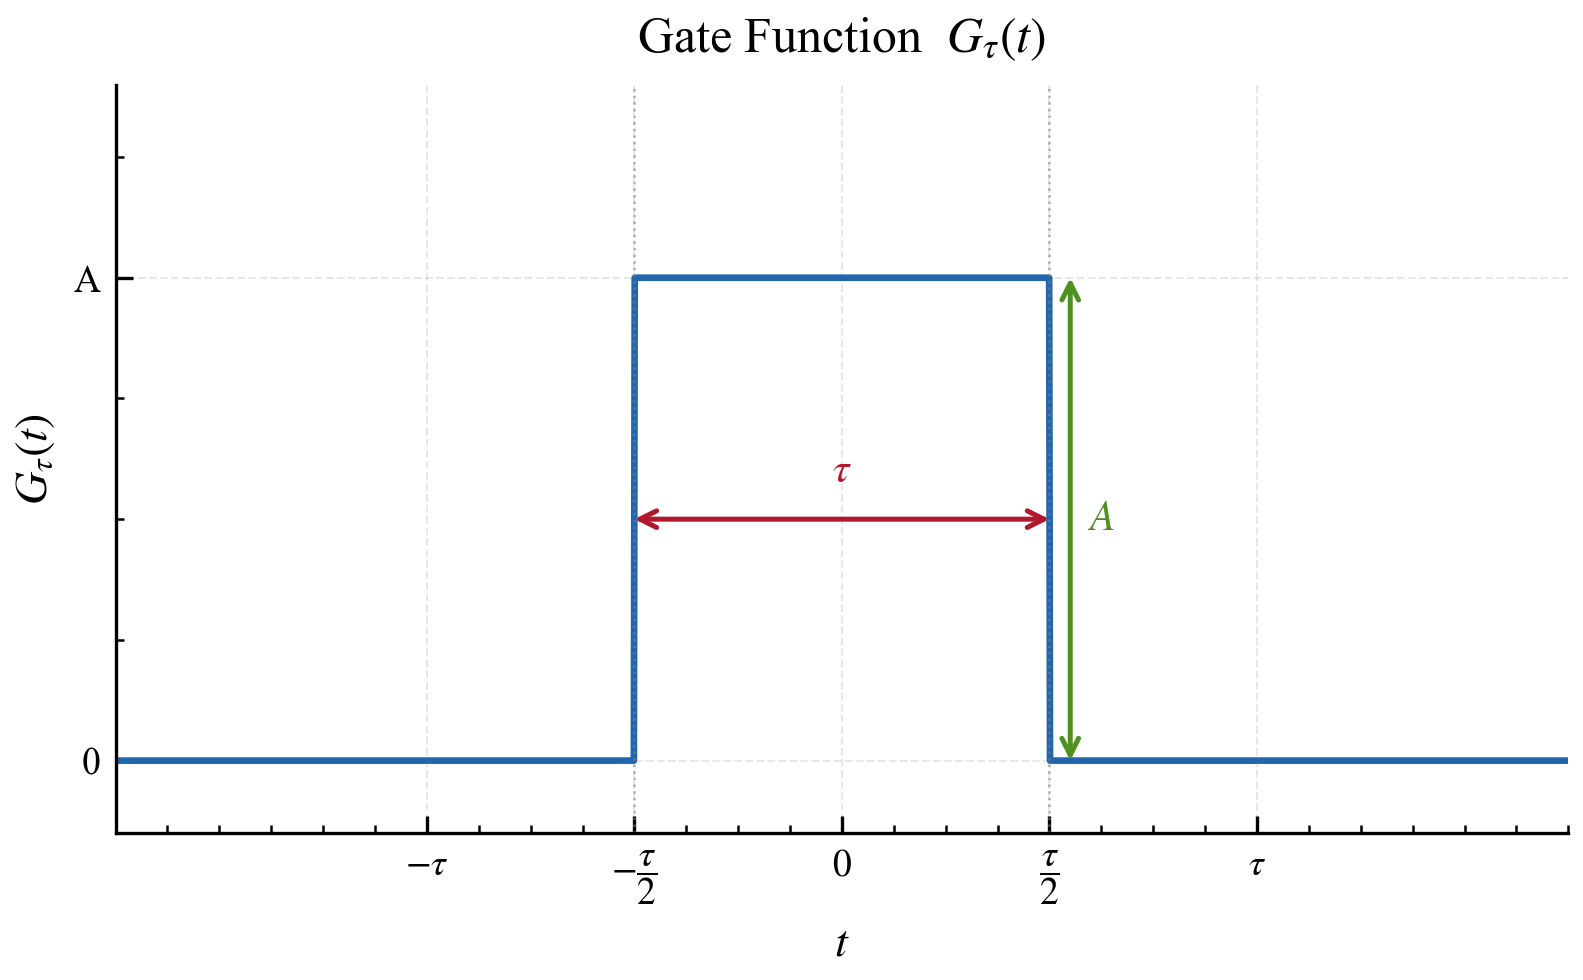
\includegraphics[width=0.5\textwidth]{img/笔记3.1.png}
\caption{门函数波形}
\end{figure}

频谱函数：
$$
\begin{aligned}
F(j\omega) &= \int_{-\infty}^{\infty} f(t) \mathrm{e}^{-j\omega t} \,\mathrm{d}t = A \int_{-\frac{\tau}{2}}^{\frac{\tau}{2}} \mathrm{e}^{-j\omega t} \,\mathrm{d}t \\
&= \frac{A}{-j\omega} \left[ \mathrm{e}^{-j\omega\frac{\tau}{2}} - \mathrm{e}^{j\omega\frac{\tau}{2}} \right] \\
&= \frac{2A}{\omega} \sin\frac{\omega\tau}{2} \\
&= A\tau \,\mathrm{Sa}\left(\frac{\omega\tau}{2}\right)
\end{aligned}
$$

其中

$$
\mathrm{Sa}\left(\frac{\omega\tau}{2}\right) = \frac{\sin(\omega\tau/2)}{\omega\tau/2}
$$

门函数频谱
$$
F(j\omega) = A\tau \,\mathrm{Sa}\left(\frac{\omega\tau}{2}\right)
$$

模量（偶函数）
$$
|F(j\omega)| = A\tau \left| \mathrm{Sa}\left(\frac{\omega\tau}{2}\right) \right|
$$

相位

$$
\varphi(\omega) = \begin{cases} 0 & \dfrac{4n\pi}{\tau} < \omega < \dfrac{4n\pi + 2\pi}{\tau} \\ -\pi & \dfrac{4n\pi + 2\pi}{\tau} < \omega < \dfrac{4n\pi + 4\pi}{\tau} \end{cases}
$$

奇函数，$n = 0, 1, 2, \ldots$

每隔 $\dfrac{2\pi}\tau$ 变换一次

\begin{figure}[H]
\centering
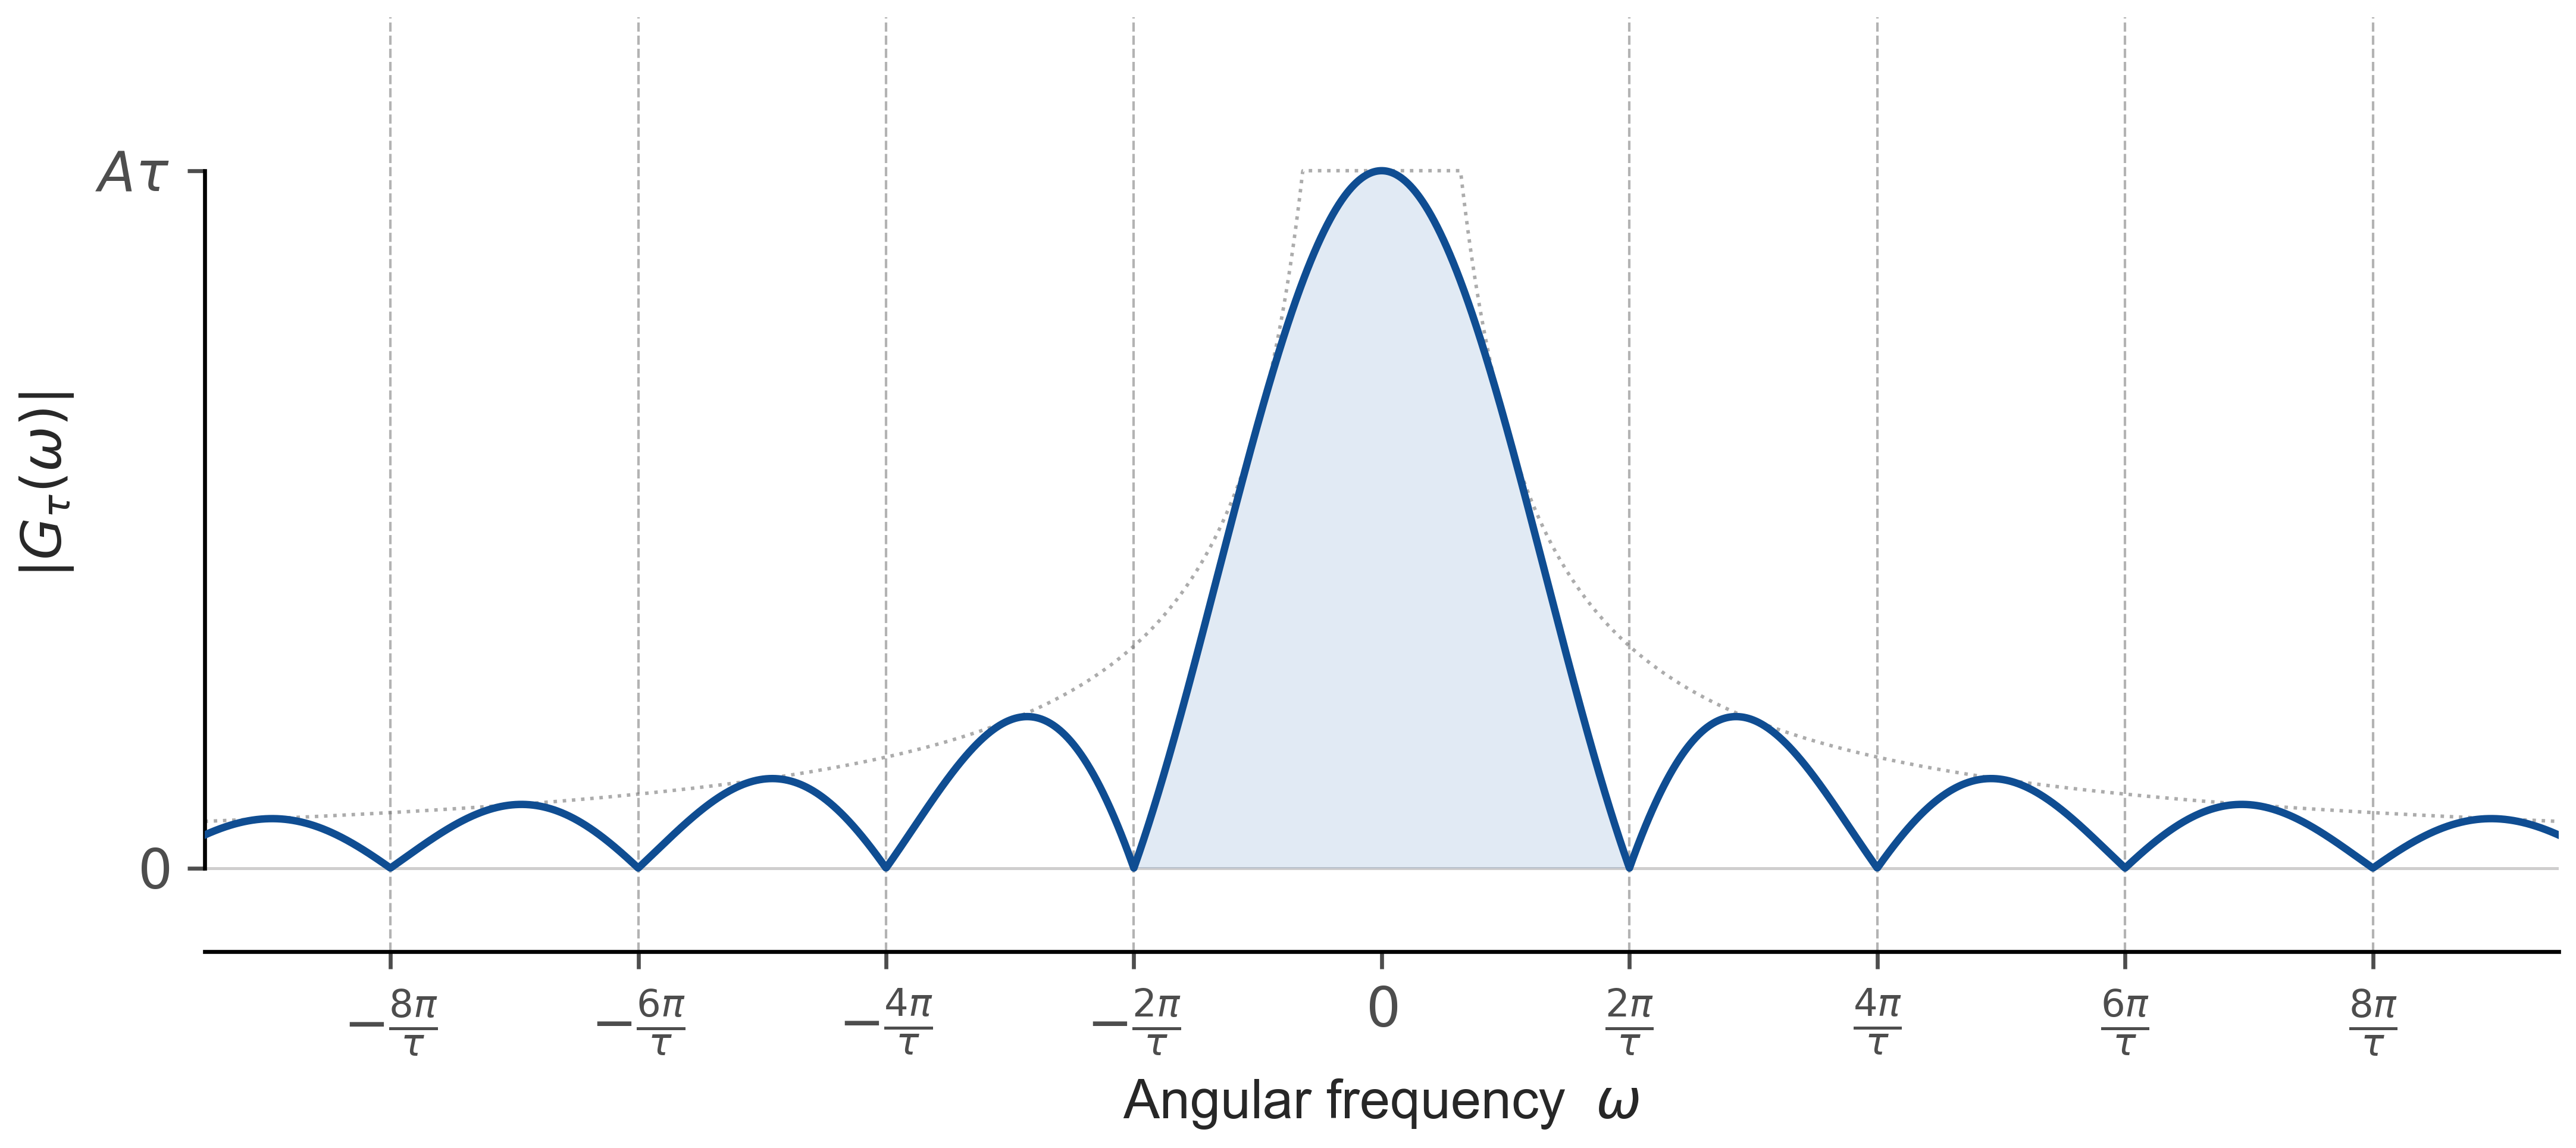
\includegraphics[width=0.5\textwidth]{img/笔记3.2.png}
\caption{门函数频谱}
\end{figure}

\subsection{常用函数的Fourier变换}

$$
F(j\omega)=\mathscr{F}\{f(t)\}=\int_{-\infty}^\infty f(t)\mathrm{e}^{-j\omega t} \mathrm{d}t
$$

$$
f(t)=\mathscr{F}^{-1}\left\{F(j\omega)\right\}=\frac{1}{2\pi}\int_{-\infty}^\infty F(j\omega)\mathrm{e}^{j\omega t}\mathrm{d}\omega
$$

\begin{itemize}
    \item 冲激函数$δ(t)$，$δ’(t)$
    $$
    \delta(t) \leftrightarrow 1
    $$
    
    $$
    \delta^\prime(t) \leftrightarrow j\omega
    $$
    
    \item 常数1
    $$
    1 \leftrightarrow 2\pi\delta(\omega)
    $$
    
    \item 阶跃函数
    $$
    \varepsilon(t) \leftrightarrow \pi\delta(\omega)+\frac{1}{j\omega}
    $$
    
    \item 符号函数
    $$
    \operatorname{sgn}=\begin{cases}-1, &t<0 \\1, &t>0\end{cases} \leftrightarrow \frac{2}{j\omega}
    $$
    \begin{figure}[H]
    \centering
    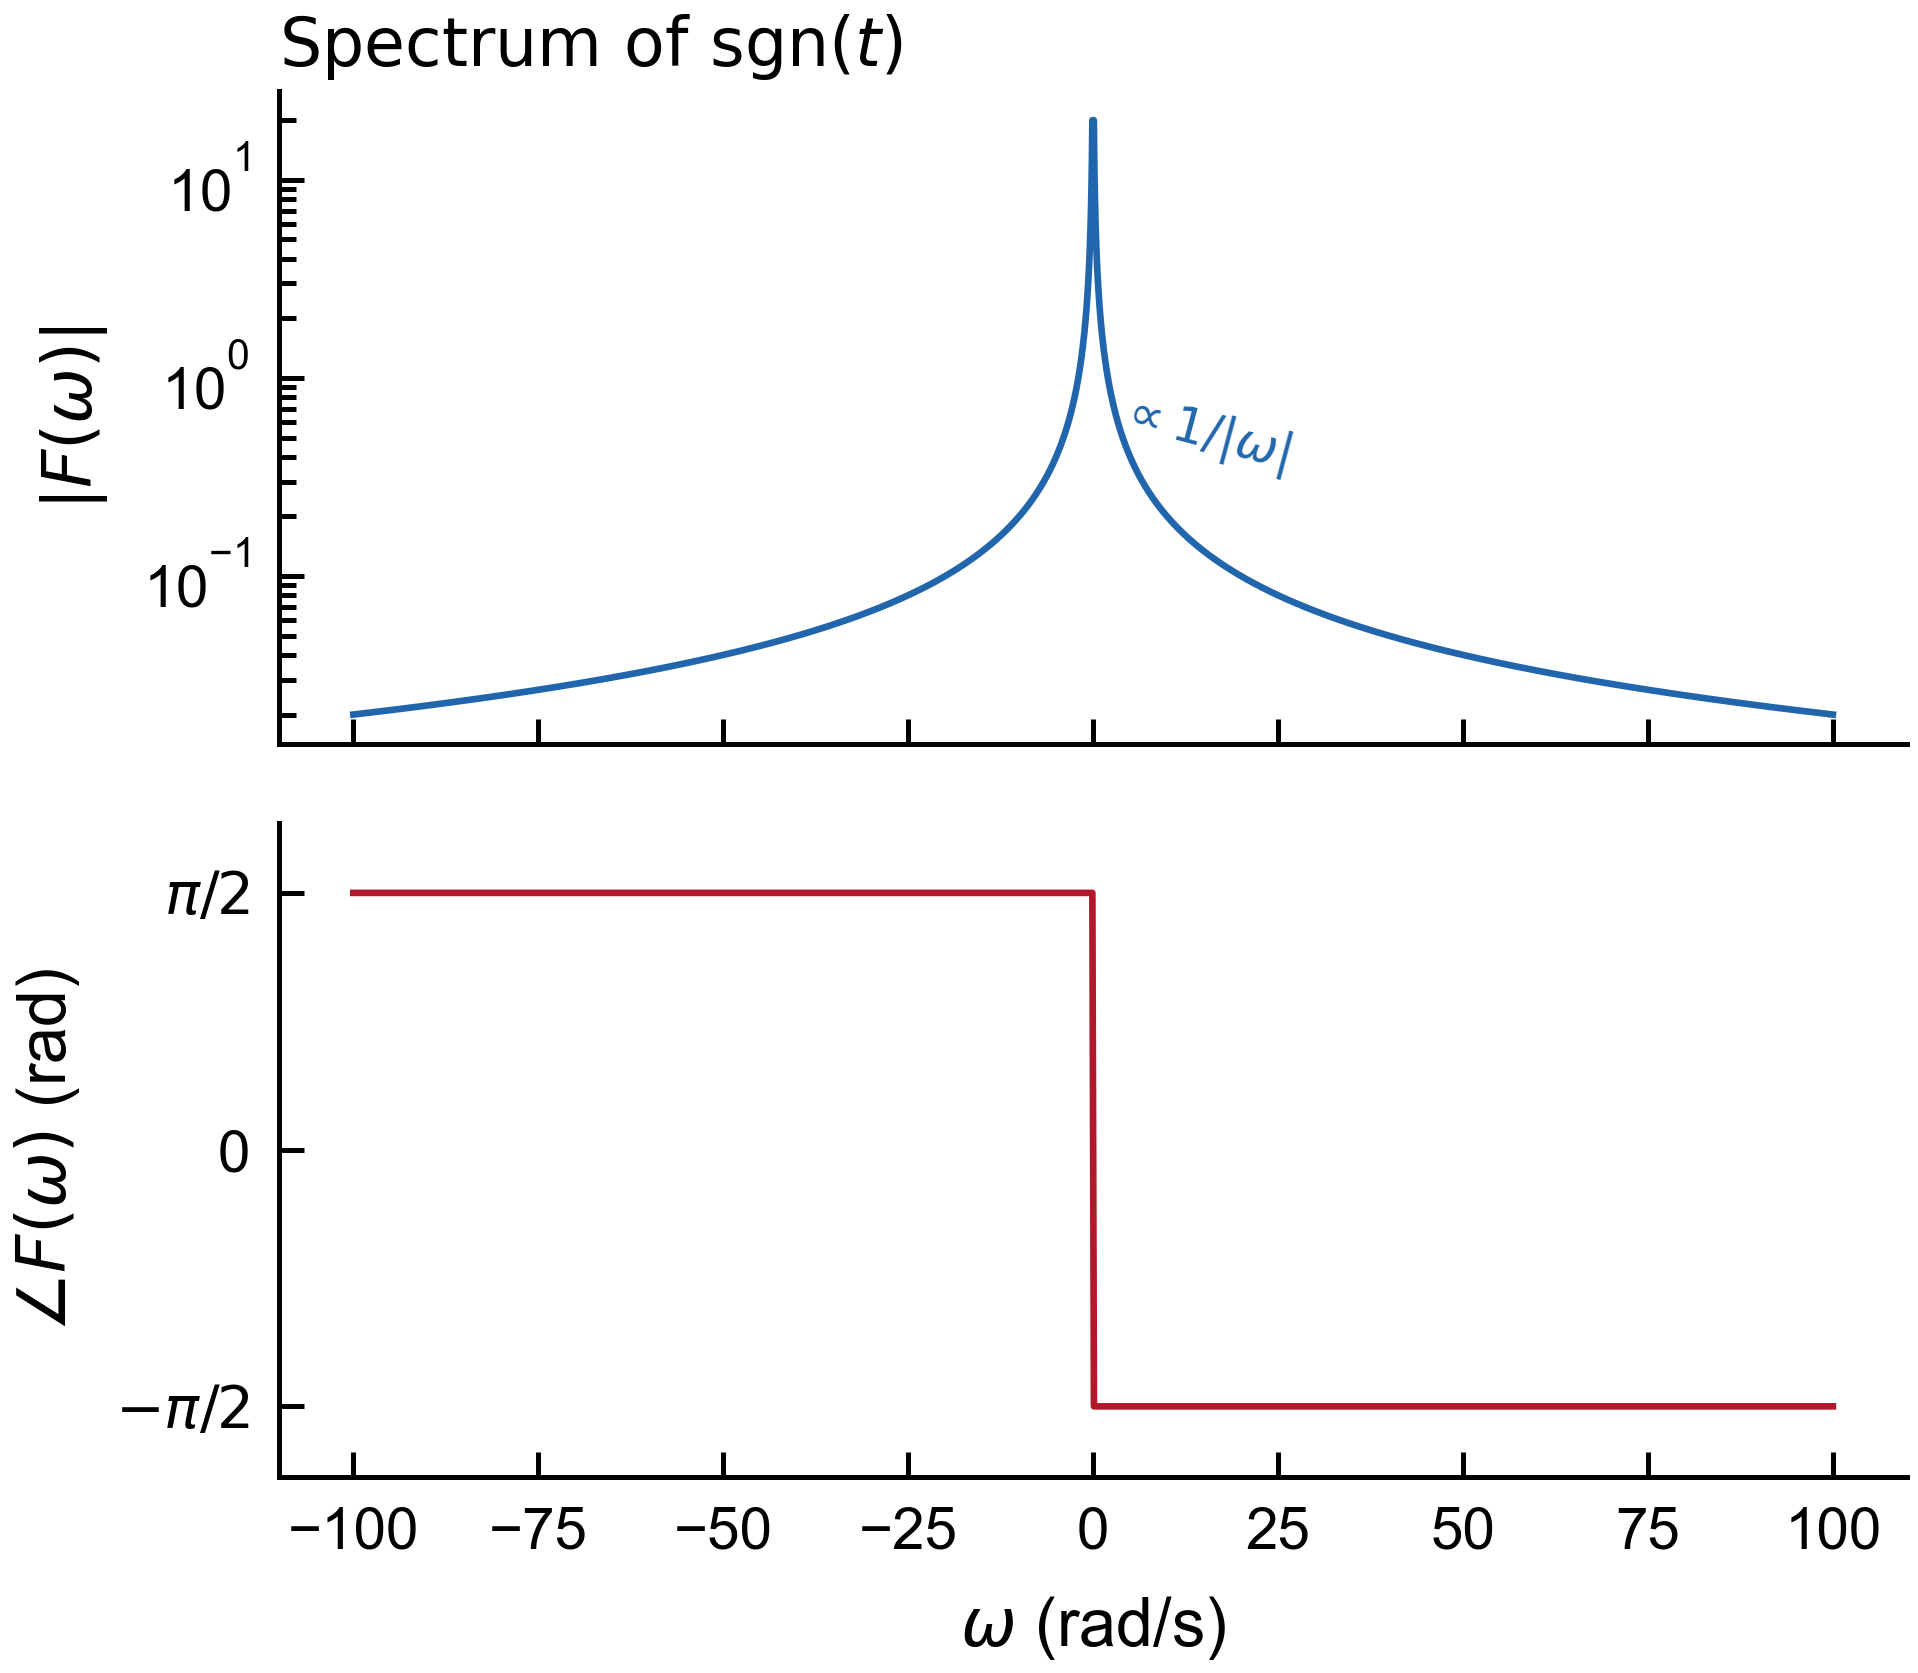
\includegraphics[width=0.5\textwidth]{img/笔记3.3.png}
    \caption{符号函数}
    \end{figure}
    
    \item 门函数
    $$
    G_{\tau}(t)=\begin{cases}A, &|t|<\dfrac{\tau}{2} \\ 0, &|t|>\dfrac{\tau}{2} \end{cases} \leftrightarrow A\tau \operatorname{Sa}\left(\dfrac{\omega\tau}{2}\right)
    $$
    
    \item 三角函数
    $$
    \cos\omega_Ct \leftrightarrow \pi\left[\delta(\omega+\omega_C)+\delta(\omega-\omega_C)\right]
    $$
    
    $$
    \sin\omega_Ct \leftrightarrow j\pi\left[\delta(\omega+\omega_C)-\delta(\omega-\omega_C)\right]
    $$
    
    \item 因果指数信号
    $$
    e^{-at}\varepsilon(t) \leftrightarrow \frac{1}{j\omega+a}
    $$
\end{itemize}

\subsection{Fourier变换的性质}

\subsubsection{线性特性}

\subsubsection{延时特性}

时域延时$t_0$ ，频域相位$ωt_0$
$$
f(t)\leftrightarrow F(j\omega)
$$

$$
f(t-t_0)\leftrightarrow F(j\omega)\mathrm{e}^{-j\omega t_0}
$$

\subsubsection{移频特性}

频域移频$ω_C$，时域乘上$e^{jω_Ct}$
$$
f(t)\leftrightarrow F(j\omega)
$$

$$
f(t)\mathrm{e}^{j\omega t_0}\leftrightarrow F(j(\omega-\omega_C))
$$

推论：
$$
f(t)\cos\omega_C t \longleftrightarrow \frac{1}{2}\Big[F\big(j(\omega+\omega_C)\big)+F\big(j(\omega-\omega_C)\big)\Big]
$$

$$
f(t)\sin\omega_C t \longleftrightarrow \frac{j}{2}\Big[F\big(j(\omega+\omega_C)\big)-F\big(j(\omega-\omega_C)\big)\Big]
$$

\subsubsection{尺度变换特性}

$$
f(t) \leftrightarrow F(j\omega)
$$

$$
f(at) \leftrightarrow \frac{1}{|a|} F\left( j\frac{\omega}{a} \right)
$$

\subsubsection{对称特性}

$$
f(t) \leftrightarrow F(j\omega)
$$

$$
F(jt) \leftrightarrow 2\pi f(-\omega)
$$

\subsubsection{时域微积分特性}

$$
f(t) \leftrightarrow F(j\omega)
$$

时域求导相当于频域乘上因子$jω$。
$$
\frac{\mathrm{d}f(t)}{\mathrm{d}t} \leftrightarrow j\omega F(j\omega)
$$

$$
\frac{\mathrm{d}^n f(t)}{\mathrm{d}t^n} \leftrightarrow (j\omega)^n F(j\omega)
$$

时域积分相当于频域除以因子$jω$。
$$
\int_{-\infty}^tf(\tau)\mathrm{d}\tau \leftrightarrow \frac{1}{j\omega}F(j\omega)
$$

\subsubsection{频域微积分特性}

$$
f(t) \leftrightarrow F(j\omega)
$$

$$
-jtf(t) \leftrightarrow \frac{\mathrm{d}F(j\omega)}{\mathrm{d}\omega}
$$

$$
\pi f(0)\delta(t) + j\frac{f(t)}{t} \leftrightarrow \int_{-\infty}^{\omega} F(j\Omega)\mathrm{d}\Omega
$$

\subsubsection{卷积定理}

$$
f_1(t) \leftrightarrow F_1(j\omega),\quad f_2(t) \leftrightarrow F_2(j\omega)
$$
时域卷积定理：时域的卷积运算相当于频域的乘法运算
$$
f_1(t) * f_2(t) \leftrightarrow F_1(j\omega)F_2(j\omega)
$$
频域卷积定理：频域的卷积运算相当于时域的乘法运算
$$
f_1(t)f_2(t) \leftrightarrow \frac{1}{2\pi}\left[F_1(j\omega)*F_2(j\omega)\right]
$$

\subsection{Parseval定理与能量频谱}

\subsubsection{信号的分类——从能量的角度}

\begin{itemize}
    \item 功率信号：能量无限大，功率有限
    
    典型信号：周期信号
    
    \item 能量信号：能量有限，功率为零
    
    典型信号：非周期单脉冲信号
\end{itemize}

\subsubsection{Parseval定理}

对周期信号，在时域和频域求得的信号功率相等，且功率等于该信号在完备正交函数集中各分量的功率之和。

Fourier级数
\begin{align*} f(t) &= \frac{a_0}{2} + \sum_{n=1}^{N}\left( a_n \cos n\Omega t + b_n \sin n\Omega t \right) \\ &= \frac{1}{2}\sum_{n=-\infty}^{\infty} A_n e^{j\phi_n} e^{jn\Omega t} \end{align*}

时域中的功率
$$
P = \overline{f^2(t)} = \frac{1}{T}\int_{-\frac{T}{2}}^{\frac{T}{2}} \left[f(t)\right]^2 \mathrm{d}t
$$

时域功率等于各谐波分量功率之和：
$$
P = \sum_{n=-\infty}^{\infty}\left( \frac{A_n}{2} \right)^2 = \left( \frac{a_0}{2} \right)^2 + \sum_{n=1}^{\infty}\left( \frac{a_n^2+b_n^2}{2} \right)
$$

对能量信号，在时域中求得的能量等于该信号在频域中求得的能量。

Rayleigh定理
\begin{align*} W &= \int_{-\infty}^{\infty} \left[f(t)\right]^2 \mathrm{d}t \\ &= \frac{1}{2\pi}\int_{-\infty}^{\infty} \left|F(j\omega)\right|^2 \mathrm{d}\omega = \int_{-\infty}^{\infty} \left|F(j2\pi f)\right|^2 \mathrm{d}f \end{align*}

定义能量密度频谱(能谱)函数$G(\omega)$，频带$\mathrm{d}\omega$内的信号能量为$G(\omega)\mathrm{d}\omega$，信号在整个频率范围内的能量为
$$
W = \int_{0}^{\infty} G(\omega)\mathrm{d}\omega,\quad G(\omega) = \frac{1}{\pi}\left|F(j\omega)\right|^2
$$

能谱与幅谱平方的形状相同，与相位频谱无关。

\subsubsection{频带宽度和脉冲宽度}

从能量角度，脉冲宽度 $\tau$ 定义为脉冲中绝大部分能量所集中的那段时间。
$$
\int_{-\frac{\tau}{2}}^{\frac{\tau}{2}} \left[f(t)\right]^2 \mathrm{d}t = \eta W
$$

从能量角度，频带宽度BW定义为脉冲中绝大部分能量所集中的那段频段。
$$
\frac{1}{\pi}\int_{0}^{\mathrm{BW}} \left|F(j\omega)\right|^2 \mathrm{d}\omega = \eta W
$$

\section{例题}

\subsection{例题1}

\begin{problem}
求周期信号的周期$T$，基波频率$\Omega$，并画出频谱图。
$$
f(t)=1-\dfrac{1}{2}\cos\left(\dfrac{\pi}{4}t-\dfrac{2\pi}{3}\right)+\dfrac{1}{4}\sin\left(\dfrac{\pi}{3}t-\dfrac{\pi}{6}\right)
$$
\end{problem}

\begin{solution}
$T_1=8,\quad T_2=6$

周期$T=\operatorname{lcm}(8, 6)=24$，基波频率$Ω=\dfrac{2π}{T}= \dfrac{π}{12}$
$$
\begin{aligned}
f(t) &= \frac{A_0}{2} + \sum_{n=1}^{\infty} A_n \cos\left(n\Omega t + \phi_n\right) \\
&= \frac{2}{2} + \frac{1}{2}\cos\left(3\frac{\pi}{12}t + \frac{\pi}{3}\right) + \frac{1}{4}\cos\left(4\frac{\pi}{12}t - \frac{2\pi}{3}\right) \\
&=\frac{2}{2} + \frac{1}{2}\cos\left(3\frac{\pi}{12}t + \frac{\pi}{3}\right) + \frac{1}{4}\cos\left(4\frac{\pi}{12}t - \frac{2\pi}{3}\right)
\end{aligned}
$$


基波频率
$$
\Omega=\dfrac{\pi}{12}
$$
绘制频谱图：

先看常数项$1$，这是直流分量，也就是频率为 $0$ 的分量。因此在 $\omega=0$ 处有一根谱线，幅度为$1$。

直流项没有振荡，所以相位一般写成 $0$，或者说相位无实际意义。

再看第一项

$$
\frac12\cos\left(3\Omega t+\frac{\pi}{3}\right)
$$

这一项对应：

$$
k=3
$$

$$
\omega=3\Omega=3\cdot \frac{\pi}{12}=\frac{\pi}{4}
$$

幅度为$\dfrac12$，相位为$\dfrac{\pi}{3}$

所以在 $\omega=\dfrac{\pi}{4}$ 处，幅度谱画高度为 $\dfrac12$ 的谱线；相位谱画相位为 $\dfrac{\pi}{3}$ 的谱线。

再看第二项：

$$
\frac14\cos\left(4\Omega t-\frac{2\pi}{3}\right)
$$

于是这一项对应：

$$
k=4
$$

$$
\omega=4\Omega=4\cdot \frac{\pi}{12}=\frac{\pi}{3}
$$

幅度为$\dfrac14$，相位为$-\dfrac{2\pi}{3}$

\begin{figure}[H]
\centering
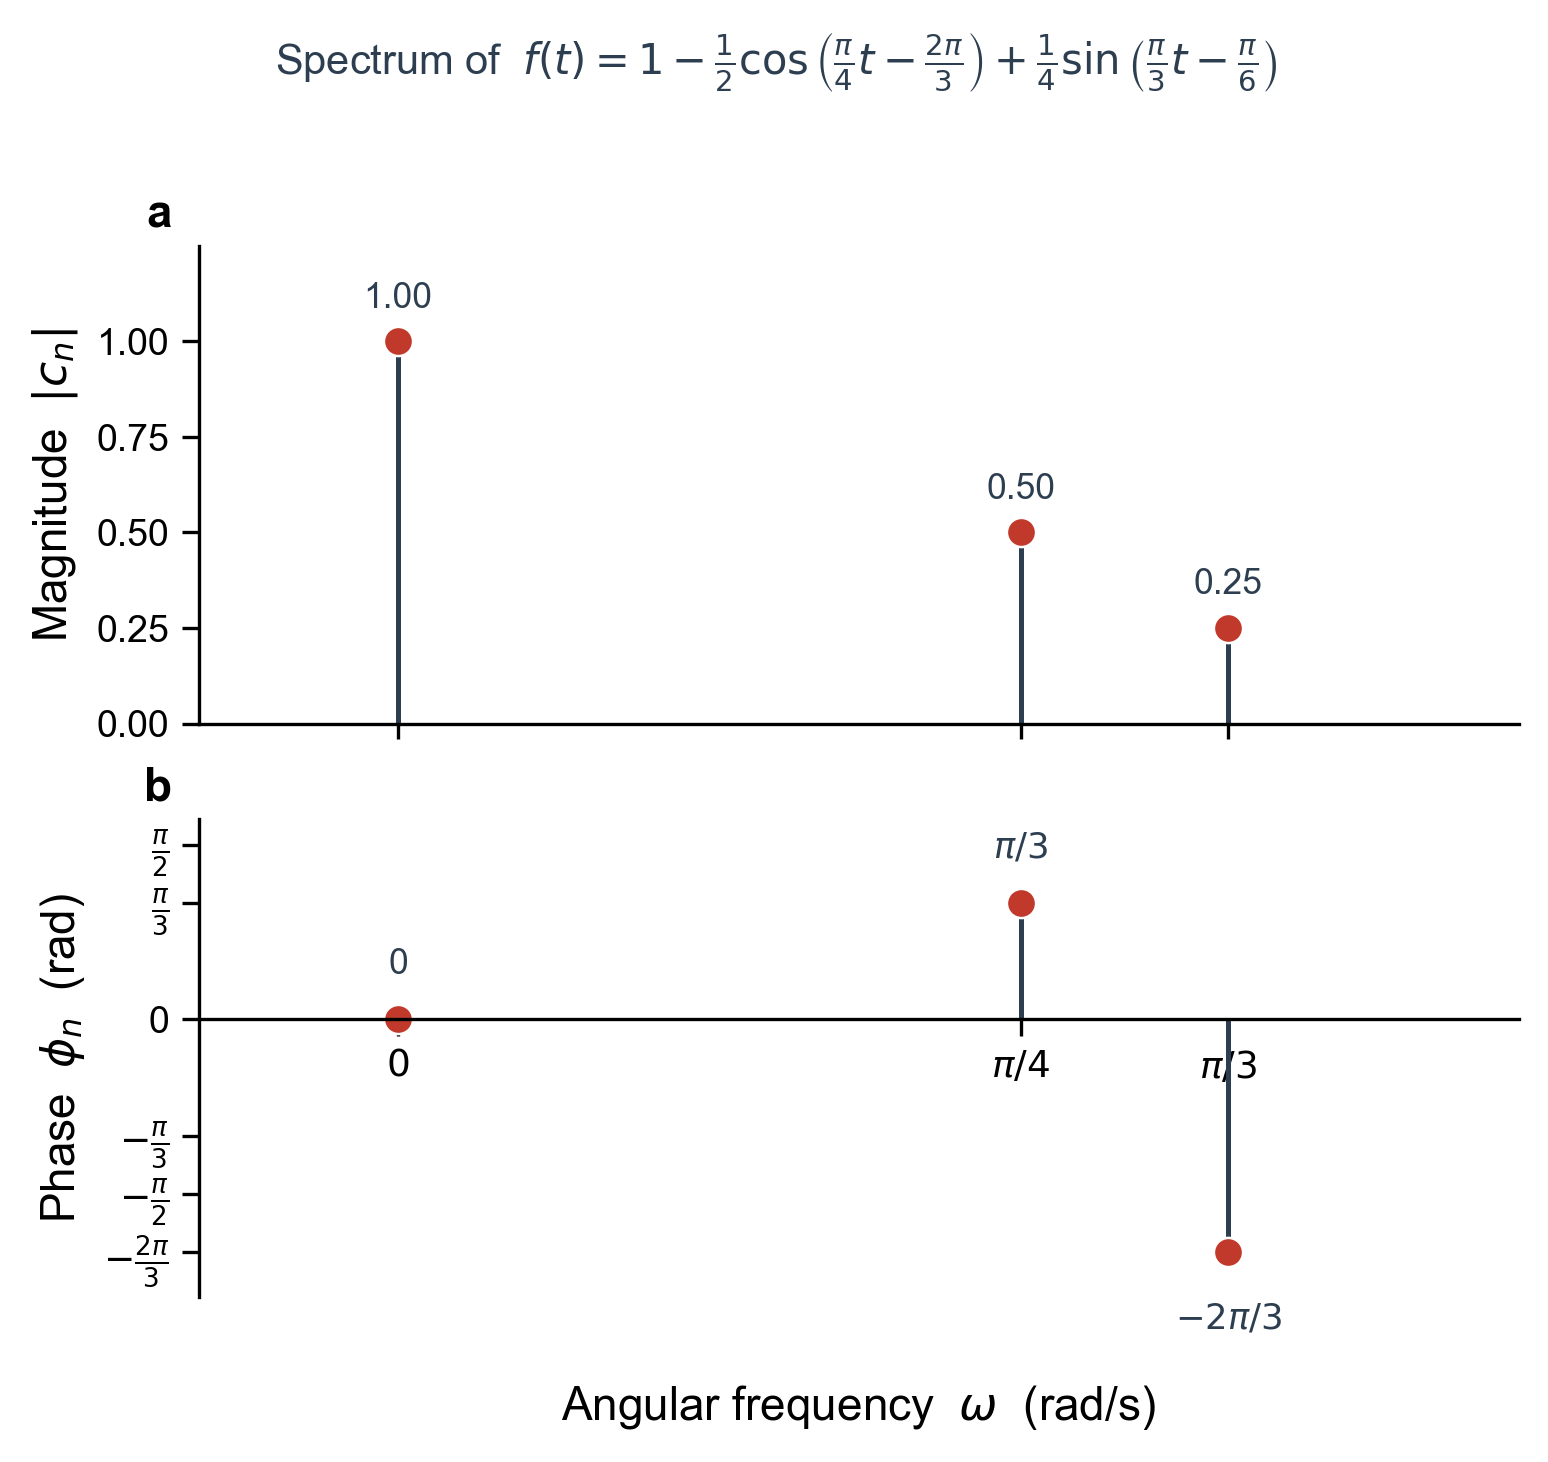
\includegraphics[width=0.5\textwidth]{img/例题1.2.png}
\caption{例题1频谱图}
\end{figure}
\end{solution}

\subsection{例题2}

\begin{problem}
周期脉冲函数的频谱

周期为 $T$ 的矩形脉冲信号 $f(t)$，脉冲幅度为 $A$，脉冲宽度为 $\tau(=-\dfrac{T}{5})$：
$$
f(t) = 
\begin{cases} 
A, & -\dfrac{\tau}{2}<t<\dfrac{\tau}{2} \\[8pt]
0, & -\dfrac{T}{2}<t<-\dfrac{\tau}{2} \quad \& \quad \dfrac{\tau}{2}<t<\dfrac{T}{2}
\end{cases}
$$
\begin{figure}[H]
\centering
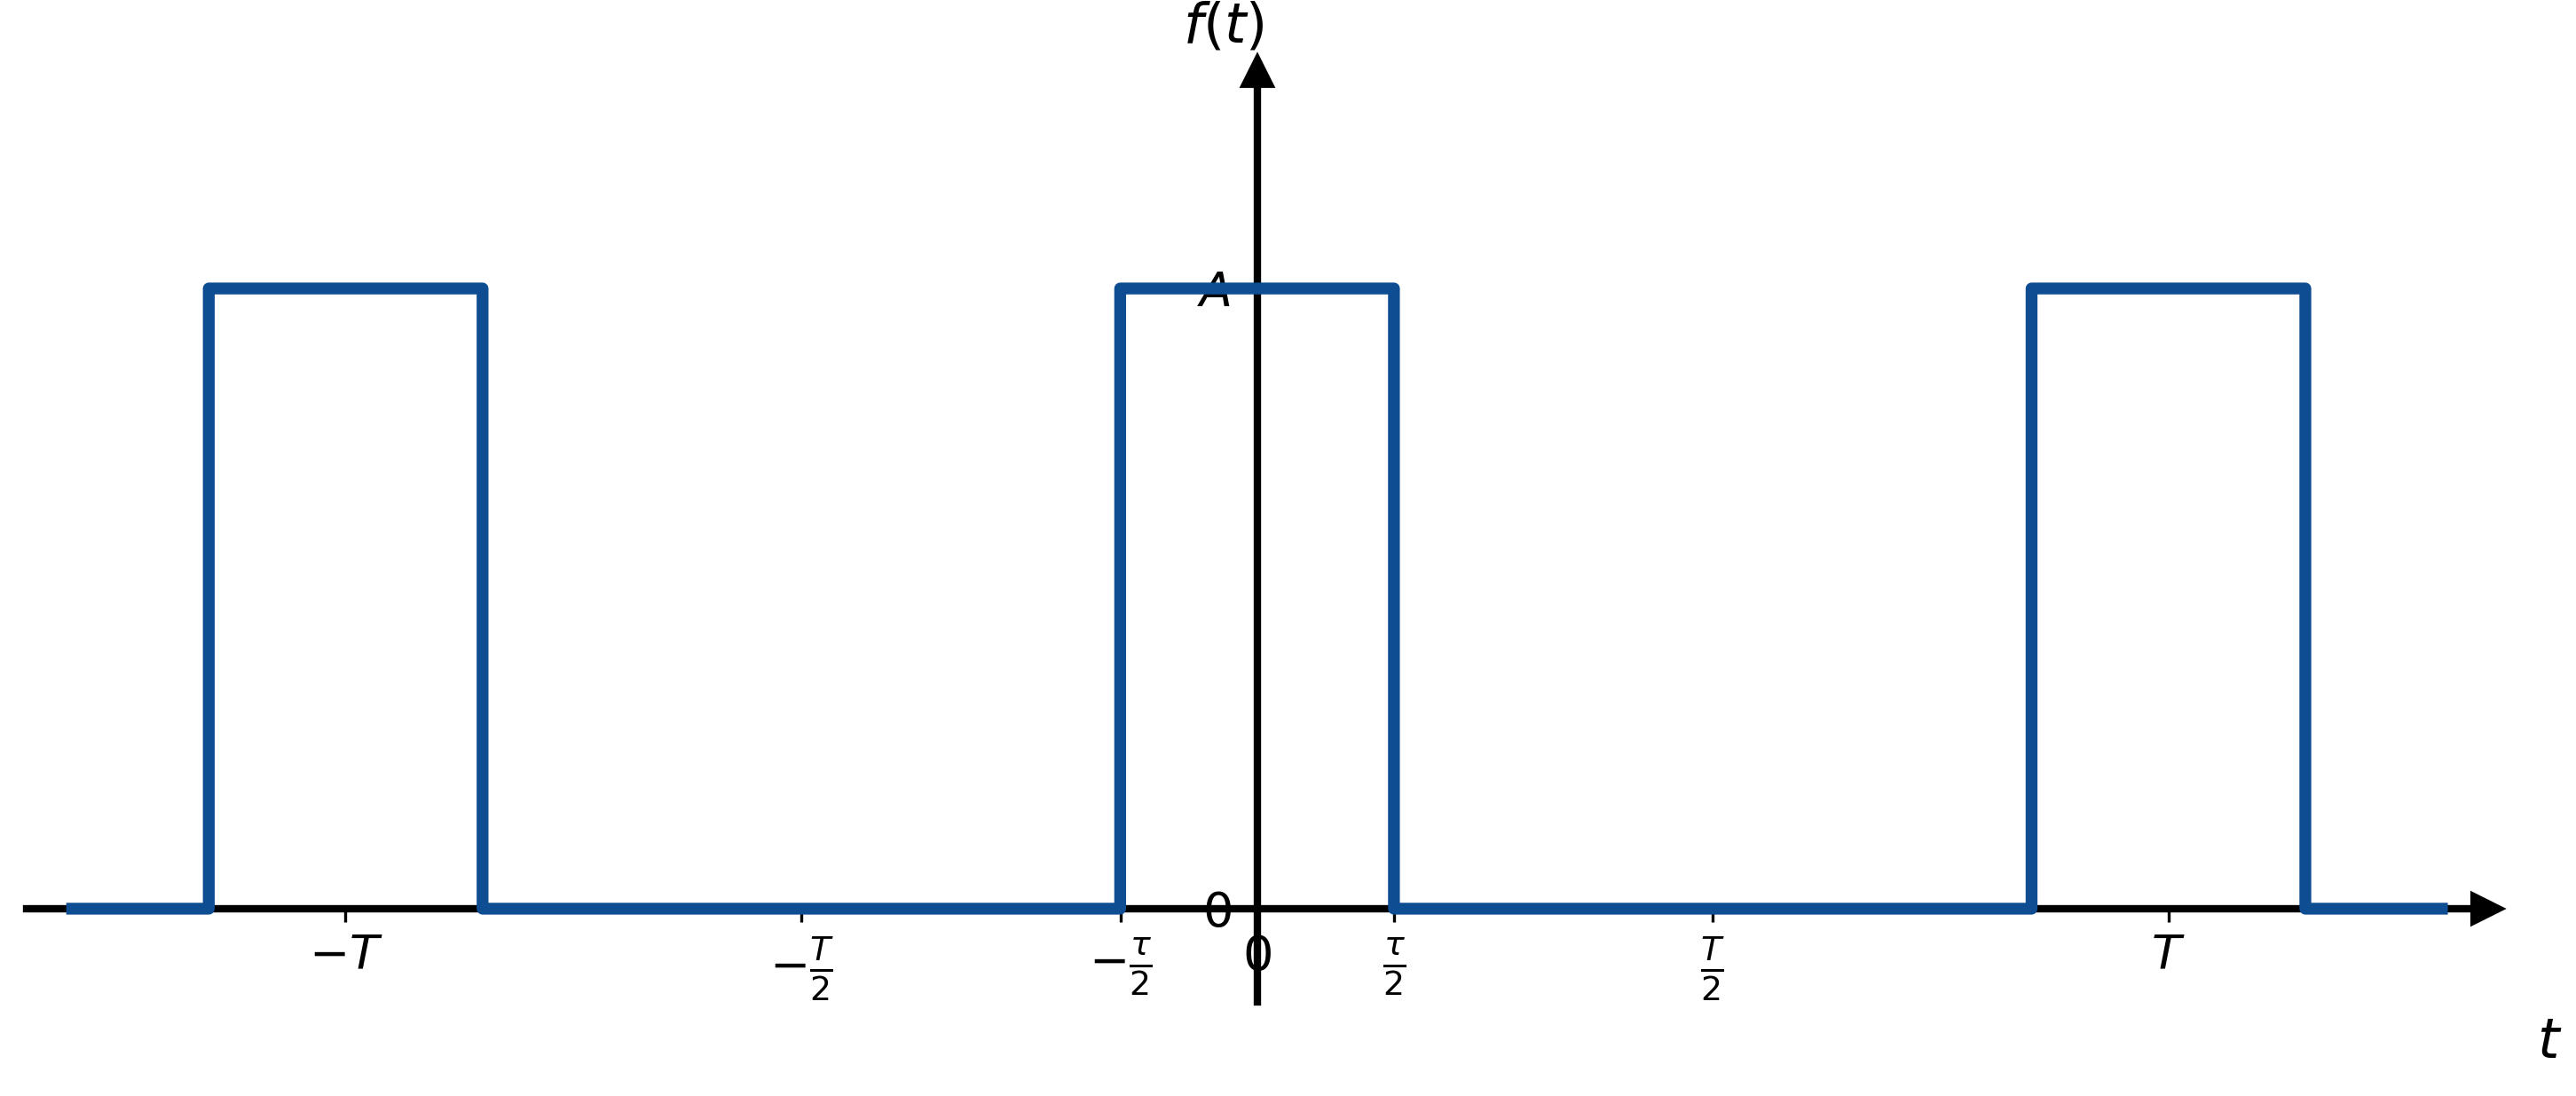
\includegraphics[width=0.5\textwidth]{img/例题3.2.png}
\caption{周期矩形脉冲}
\end{figure}
\end{problem}

\begin{solution}
指数形式傅里叶级数

$$
f(t) = \frac{1}{2} \sum_{n=-\infty}^{+\infty} \dot{A}_n \, e^{jn\Omega t}
$$

其中$\Omega = \dfrac{2\pi}{T}$为基波角频率。

傅里叶系数计算

$$
\begin{aligned}
\dot{A}_n &= \frac{2}{T} \int_{-\dfrac{T}{2}}^{\dfrac{T}{2}} f(t) \, e^{-jn\Omega t} \, dt \\
&= \frac{2}{T} \int_{-\dfrac{\tau}{2}}^{\dfrac{\tau}{2}} A \, e^{-jn\Omega t} \, dt
\end{aligned}
$$

当$n=0$时，
$$
A_0 = \frac{2A\tau}{T}
$$
当$n\neq 0$时，
$$
A_n=\frac{2A}{T}\left[\frac{e^{-jn\Omega t}}{-jn\Omega}\right]_{-\tau/2}^{\tau/2}
$$
代入上下限：
$$
A_n=\frac{2A}{T}\cdot \frac{e^{-\dfrac{jn\Omega \tau}2}-e^{\dfrac{jn\Omega \tau}2}}{-jn\Omega}
$$
利用公式
$$
e^{-jx}-e^{jx}=-2j\sin x
$$
得到
$$
A_n=\frac{2A}{T}\cdot \frac{2\sin(n\Omega\tau/2)}{n\Omega}
$$
即
$$
A_n=\frac{2A\tau}{T}\operatorname{Sa}\left(n\pi\frac{\tau}{T}\right)
$$

因此频谱是在$\omega=n\Omega=n\dfrac{2\pi}{T}$处的一系列离散谱线，谱线高度由
$$
|\dfrac{A_n}2|=\left|
\frac{A\tau}{T}
\operatorname{Sa}
\left(n\pi\frac{\tau}{T}\right)
\right|
$$
决定。

\begin{table}[H]
\centering
\begin{tabular}{c|c}
\hline
$\omega$ & $\|\dfrac{A_n}2\|$ \\
\hline
$0$ & $\dfrac{A\tau}{T}$ \\
\hline
$\pm\Omega$ & $\left\|\dfrac{A\tau}{T}\operatorname{Sa}\left(\pi\frac{\tau}{T}\right)\right\|$ \\
\hline
$\pm 2\Omega$ & $\left\|\dfrac{A\tau}{T}\operatorname{Sa}\left(2\pi\frac{\tau}{T}\right)\right\|$ \\
\hline
$\pm 3\Omega$ & $\left\|\dfrac{A\tau}{T}\operatorname{Sa}\left(3\pi\frac{\tau}{T}\right)\right\|$ \\
\hline
$\vdots$ & $\vdots$ \\
\hline
\end{tabular}
\end{table}

$$
\varphi_n=\operatorname{arg}\left(\frac{A_n}{2}\right)
$$

对于这个以 $t=0$ 为中心的周期矩形脉冲，因为它是偶函数，所以复傅里叶系数 $\dfrac{A_n}{2}$ 是\textbf{实数}：

故
$$
\varphi_n=
\begin{cases}
0, &A_n>0 \\
\pi, &A_n<0
\end{cases}
$$

\begin{figure}[H]
\centering
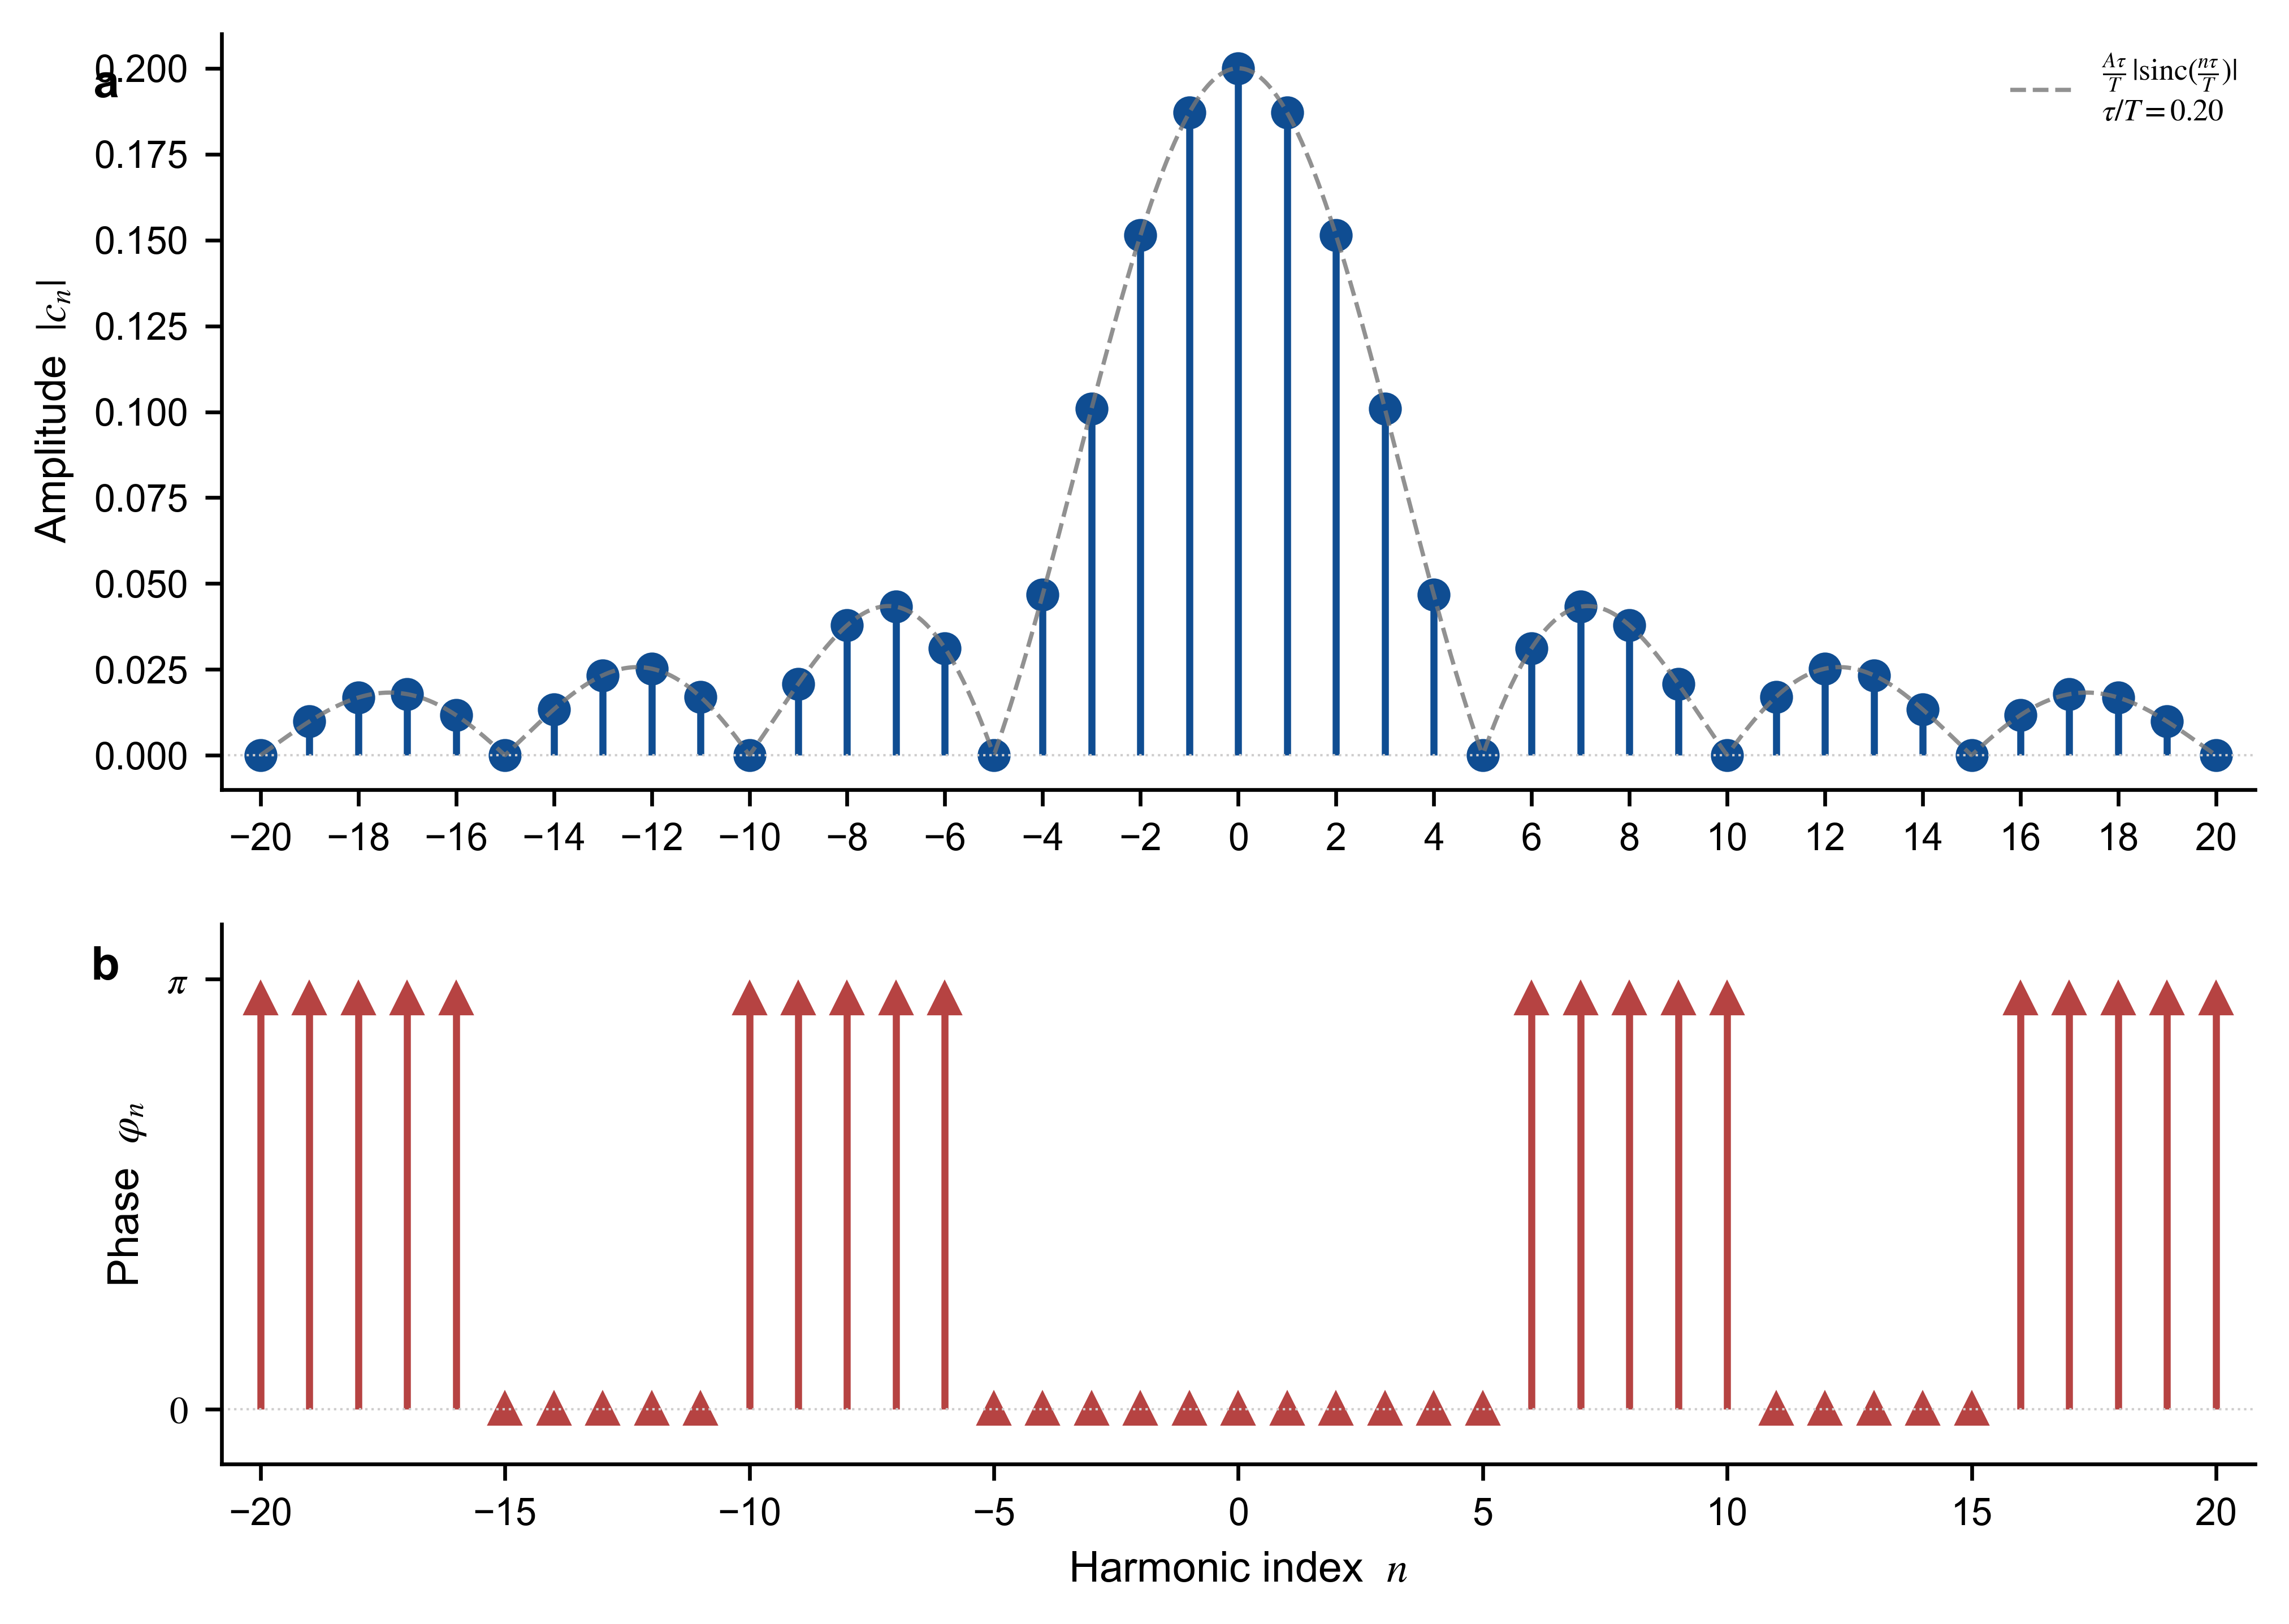
\includegraphics[width=0.5\textwidth]{img/例题3.2.2.png}
\caption{例题2频谱图}
\end{figure}
\end{solution}

\subsection{例题3}

\begin{problem}
求均匀冲激序列的Fourier变换

$$
\delta_T(t) = \delta(t) + \delta(t \pm T) + \delta(t \pm 2T) + \cdots
$$
(周期为$T$)

$$
\delta_T(t) \longleftrightarrow \Omega\delta_\Omega(\omega)
$$
\end{problem}

\begin{solution}
$$
\dot{A}_n = \frac{2}{T} \int_{-\frac{T}{2}}^{\frac{T}{2}} f(t) \mathrm{e}^{-jn\Omega t} \,\mathrm{d}t = \frac{2}{T} \int_{-\frac{T}{2}}^{\frac{T}{2}} \delta(t) \mathrm{e}^{-jn\Omega t} \,\mathrm{d}t = \frac{2}{T}, \quad \Omega = \frac{2\pi}{T}
$$

$$
F(j\omega) = \pi \sum_{n=-\infty}^{\infty} \dot{A}_n \delta(\omega - n\Omega) = \frac{2\pi}{T} \sum_{n=-\infty}^{\infty} \delta(\omega - n\Omega) = \Omega\delta_\Omega(\omega)
$$

冲激序列的Fourier变换仍是冲激序列。
\end{solution}

\subsection{例题4}

\begin{problem}
求矩形调幅信号的Fourier变换
信号表达式：
$$
f(t) = G_\tau(t)\cos \omega_0 t
$$
\begin{figure}[H]
\centering
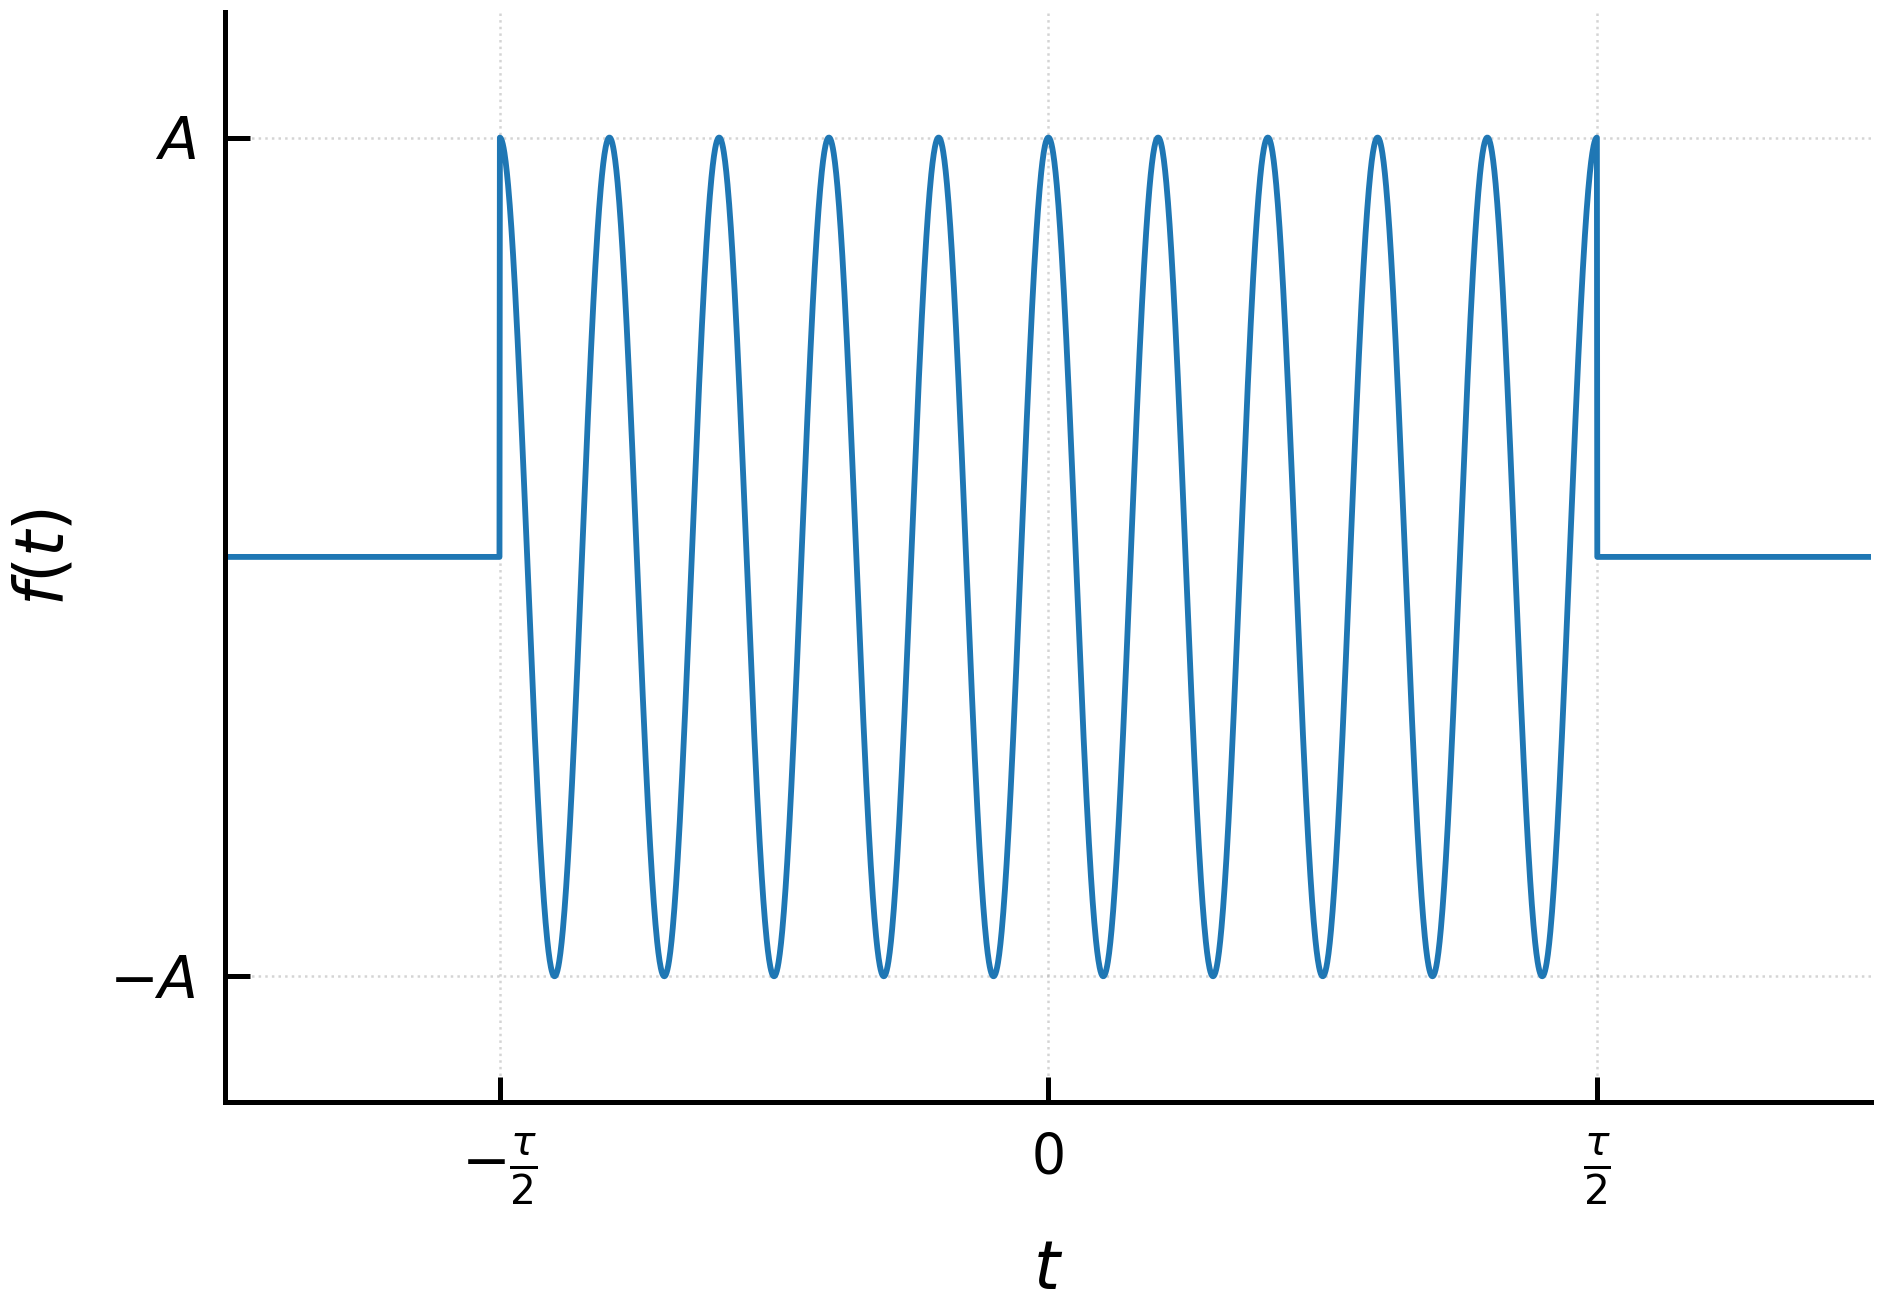
\includegraphics[width=0.5\textwidth]{img/例题3.4.png}
\caption{矩形调幅信号}
\end{figure}
\end{problem}

\begin{solution}
门函数的傅里叶变换对：
$$
G_\tau(t) \leftrightarrow \tau \mathrm{Sa}\left( \frac{\omega \tau}{2} \right)
$$

移频特性及其推论
设 $f(t) \leftrightarrow F(j\omega)$，则
$$
f(t)e^{j\omega_C t} \leftrightarrow F\left( j(\omega-\omega_C) \right)
$$
$$
f(t)\cos \omega_C t \leftrightarrow \frac{1}{2}\left[ F\left( j(\omega+\omega_C) \right)+F\left( j(\omega-\omega_C) \right) \right]
$$

代入频谱得到最终结果：
$$
F(j\omega) = \frac{A\tau}{2}\left[ \mathrm{Sa}\left( \frac{\tau}{2}(\omega+\omega_0) \right)+\mathrm{Sa}\left( \frac{\tau}{2}(\omega-\omega_0) \right) \right]
$$
\end{solution}

\subsection{例题5}

\begin{problem}
求图示梯形脉冲的频谱

\begin{figure}[H]
\centering
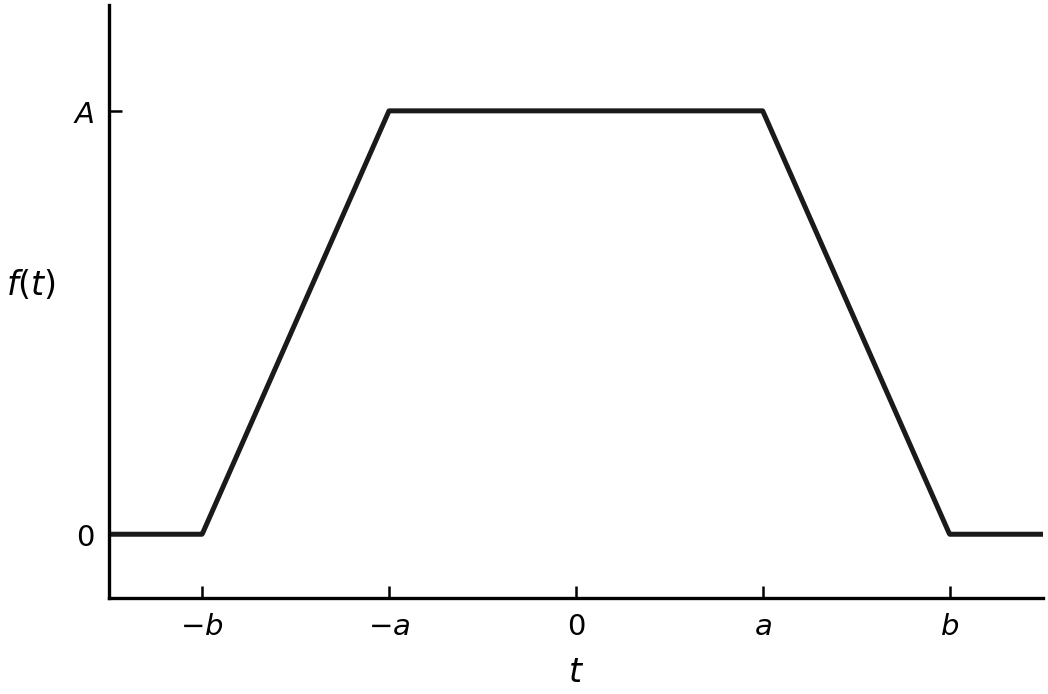
\includegraphics[width=0.5\textwidth]{img/例题3.5.png}
\caption{梯形脉冲}
\end{figure}
\end{problem}

\begin{solution}
对信号做二阶时域微分：
$$
\frac{\mathrm{d}^2 f(t)}{\mathrm{d}t^2} = \frac{A}{b-a}\left[\delta(t+b)-\delta(t+a)-\delta(t-a)+\delta(t-b)\right]
$$

对等式两侧同时取傅里叶变换，由时域微分特性可得：
$$
(j\omega)^2 F(j\omega) = \frac{A}{b-a}\left[e^{j\omega b}-e^{j\omega a}-e^{-j\omega a}+e^{-j\omega b}\right]
$$

\begin{figure}[H]
\centering
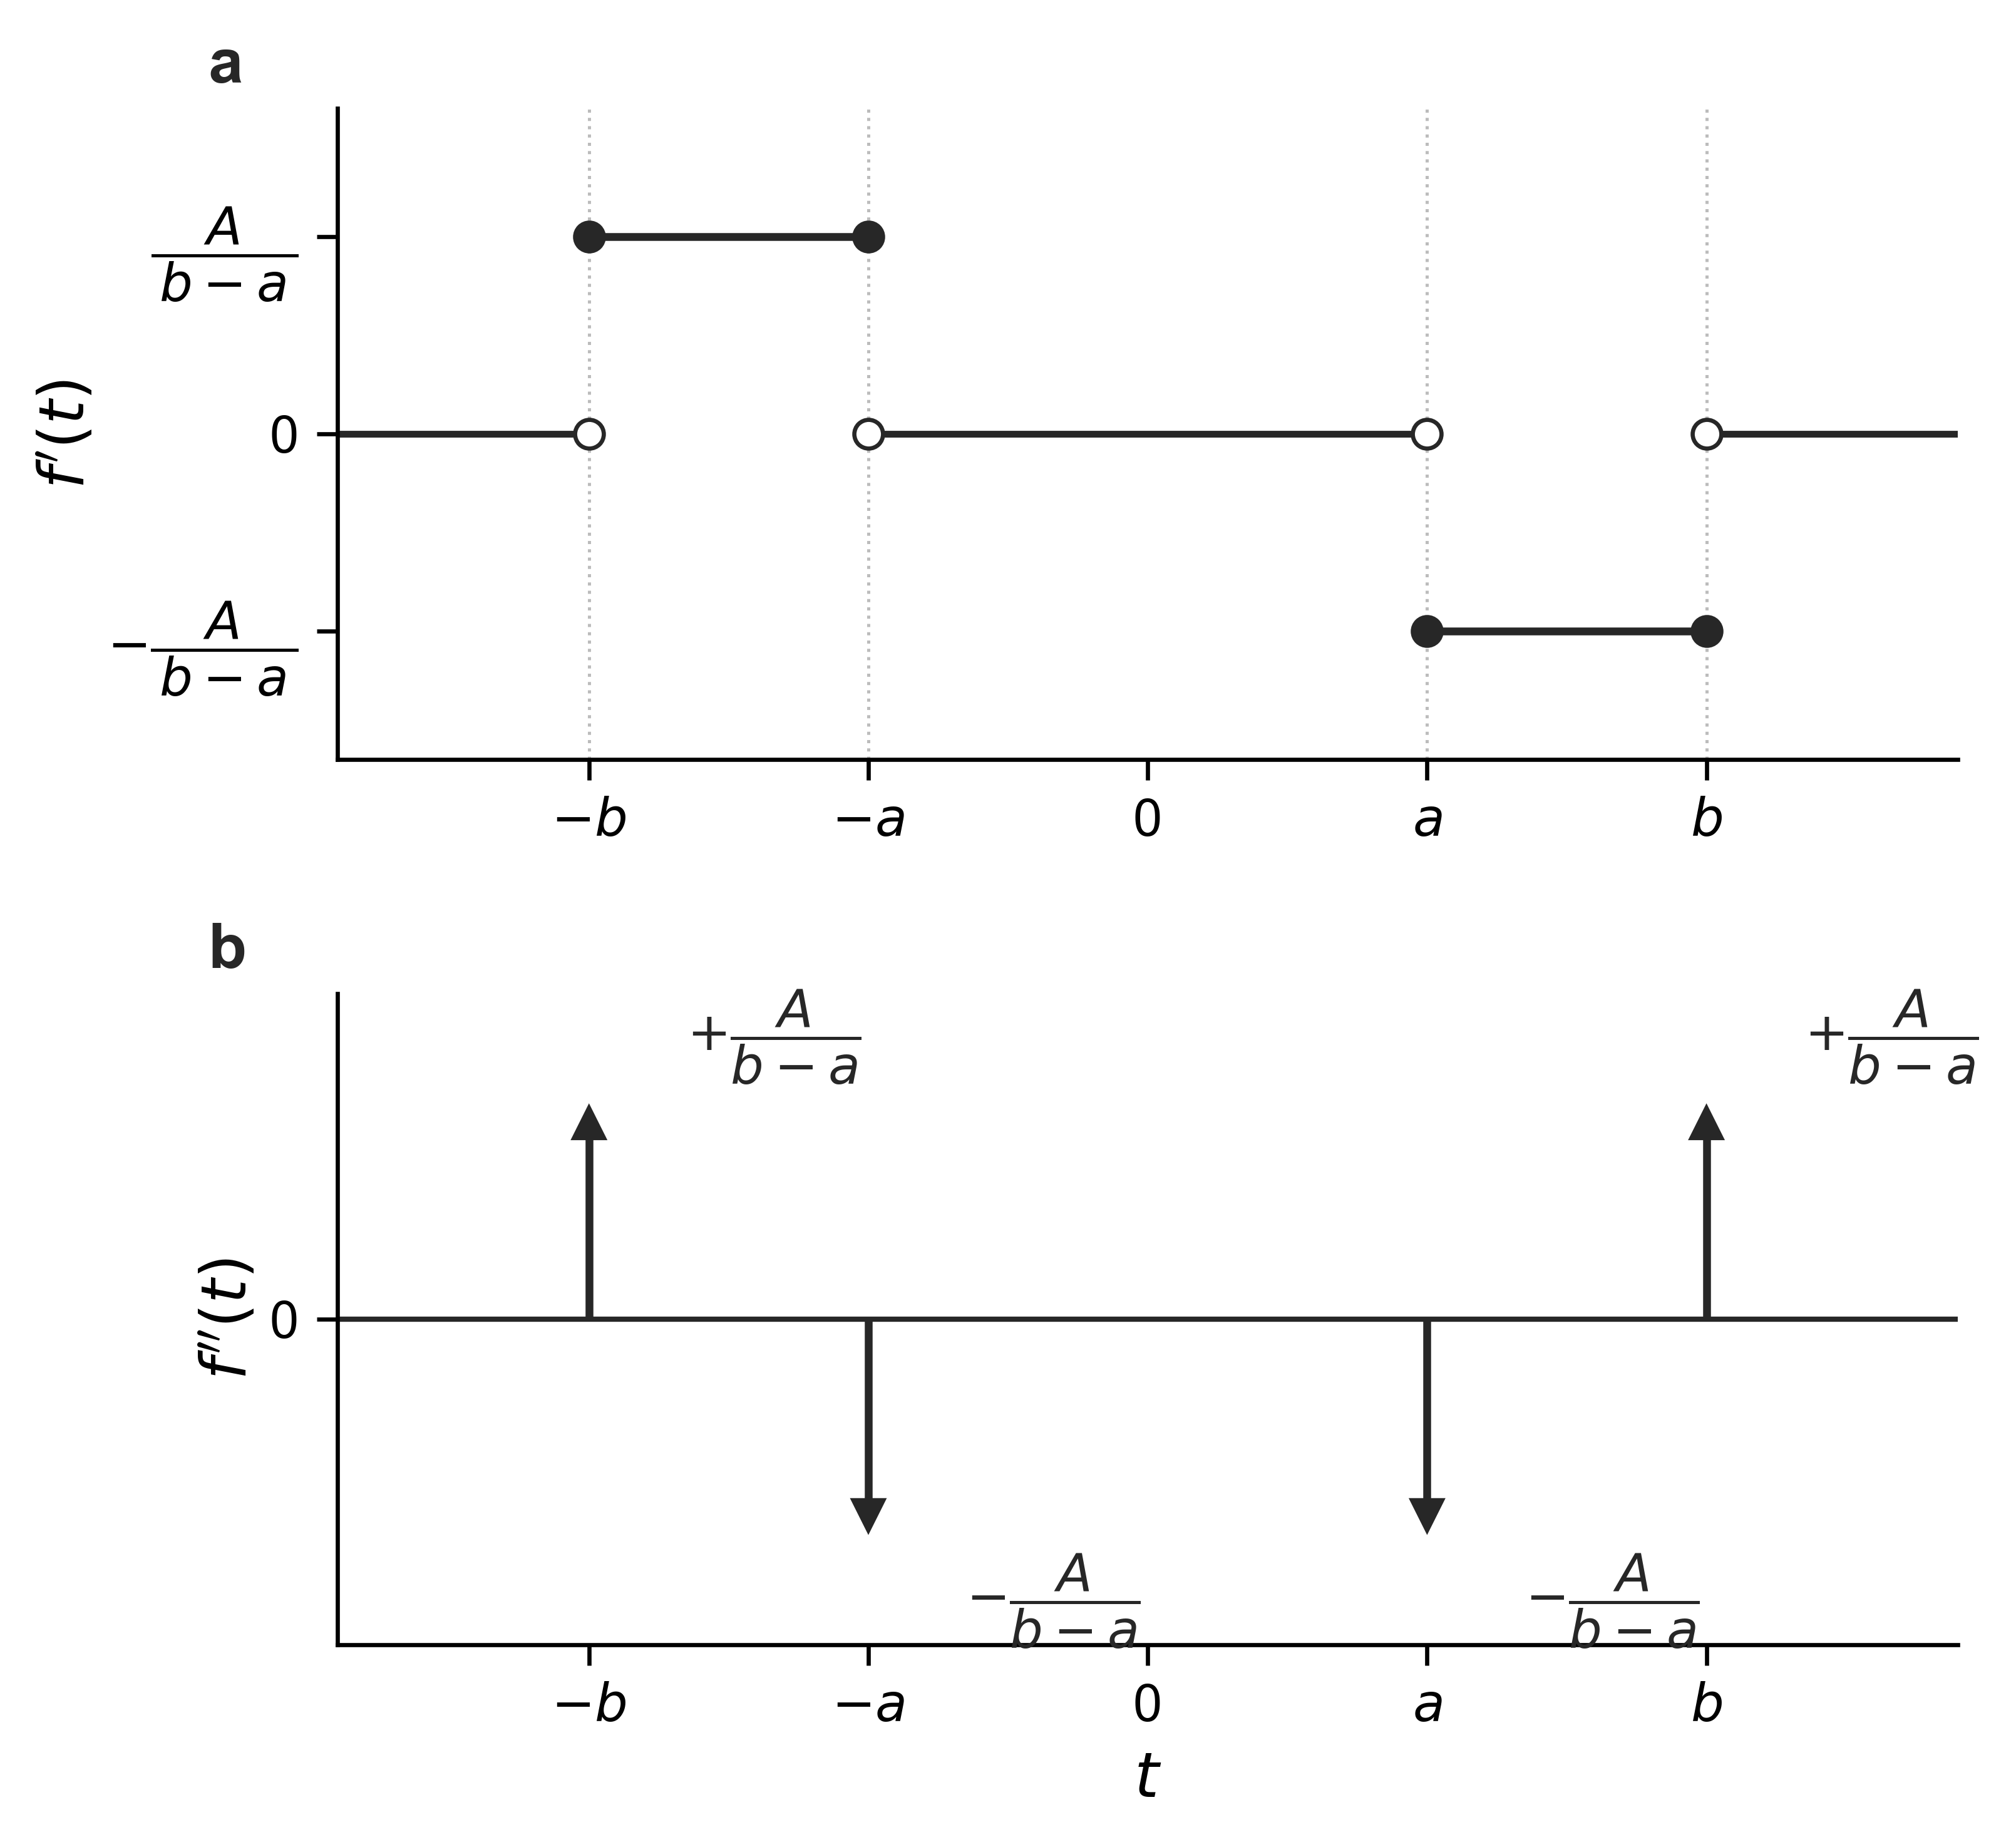
\includegraphics[width=0.5\textwidth]{img/例题3.5.2.png}
\caption{梯形脉冲频谱}
\end{figure}

整理得
$$
F(j\omega)=\frac{2A}{b-a}\left[\frac{\cos b\omega-\cos a\omega}{\omega^2}\right]
$$
\end{solution}

\subsection{3.6}

\begin{problem}
利用周期性矩形脉冲与周期性三角脉冲的傅里叶级数展开式，求如图波形所示信号的傅里叶级数。

\begin{figure}[H]
\centering
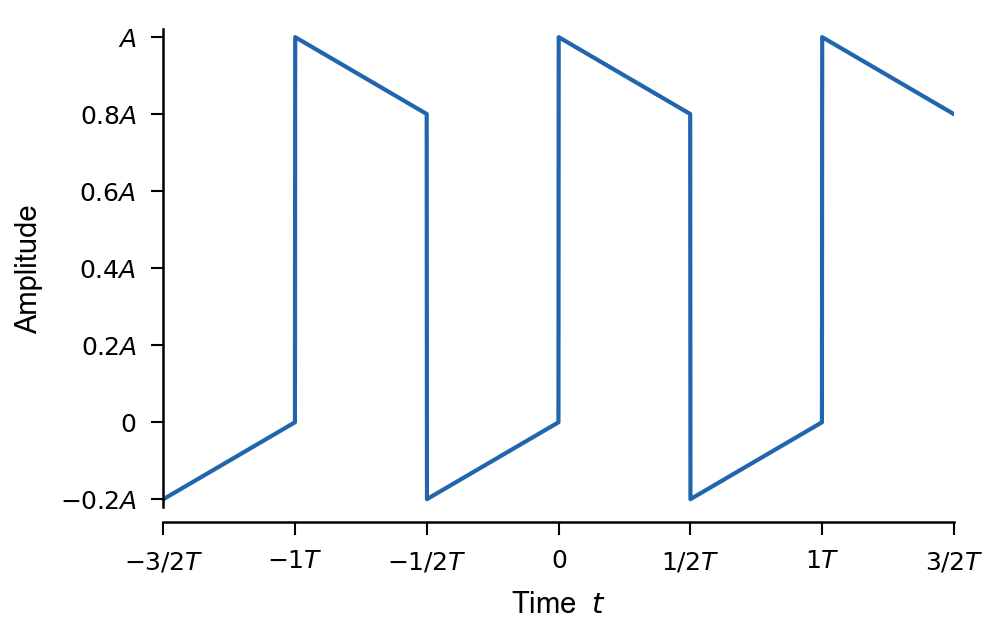
\includegraphics[width=0.5\textwidth]{img/3.6.png}
\caption{题3.6图}
\end{figure}
\end{problem}

\begin{solution}
$f(t)$可看作是一个周期性矩形脉冲$f_1(t)$和一个周期性三角脉冲$f_2(t)$之差（如图所示）

\begin{figure}[H]
\centering
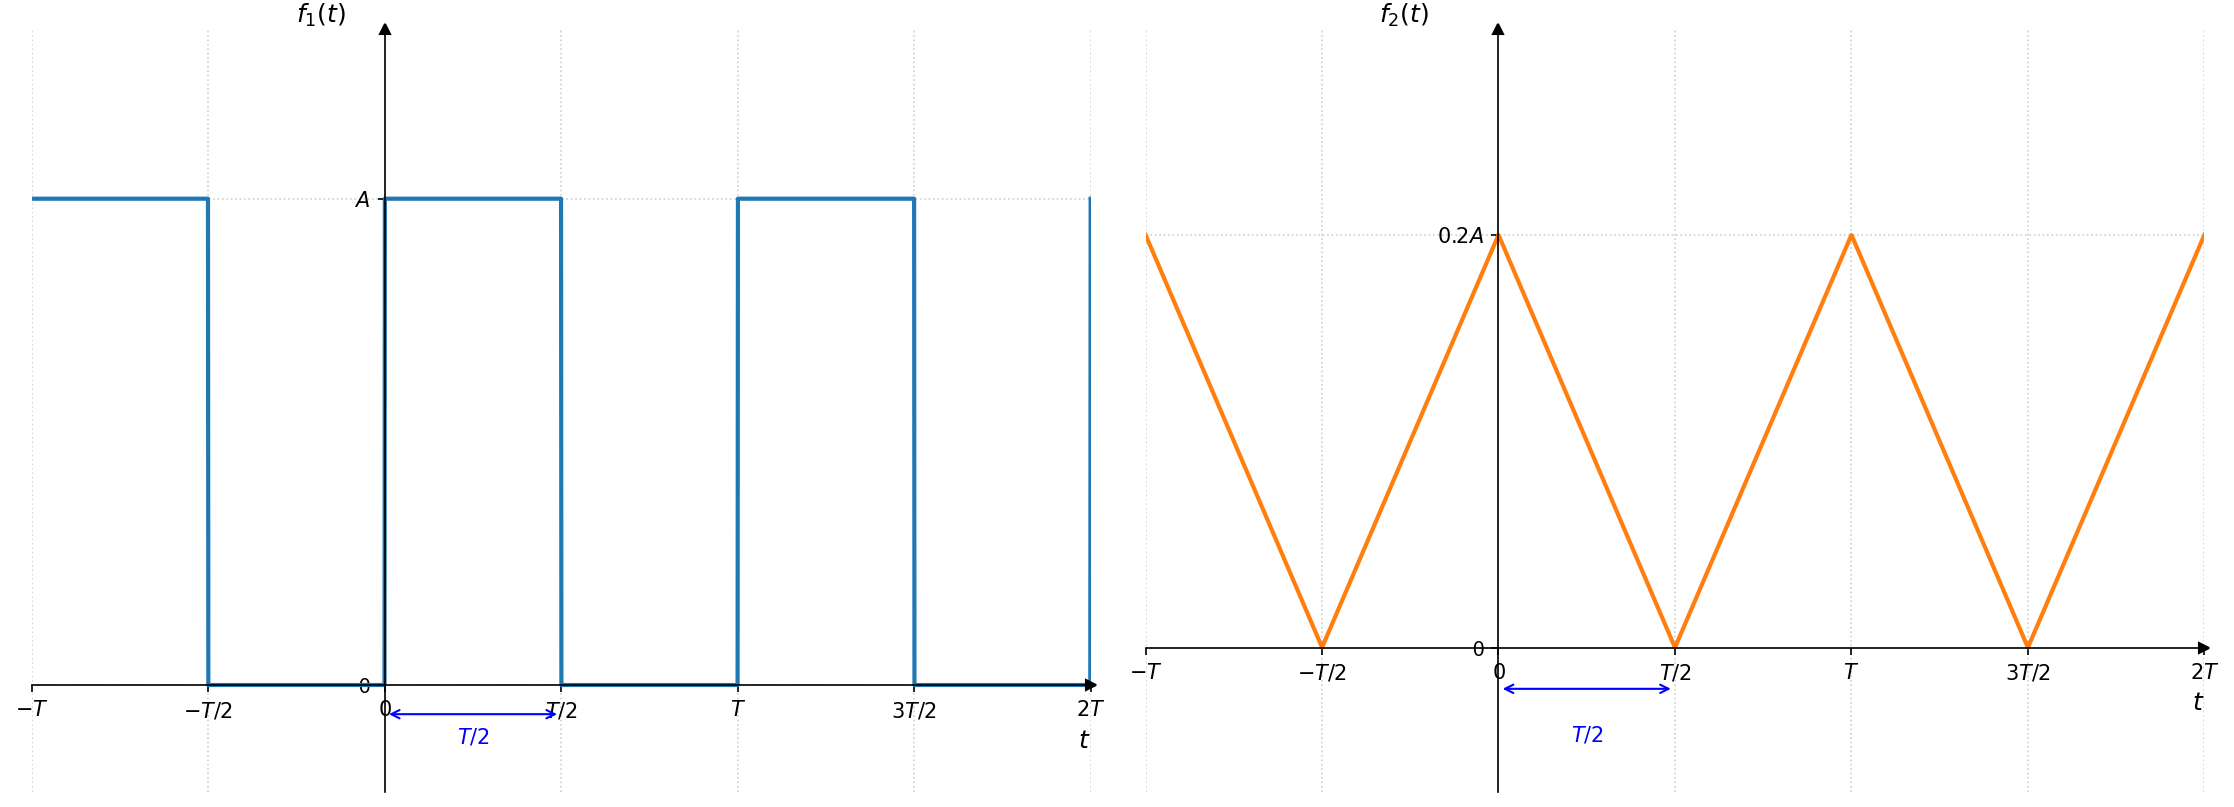
\includegraphics[width=0.5\textwidth]{img/3.6.2.png}
\caption{题3.6分解图}
\end{figure}

对于矩形脉冲 $f_1(t)$，在一个周期内可以取区间$-\dfrac{T}{2}<t<\dfrac{T}{2}$

此时

$$
f_1(t)=
\begin{cases}
0, & -\dfrac{T}{2}<t<0 \\
A, & 0<t<\dfrac{T}{2}
\end{cases}
$$

它的傅里叶级数写成

$$
f_1(t)=\frac{a_0}{2}+\sum_{n=1}^{\infty}\left(a_n\cos n\Omega t+b_n\sin n\Omega t\right)
$$

先算直流分量：

$$
\frac{a_0}{2}
=\frac{1}{T}\int_{-T/2}^{T/2} f_1(t) \mathrm{d}t
=\frac{1}{T}\int_0^{T/2}A \mathrm{d}t
=\frac{A}{2}
$$

再算余弦系数：

$$
a_n=\frac{2}{T}\int_{-T/2}^{T/2}f_1(t)\cos n\Omega t\mathrm{d}t
$$

因为$f_1(t)$ 在$t<0$为$0$，所以只剩

$$
a_n=\frac{2}{T}\int_0^{T/2}A\cos n\Omega t\mathrm{d}t
$$

$$
a_n=
\frac{2A}{T}
\left[\frac{\sin n\Omega t}{n\Omega}\right]_0^{T/2}
$$

代入$\displaystyle n\Omega\frac{T}{2}=n\pi$，则

$$
n\Omega\frac{T}{2}=n\pi
$$

所以

$$
a_n=\frac{2A}{T}\cdot\frac{\sin n\pi}{n\Omega}=0
$$

因此矩形脉冲没有余弦项。

再算正弦系数：

$$
b_n=\frac{2}{T}\int_0^{T/2}A\sin n\Omega t\mathrm{d}t
$$

$$
b_n=
\frac{2A}{T}
\left[-\frac{\cos n\Omega t}{n\Omega}\right]_0^{T/2}
$$

$$
b_n=
\frac{2A}{T}\cdot\frac{1-\cos n\pi}{n\Omega}
$$

由于

$$
\cos n\pi=(-1)^n
$$

所以

$$
b_n=\frac{A}{n\pi}\bigl[1-(-1)^n\bigr]
$$

当 $n$ 为偶数时，$1-(-1)^n=0$，所以

$$
b_n=0
$$

当 $n$ 为奇数时，$1-(-1)^n=2$，所以

$$
b_n=\frac{2A}{n\pi}
$$

因此只保留奇次谐波：

$$
f_1(t)=\frac{A}{2}
+\frac{2A}{\pi}\sum_{k=0}^{\infty}
\frac{1}{2k+1}\sin(2k+1)\Omega t
$$

再看三角脉冲 $f_2(t)$。它的峰值是 $0.2A$，周期为$T$，并且关于 $t=0$ 是偶函数。

在区间$-\frac{T}{2}<t<\frac{T}{2}$内，它可以写成

$$
f_2(t)=\frac{0.4A}{T}|t|
$$

因为在 $t=0$ 时为 $0$，在 $t=\pm T/2$ 时为

$$
\frac{0.4A}{T}\cdot\frac{T}{2}=0.2A
$$

这和图中的三角波一致。

由于$f_2(t)$是偶函数，所以傅里叶级数中只有余弦项，没有正弦项：

$$
b_n=0
$$

先算直流分量。一个周期内三角形面积为

$$
\frac{1}{2}\cdot T\cdot 0.2A=0.1AT
$$

所以平均值为

$$
\frac{a_0}{2}
=\frac{0.1AT}{T}
=0.1A
=\frac{A}{10}
$$

接着算余弦系数：

$$
a_n=\frac{2}{T}\int_{-T/2}^{T/2}f_2(t)\cos n\Omega t\mathrm{d}t
$$

由于 $f_2(t)$ 是偶函数，$\cos n\Omega t$ 也是偶函数，所以

$$
a_n=\frac{4}{T}\int_0^{T/2}
\frac{0.4A}{T}t\cos n\Omega t\,dt
$$

即

$$
a_n=\frac{1.6A}{T^2}\int_0^{T/2}t\cos n\Omega t\,dt
$$

计算积分：

$$
\int t\cos n\Omega t\,dt
=\frac{t\sin n\Omega t}{n\Omega}
+\frac{\cos n\Omega t}{(n\Omega)^2}
$$

所以

$$
\int_0^{T/2}t\cos n\Omega t\,dt
=\left[
\frac{t\sin n\Omega t}{n\Omega}
+\frac{\cos n\Omega t}{(n\Omega)^2}
\right]_0^{T/2}
$$

代入上限：

$$
\sin n\Omega\frac{T}{2}=\sin n\pi=0
$$

$$
\cos n\Omega\frac{T}{2}=\cos n\pi=(-1)^n
$$

因此

$$
\int_0^{T/2}t\cos n\Omega t\,dt
=\frac{(-1)^n-1}{(n\Omega)^2}
$$

于是

$$
a_n=\frac{1.6A}{T^2}\cdot\frac{(-1)^n-1}{(n\Omega)^2}
$$

又因为

$$
\Omega=\frac{2\pi}{T}
$$

所以

$$
(n\Omega)^2=\frac{4n^2\pi^2}{T^2}
$$

代入得

$$
a_n=
\frac{1.6A}{T^2}\cdot\frac{T^2}{4n^2\pi^2}\bigl[(-1)^n-1\bigr]
$$

$$
a_n=\frac{0.4A}{n^2\pi^2}\bigl[(-1)^n-1\bigr]
$$

当 $n$ 为偶数时：

$$
(-1)^n-1=0
$$

所以偶次余弦项为 $0$。

当 $n$ 为奇数时：

$$
(-1)^n-1=-2
$$

所以

$$
a_n=-\frac{0.8A}{n^2\pi^2}
$$

因此三角脉冲的傅里叶级数为

$$
f_2(t)
=\frac{A}{10}
-\frac{0.8A}{\pi^2}\sum_{k=0}^{\infty}
\frac{1}{(2k+1)^2}\cos(2k+1)\Omega t
$$

回到原信号$f(t)=f_1(t)-f_2(t)$

代入两个傅里叶级数：

$$
f_1(t)=
\frac{A}{2}
+\frac{2A}{\pi}\sum_{k=0}^{\infty}
\frac{1}{2k+1}\sin(2k+1)\Omega t
$$

$$
f_2(t)=
\frac{A}{10}
-\frac{0.8A}{\pi^2}\sum_{k=0}^{\infty}
\frac{1}{(2k+1)^2}\cos(2k+1)\Omega t
$$

所以

$$
f(t)=
\left[
\frac{A}{2}
+\frac{2A}{\pi}\sum_{k=0}^{\infty}
\frac{1}{2k+1}\sin(2k+1)\Omega t
\right]
-
\left[
\frac{A}{10}
-\frac{0.8A}{\pi^2}\sum_{k=0}^{\infty}
\frac{1}{(2k+1)^2}\cos(2k+1)\Omega t
\right]
$$

因此最终答案为

$$
f(t)=0.4A
+\frac{2A}{\pi}\sum_{k=0}^{\infty}
\frac{1}{2k+1}\sin(2k+1)\Omega t
+\frac{0.8A}{\pi^2}\sum_{k=0}^{\infty}
\frac{1}{(2k+1)^2}\cos(2k+1)\Omega t
$$
\end{solution}

\subsection{3.12}

\begin{problem}
利用傅里叶变换的频移特性求如图所示信号的傅里叶变换

\begin{figure}[H]
\centering
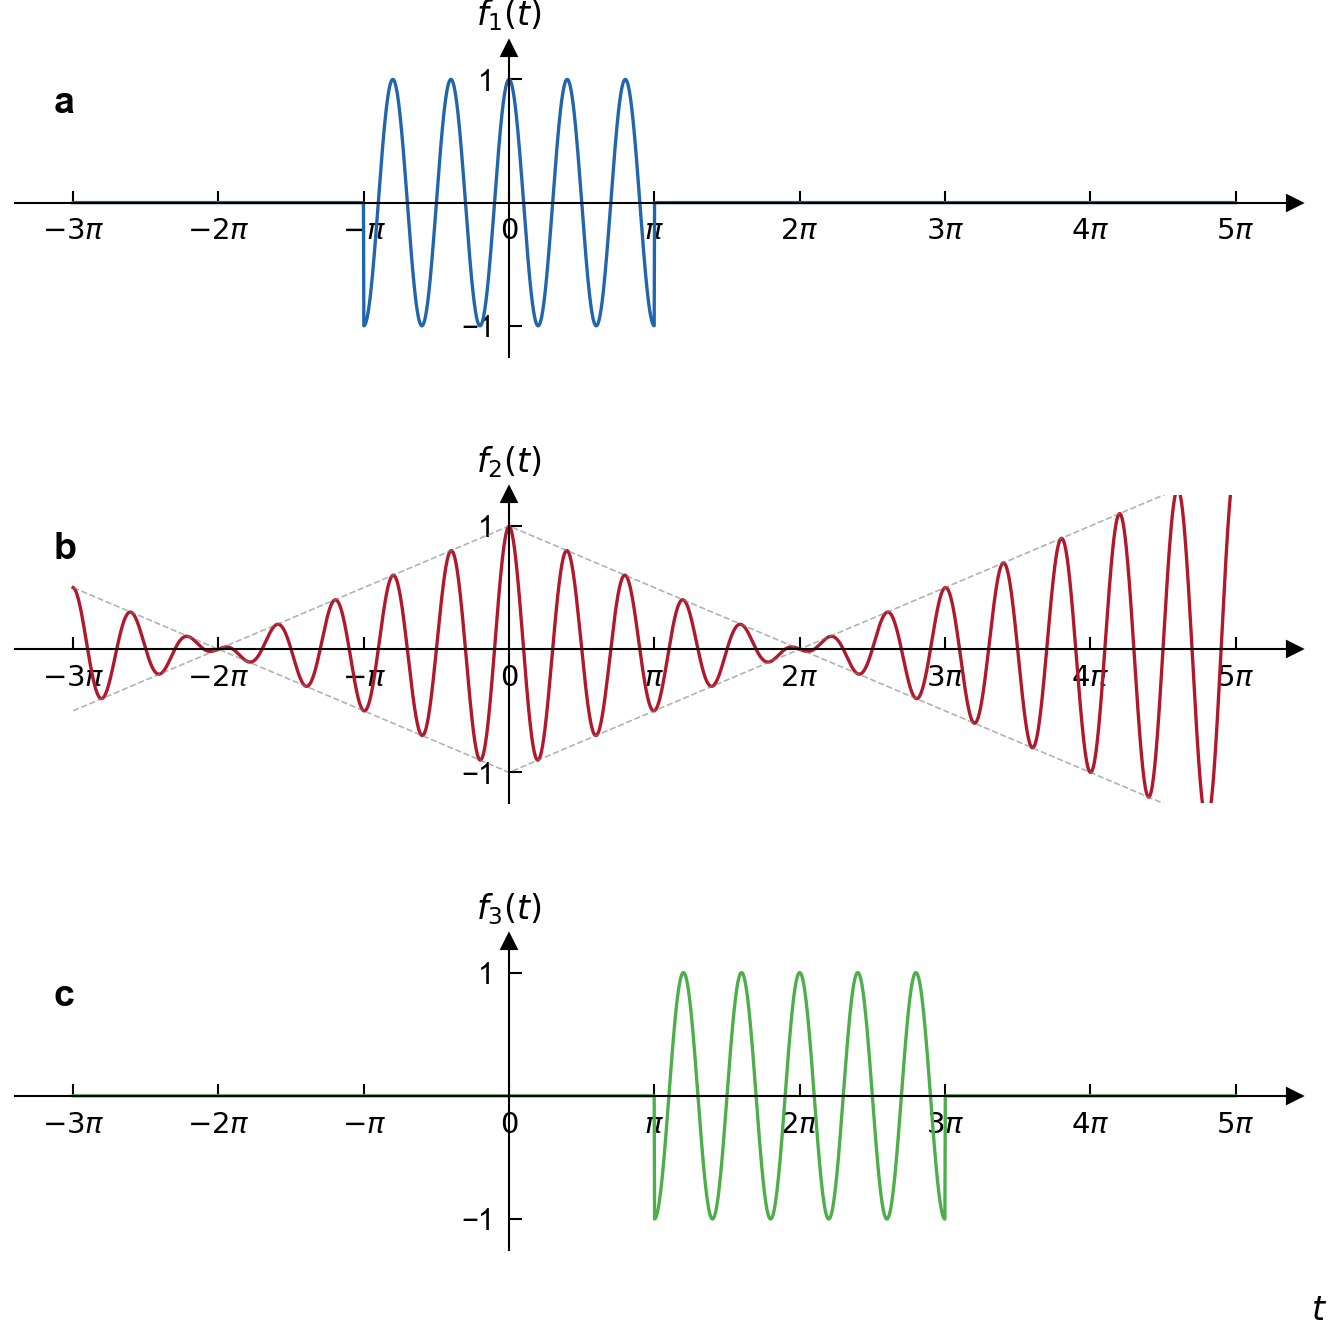
\includegraphics[width=0.5\textwidth]{img/3.12.png}
\caption{题3.12图}
\end{figure}
\end{problem}

\begin{solution}
(a) 由图(a)可知

$$
f_1(t) = \cos 5t \left[\varepsilon(t+\pi) - \varepsilon(t-\pi) \right] = (\cos 5t) \cdot G_{2\pi}(t)
$$

其中$G_{2\pi}(t) = \varepsilon(t+\pi) - \varepsilon(t-\pi)$

因为
$$
G_{2\pi}(t) \longleftrightarrow 2\pi \,\mathrm{Sa}(\pi\omega)
$$

由傅里叶变换的移频性质知
$$
f(t)\cos(\omega_0 t) \longleftrightarrow \frac{1}{2}F[j(\omega+\omega_0)] + \frac{1}{2}F[j(\omega-\omega_0)]
$$

所以

$$
f_1(t) \longleftrightarrow \frac{1}{2} \cdot 2\pi \left\{ \mathrm{Sa}[\pi(\omega+5)] + \mathrm{Sa}[\pi(\omega-5)] \right\}
$$

$$
F_1(j\omega) = \pi \left\{ \mathrm{Sa}[\pi(\omega+5)] + \mathrm{Sa}[\pi(\omega-5)] \right\}
$$

(b) 由图(b)可知

$$
f_2(t) = \cos 5t \cdot \left( 1 - \frac{|t|}{2\pi} \right)
$$

因为 $1 - \dfrac{|t|}{2\pi} \longleftrightarrow \pi \,\mathrm{Sa}^2\left(\dfrac{\pi\omega}{2}\right)$，所以由移频性质得

$$
F_2(j\omega) = \frac{\pi}{2} \left[ \mathrm{Sa}^2 \frac{\pi(\omega+5)}{2} + \mathrm{Sa}^2 \frac{\pi(\omega-5)}{2} \right]
$$

(c) 由图(c)可知，其波形由图(a)右移$2\pi$后得到，所以
$$
f_3(t)=\cos5t \left[\varepsilon(t-\pi)-\varepsilon(t-3\pi)\right]
$$
利用时移特性
$$
\left[\varepsilon(t-\pi)-\varepsilon(t-3\pi)\right] \longleftrightarrow 2\pi\operatorname{Sa}(\pi\omega)\mathrm{e}^{-j2\pi\omega}
$$
所以
$$
F_3(j\omega)=\pi\left\{\operatorname{Sa}\left[\pi(\omega+5)\right]+\operatorname{Sa}\left[\pi(\omega-5)\right]\right\}\mathrm{e}^{-2\pi j\omega}
$$
\end{solution}

\subsection{3.16}

\begin{problem}
试用下列特性求对应信号的傅里叶变换
\begin{enumerate}
    \item 用延时与线性特性；
    \item 用时域微分、积分特性。
\end{enumerate}

\begin{figure}[H]
\centering
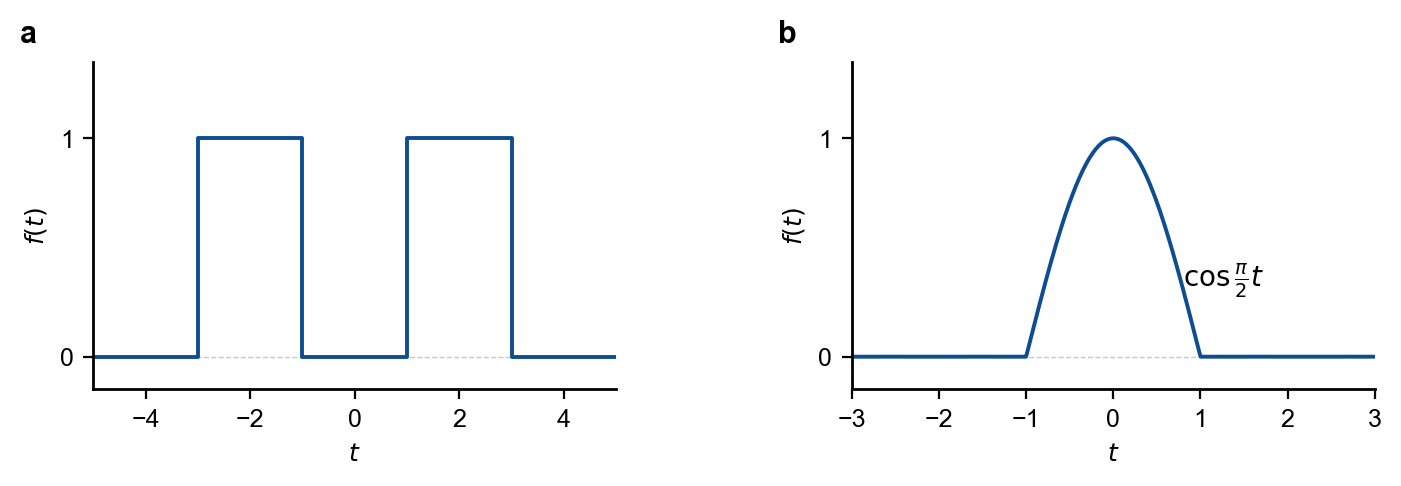
\includegraphics[width=0.5\textwidth]{img/3.16.png}
\caption{题3.16图}
\end{figure}
\end{problem}

\begin{solution}
图(a)对应信号
$$
f(t)=G_{2}(t) \cos \frac{\pi}{2} t
$$

方法一：延时与线性特性
已知变换对：
$$
G_{2}(t) \leftrightarrow 2 \mathrm{Sa}(\omega)
$$

$$
G_{2}(t+2) \leftrightarrow 2 \mathrm{Sa}(\omega)\mathrm{e}^{j2\omega}
$$

$$
G_{2}(t-2) \leftrightarrow 2 \mathrm{Sa}(\omega)\mathrm{e}^{-j2\omega}
$$

所以
$$
\begin{aligned}
F(j \omega) &= 2 \mathrm{Sa}(\omega)\mathrm{e}^{j2\omega} + 2 \mathrm{Sa}(\omega)\mathrm{e}^{-j2\omega} \\
&=4 \mathrm{Sa}(\omega)\cos(2\omega) \\
&= \frac2\omega \left(\sin 3\omega - \sin\omega\right)
\end{aligned}
$$


方法二：时域微分、积分特性

对信号求一阶导数：
$$
\begin{aligned}
f'(t) &= \delta(t+3)-\delta(t+1)+\delta(t-1)-\delta(t-3) \\
&\leftrightarrow e^{j3\omega}-e^{j\omega}+e^{-j\omega}-e^{-j3\omega}=j 4 \sin \omega \cos 2 \omega \\
&= \frac{2}{\omega}(\sin 3 \omega-\sin \omega) \cdot j \omega
\end{aligned}
$$

即
$$
f'(t) \leftrightarrow \frac{2}{\omega}(\sin 3 \omega-\sin \omega) \cdot j \omega
$$

结合时域微分特性，求得原信号频谱：
$$
f(t) \leftrightarrow \frac{2}{\omega}(\sin 3 \omega-\sin \omega)
$$

图(b)对应信号：
$$
f(t)=G_{2}(t) \cos \frac{\pi}{2} t
$$

方法一：延时与线性特性

已知变换对：
$$
G_{2}(t) \leftrightarrow 2 \mathrm{Sa}(\omega)
$$

$$
\cos \frac{\pi}{2} t \leftrightarrow \pi\left[\delta\left(\omega+\frac{\pi}{2}\right)+\delta\left(\omega-\frac{\pi}{2}\right)\right]
$$

根据频域卷积性质计算频谱：
$$
\begin{aligned}
F(j \omega) &= \frac{1}{2 \pi}\left\{2 \mathrm{Sa}(\omega) * \pi\left[\delta\left(\omega+\frac{\pi}{2}\right)+\delta\left(\omega-\frac{\pi}{2}\right)\right]\right\} \\
&= \mathrm{Sa}(\omega) * \delta\left(\omega+\frac{\pi}{2}\right)+\mathrm{Sa}(\omega) * \delta\left(\omega-\frac{\pi}{2}\right) \\
&= \mathrm{Sa}\left(\omega+\frac{\pi}{2}\right)+\mathrm{Sa}\left(\omega-\frac{\pi}{2}\right) \\
&= \frac{4 \pi \cos \omega}{\pi^{2}-4 \omega^{2}}
\end{aligned}
$$

方法二：时域微分、积分特性

将信号改写为：
$$
f(t)=\left(\cos \frac{\pi}{2} t\right) \cdot[\varepsilon(t+1)-\varepsilon(t-1)]
$$

对信号求一阶导数：
$$
\begin{aligned}
f'(t) &= \left(-\frac{\pi}{2} \sin \frac{\pi}{2} t\right) \cdot[\varepsilon(t+1)-\varepsilon(t-1)]+\cos \frac{\pi}{2} t[\delta(t+1)-\delta(t-1)] \\
&= \left(-\frac{\pi}{2} \sin \frac{\pi}{2} t\right) \cdot[\varepsilon(t+1)-\varepsilon(t-1)]
\end{aligned}
$$

对信号求二阶导数：
$$
\begin{aligned}
f''(t) &= \left[-\frac{\pi^{2}}{4} \cos \frac{\pi}{2} t\right] \cdot[\varepsilon(t+1)-\varepsilon(t-1)] - \frac{\pi}{2} \sin \frac{\pi}{2} t \cdot [\delta(t+1)-\delta(t-1)] \\
&= -\frac{\pi^{2}}{4} f(t)+\frac{\pi}{2} \delta(t+1)+\frac{\pi}{2} \delta(t-1)
\end{aligned}
$$

对等式两侧取傅里叶变换：
$$
\begin{aligned}
f''(t) &\leftrightarrow -\frac{\pi^{2}}{4} F(j \omega)+\frac{\pi}{2} e^{j\omega}+\frac{\pi}{2} e^{-j \omega} \\
&= -\frac{\pi^{2}}{4} F(j \omega)+\pi \cos \omega = (j \omega)^{2} F(j \omega)
\end{aligned}
$$

整理求解频谱：
$$
F(j \omega)=\frac{\pi \cos \omega}{(j \omega)^{2}+\frac{\pi^{2}}{4}}=\frac{4 \pi \cos \omega}{\pi^{2}-4 \omega^{2}}
$$

\begin{figure}[H]
\centering
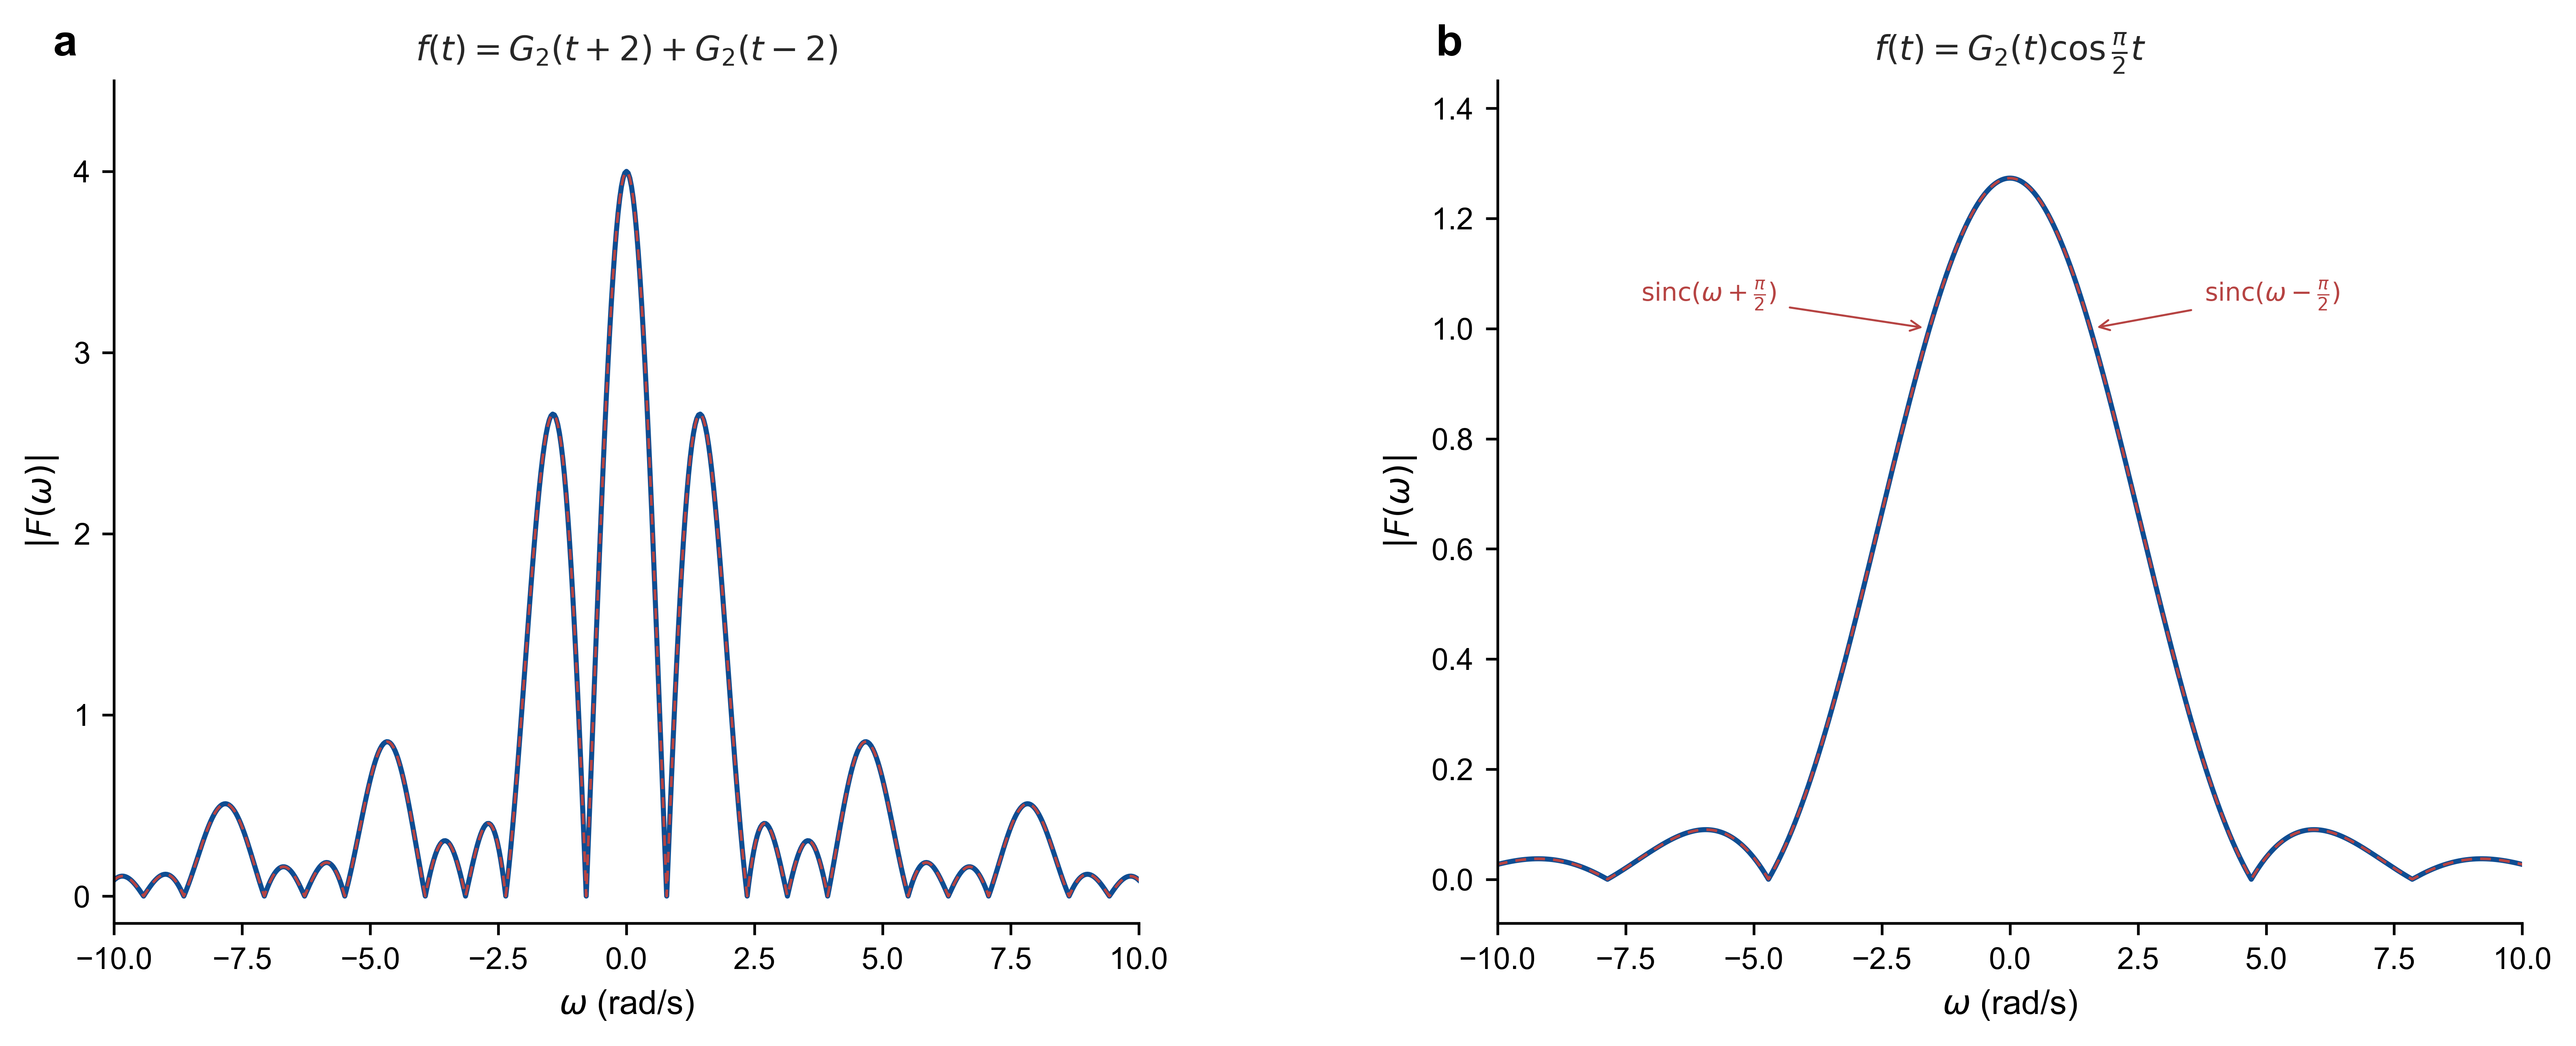
\includegraphics[width=0.5\textwidth]{img/3.16.2.png}
\caption{题3.16图(b)解法}
\end{figure}
\end{solution}

\subsection{3.20}

\begin{problem}
由冲激函数的傅里叶变换求如图所示波形信号的傅里叶变换

\begin{figure}[H]
\centering
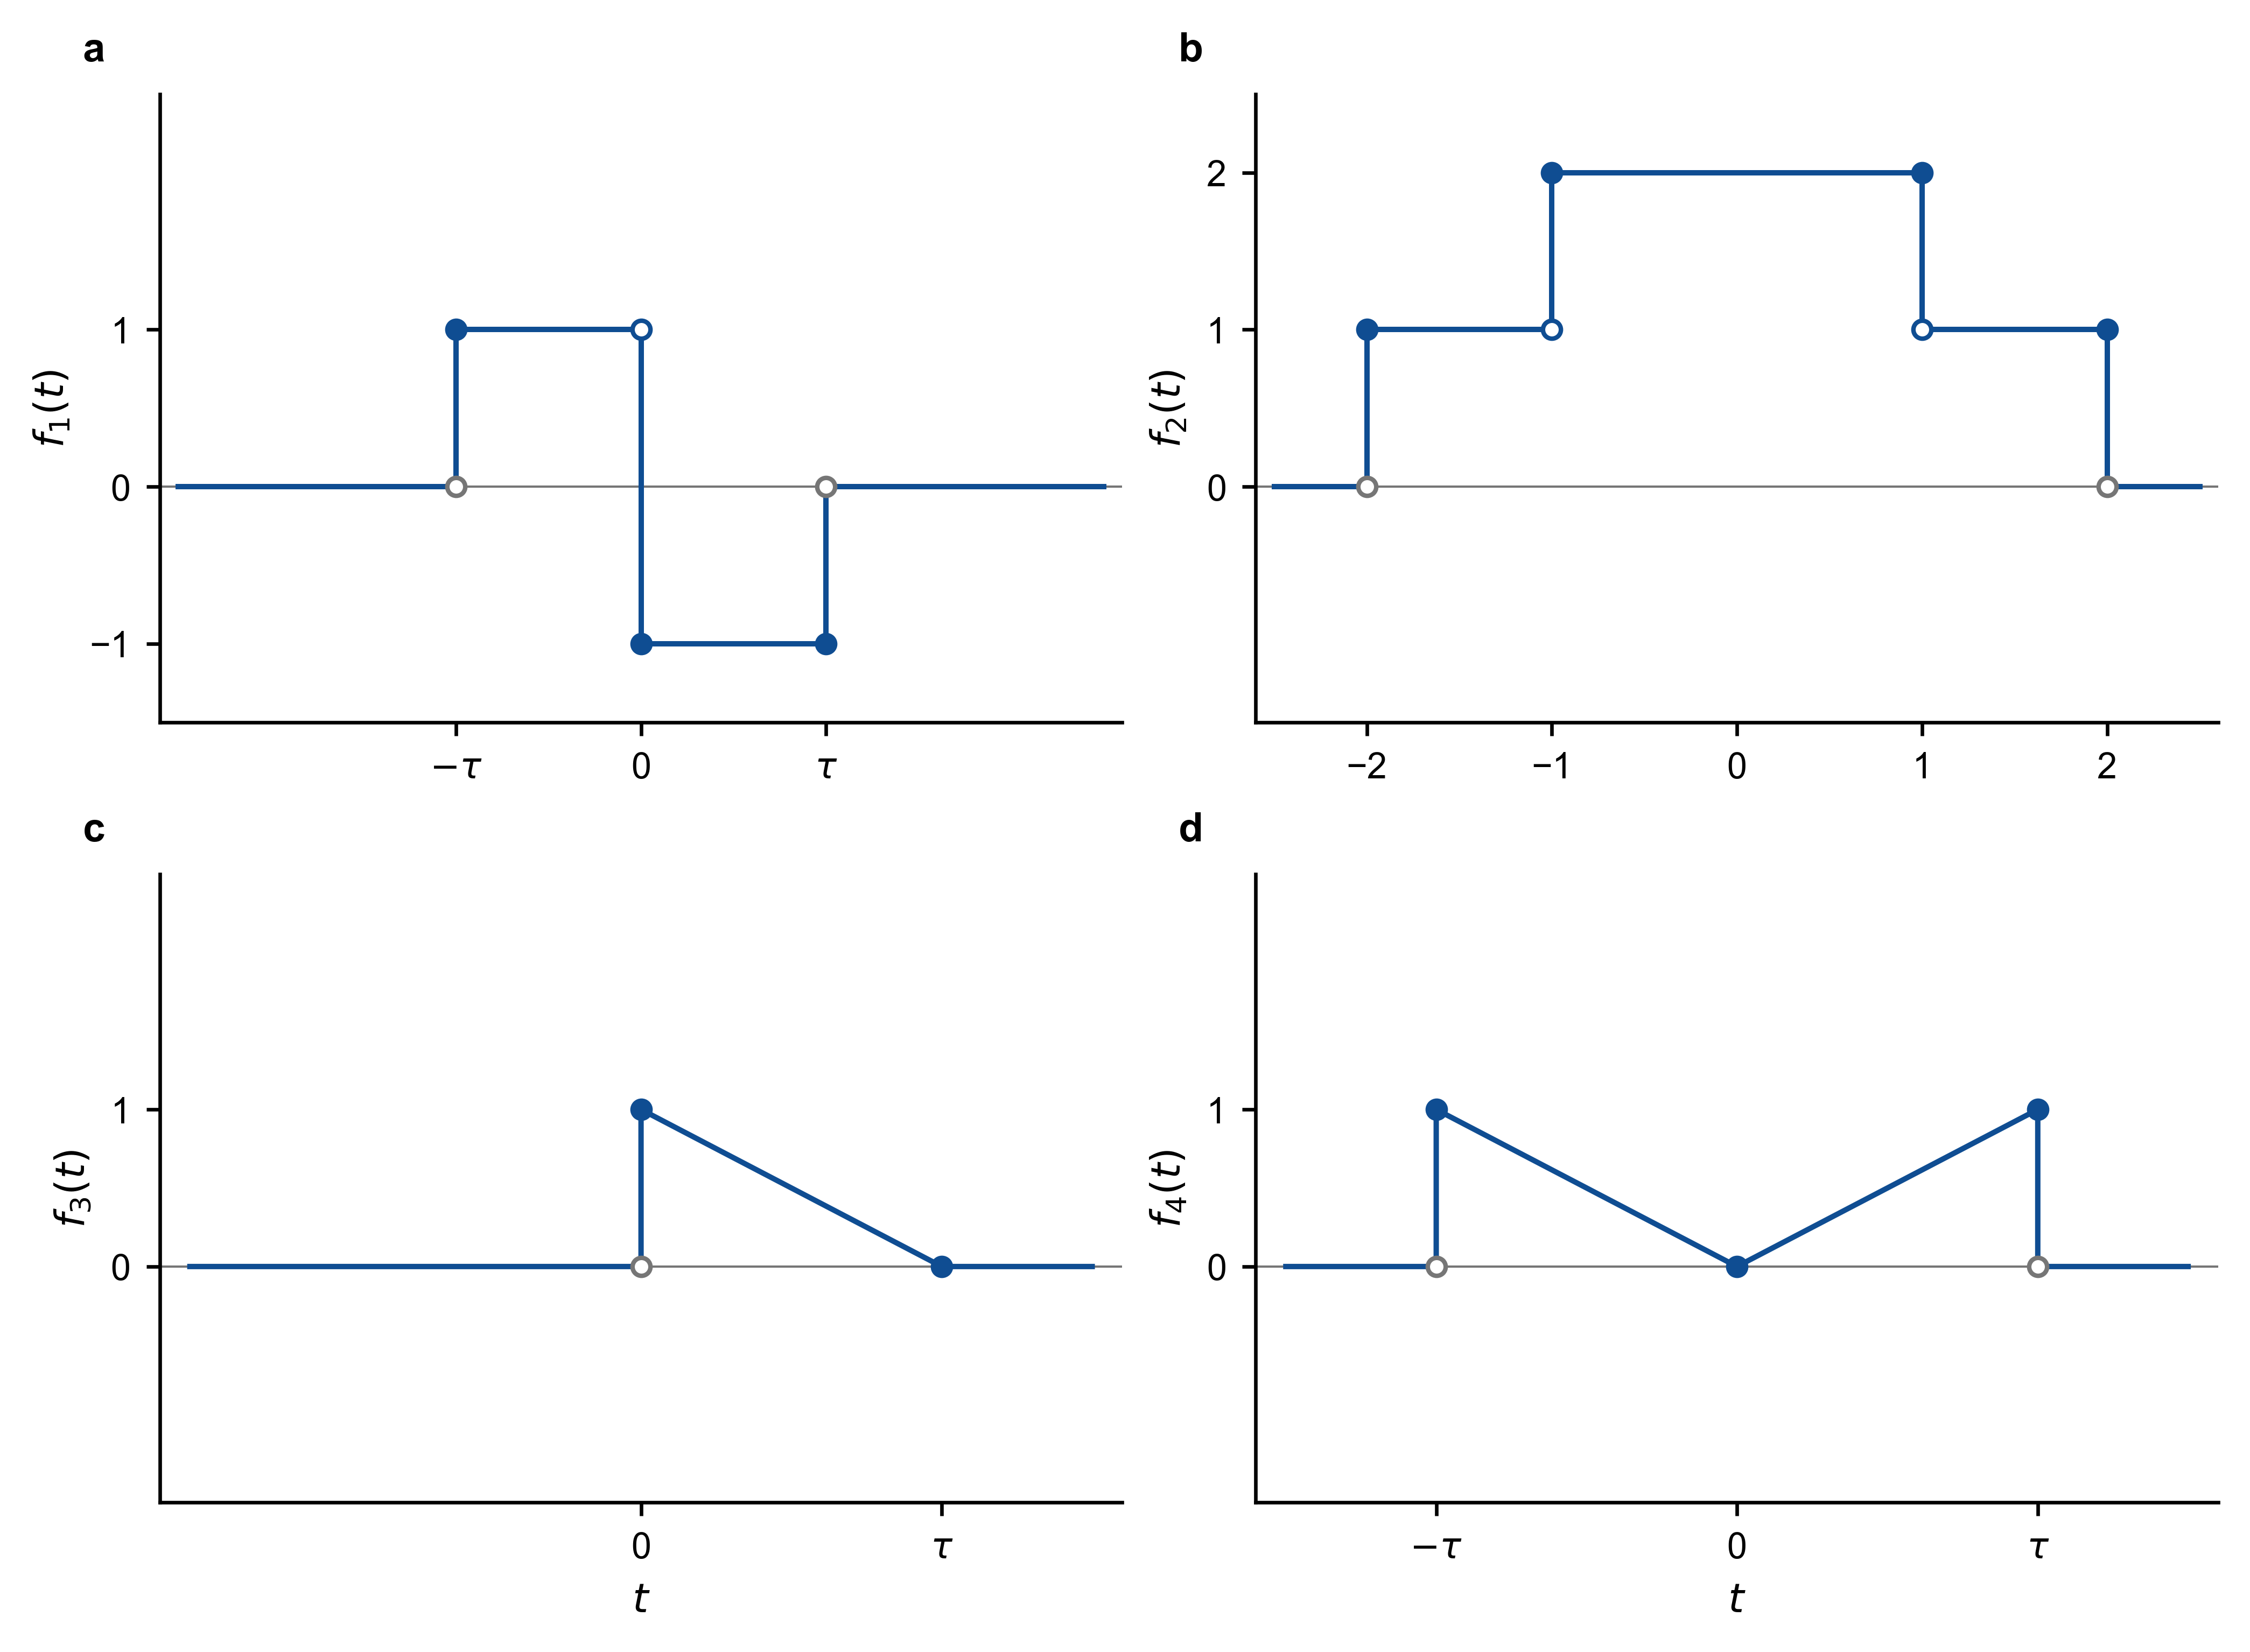
\includegraphics[width=0.5\textwidth]{img/3.20.png}
\caption{题3.20图}
\end{figure}

对任意信号$f(t)$，由微积分关系可得
$$
f(t)=\int_{-\infty}^t f^\prime(\xi)\mathrm{d}\xi
$$
根据卷积定义，时域积分运算等价于信号与单位阶跃函数做卷积：
$$
\int_{-\infty}^{t} f_1'(\xi) \,\mathrm{d}\xi
= f_1'(t) * \varepsilon(t)
$$
时域卷积定理：若
$$
g(t) \leftrightarrow G(j\omega),\quad h(t) \leftrightarrow H(j\omega)
$$
则时域卷积对应频域相乘：
$$
g(t) * h(t) \leftrightarrow G(j\omega) \cdot H(j\omega)
$$
单位阶跃函数的傅里叶变换公式：
$$
\varepsilon(t) \leftrightarrow \frac{1}{j\omega} + \pi \delta(\omega)
$$
代入得
$$
f(t) \leftrightarrow \left[\frac{1}{j\omega} + \pi \delta(\omega)\right] \cdot \mathscr{F}\{f^\prime(t)\}
$$
\end{problem}

\begin{solution}
(1)
$$
f_{1}(t)=[\varepsilon(t+\tau)-\varepsilon(t)]-[\varepsilon(t)-\varepsilon(t-\tau)]
$$

对信号求一阶导数并进行傅里叶变换：

$$
\begin{aligned}
f_{1}'(t) &= \delta(t+\tau)-\delta(t)-\delta(t)-\delta(t-\tau) \\
&\leftrightarrow e^{j \omega \tau}-2+e^{-j \omega \tau} \\
&= 2 \cos (\omega \tau)-2
\end{aligned}
$$

结合时域积分特性求解原信号频谱：

$$
f_{1}(t) \leftrightarrow\left[\frac{1}{j \omega}+\pi \delta(\omega)\right] \cdot[2 \cos (\omega \tau)-2]=\frac{2}{j \omega}[\cos (\omega \tau)-1]=j \frac{4}{\omega} \sin ^{2}\left(\frac{\omega \tau}{2}\right)
$$

(2)

$$
f_{2}(t)=\varepsilon(t+2)+\varepsilon(t+1)-\varepsilon(t-1)-\varepsilon(t-2)
$$

对信号求一阶导数并进行傅里叶变换：

$$
\begin{aligned}
f_{2}'(t) &= \delta(t+2)+\delta(t+1)-\delta(t-1)-\delta(t-2) \\
&\leftrightarrow e^{j 2 \omega}+e^{j \omega}-e^{-j \omega}-e^{-j 2 \omega} \\
&= 2 j(\sin \omega+\sin 2 \omega)
\end{aligned}
$$

结合时域积分特性求解原信号频谱：

$$
f_{2}(t) \leftrightarrow\left[\pi \delta(\omega)+\frac{1}{j \omega}\right] \cdot[2 j(\sin \omega+\sin 2 \omega)]=\frac{2}{\omega}(\sin \omega+\sin 2 \omega)
$$

(3)

$$
f_{3}(t)=-\frac{1}{\tau}(t-\tau)[\varepsilon(t)-\varepsilon(t-\tau)]
$$

对信号求一阶导数：

$$
\begin{aligned}
f_{3}'(t) &= -\frac{1}{\tau}[\varepsilon(t)-\varepsilon(t-\tau)]-\frac{1}{\tau}(t-\tau)[\delta(t)-\delta(t-\tau)] \\
&= -\frac{1}{\tau}[\varepsilon(t)-\varepsilon(t-\tau)]+\delta(t)
\end{aligned}
$$

对一阶导数求二阶导数，并做傅里叶变换：

$$
\begin{aligned}
f_{3}''(t) &= -\frac{1}{\tau}[\delta(t)-\delta(t-\tau)]+\delta'(t) \\
&\leftrightarrow -\frac{1}{\tau}\left(1-e^{-j \omega \tau}\right)+j \omega
\end{aligned}
$$

结合时域微分特性求解原信号频谱：

$$
\begin{aligned}
f_{3}(t) &\leftrightarrow \frac{1}{(j \omega)^{2}}\left[-\frac{1}{\tau}\left(1-e^{-j \omega \tau}\right)+j \omega\right] \\
&= \frac{1}{(j \omega)^{2}}\left[j \omega-\frac{1}{\tau}\left(1-e^{-j \omega \tau}\right)\right] \\
&= \frac{1}{j \omega}+\frac{1}{\tau \omega^{2}}\left(1-e^{-j \omega \tau}\right)
\end{aligned}
$$

(4)

信号组合关系：

$$
f_{4}(t)=f_{3}(t+\tau)+f_{3}(-t+\tau)
$$

结合傅里叶变换延时、反褶特性推导频谱：

$$
\begin{aligned}
f_{4}(t) &\leftrightarrow F_{3}(\omega) e^{j \omega \tau}+F_{3}(-\omega) e^{-j \omega \tau} \\
&= \left[\frac{1}{j \omega}+\frac{1}{\tau \omega^{2}}\left(1-e^{-j \omega \tau}\right)\right] e^{j \omega \tau}+\left[\frac{1}{-j \omega}+\frac{1}{\tau \omega^{2}}\left(1-e^{j \omega \tau}\right)\right] e^{-j \omega \tau} \\
&= 2 \tau \mathrm{Sa}(\omega \tau)-\tau \mathrm{Sa}^{2}\left(\frac{\omega \tau}{2}\right)
\end{aligned}
$$
\end{solution}

\section{LTI系统的频域分析法}

\subsection{LTI系统时域和频域分析法特点}

时域分析法

\begin{itemize}
    \item 以时间为变量。
    
    求解时域中的线性常系数微分方程。
    
    信号分解为冲激函数，利用冲激响应和卷积积分求得系统的零状态响应。
    
    \item 频域分析法
    
    以频率为变量。
    
    求解频域中的代数方程。
    
    信号分解为正弦函数或指数函数，利用Fourier变换将时域问题转换到频域以简化运算。
    
    缺点：增加两次积分运算
\end{itemize}

共同处：利用线性系统的叠加性和齐次性

\subsection{系统函数的定义}

输入激励
$$
e(t) \leftrightarrow E(j\omega)
$$
零状态响应
$$
r(t) \leftrightarrow R(j\omega)
$$

$$
r(t)=e(t) * h(t) \leftrightarrow R(j\omega)=E(j\omega)H(j\omega)
$$

系统函数或频率响应函数：联系频域中零状态响应与输入激励的函数。
$$
H(j\omega)=\dfrac{R(j\omega)}{E(j\omega)}
$$

$$
h(t) \leftrightarrow H(j\omega)
$$

系统函数和单位冲激响应为Fourier变换对

\subsection{系统函数的求解}

对微分方程两边求Fourier变换
时域微分方程：
$$
\frac{\mathrm{d}^n r}{\mathrm{d}t^n} + a_{n-1}\frac{\mathrm{d}^{n-1} r}{\mathrm{d}t^{n-1}} + \dots + a_1\frac{\mathrm{d} r}{\mathrm{d}t} + a_0 r
= b_m\frac{\mathrm{d}^m e}{\mathrm{d}t^m} + b_{m-1}\frac{\mathrm{d}^{m-1} e}{\mathrm{d}t^{m-1}} + \dots + b_1\frac{\mathrm{d} e}{\mathrm{d}t} + b_0 e
$$

Fourier变换微分性质：
$$
f(t) \leftrightarrow F(j\omega)
$$

$$
\frac{\mathrm{d}f(t)}{\mathrm{d}t} \leftrightarrow j\omega F(j\omega)
$$



对方程作Fourier变换：
$$
\left\{ (j\omega)^n + a_{n-1}(j\omega)^{n-1} + \dots + a_1(j\omega) + a_0 \right\} R(j\omega)
= \left\{ b_m(j\omega)^m + b_{m-1}(j\omega)^{m-1} + \dots + b_1(j\omega) + b_0 \right\} E(j\omega)
$$

定义系统函数：
$$
H(j\omega) = \frac{R(j\omega)}{E(j\omega)}
= \frac{b_m(j\omega)^m + b_{m-1}(j\omega)^{m-1} + \dots + b_1(j\omega) + b_0}{(j\omega)^n + a_{n-1}(j\omega)^{n-1} + \dots + a_1(j\omega) + a_0}
$$

\subsection{频域分析法步骤}

\begin{enumerate}
    \item 时域→频域，得到频域的输入激励信号。
    $$
    e(t) \to E(j\omega)
    $$
    
    \item 根据系统方程，找出系统函数$H(j\omega)$。可以得到单位冲激响应
    $$
    H(j\omega) \leftrightarrow h(t)
    $$
    
    \item 在频域中求零状态响应。
    $$
    R(j\omega) = E(j\omega)H(j\omega)
    $$
    
    \item 频域→时域，得到时域的输出信号。
    $$
    R(j\omega) \to r(t)
    $$
\end{enumerate}

时域到频域 → 频域求解代数方程 → 频域到时域

\subsection{无失真传输}

\subsubsection{信号失真的原因}

\begin{itemize}
    \item 系统对组成信号的各个频率分量的幅度衰减程度不同，造成信号各频率分量的相对比例关系发生变化，称为幅度失真。
    \item 系统对组成信号的各个频率分量的相移不与频率成正比，造成信号各频率分量在时间轴上的相对位置关系发生变化，称为相位失真。
    \item 幅度失真和相位失真都没有产生新的频率分量，属于线性失真。
\end{itemize}

\subsubsection{无失真传输}

无失真传输指信号经过传输系统之后，只有幅度大小和出现的时间的不同，信号的形状完全不变。

无失真传输的理想条件：
$$
H(j\omega)=|H(j\omega)|\mathrm{e}^{j\phi(\omega)}=K\mathrm{e}^{-j\omega t_0}
$$

$$
h(t)=K\delta(t-t_0)
$$

相位变化与频率变化成比例

\section{频域分析法例题}

\subsection{例题1}

\begin{problem}
已知系统微分方程和输入激励信号，求响应。
$$
\frac{\mathrm{d}}{\mathrm{d}t}r(t)+2r(t)=e(t) \quad e(t)=e^{-t}\varepsilon(t)
$$
\end{problem}

\begin{solution}
$$
e(t) \leftrightarrow E(j\omega)=\frac{1}{j\omega+1}
$$

由
$$
\mathscr{F}\left[\frac{\mathrm{d}}{\mathrm{d}t}r(t)\right]=j\omega\cdot R(j\omega)
$$
于是
$$
(j\omega+2)R(j\omega)=E(j\omega)
$$

$$
H(j\omega)=\frac{R(j\omega)}{E(j\omega)}=\frac{1}{j\omega+2}
$$

所以
$$
R(j\omega)=H(j\omega)\cdot E(j\omega)=\frac{1}{j\omega+2} \cdot \frac{1}{j\omega+1} = \frac{1}{j\omega+1} - \frac{1}{j\omega+2}
$$

时域的零状态响应：

$$
r(t)=\left[e^{-t}-e^{-2t}\right]\varepsilon(t)
$$
\end{solution}

\subsection{例题2}

\begin{problem}
电路如图所示，求单位冲激响应$u_C(t)$。

\begin{figure}[H]
\centering
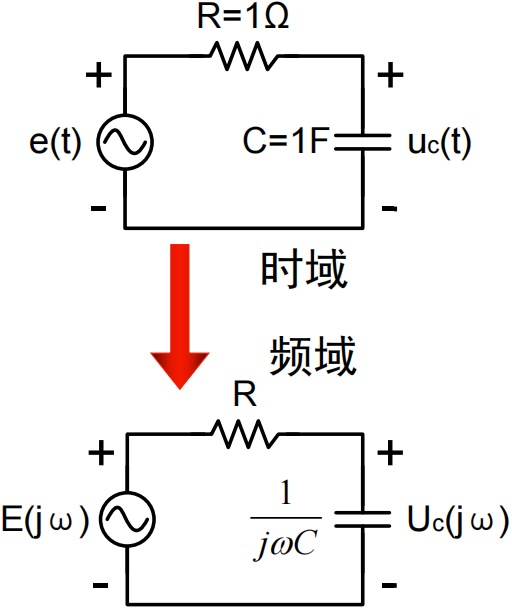
\includegraphics[width=0.5\textwidth]{img/例题4.2.jpg}
\caption{例题2电路图}
\end{figure}
\end{problem}

\begin{solution}
根据频域电路欧姆定律，电容电压的频域表达式：
$$
U_C(j\omega) = I\cdot Z_C = I\frac{1}{j\omega C}
$$
根据KVL
$$
E(j\omega)=U_C(j\omega)+U_R(j\omega)=I\left(R+\frac{1}{j\omega C}\right)
$$
于是
$$
H(j\omega)=\frac{U_C(j\omega)}{E(j\omega)}=\frac{\dfrac{1}{j\omega C}}{\dfrac{1}{j\omega C}+R}
$$
带入数值
$$
H(j\omega)=\frac{1}{j\omega + 1} \leftrightarrow h(t)=e^{-t}\varepsilon(t)
$$
\end{solution}

\subsection{例题3}

\begin{problem}
已知线性系统频响特性和输入激励，求解系统零状态响应。

输入激励信号：
$$
e(t)=2+4 \cos t+4 \cos 2 t
$$

\begin{figure}[H]
\centering
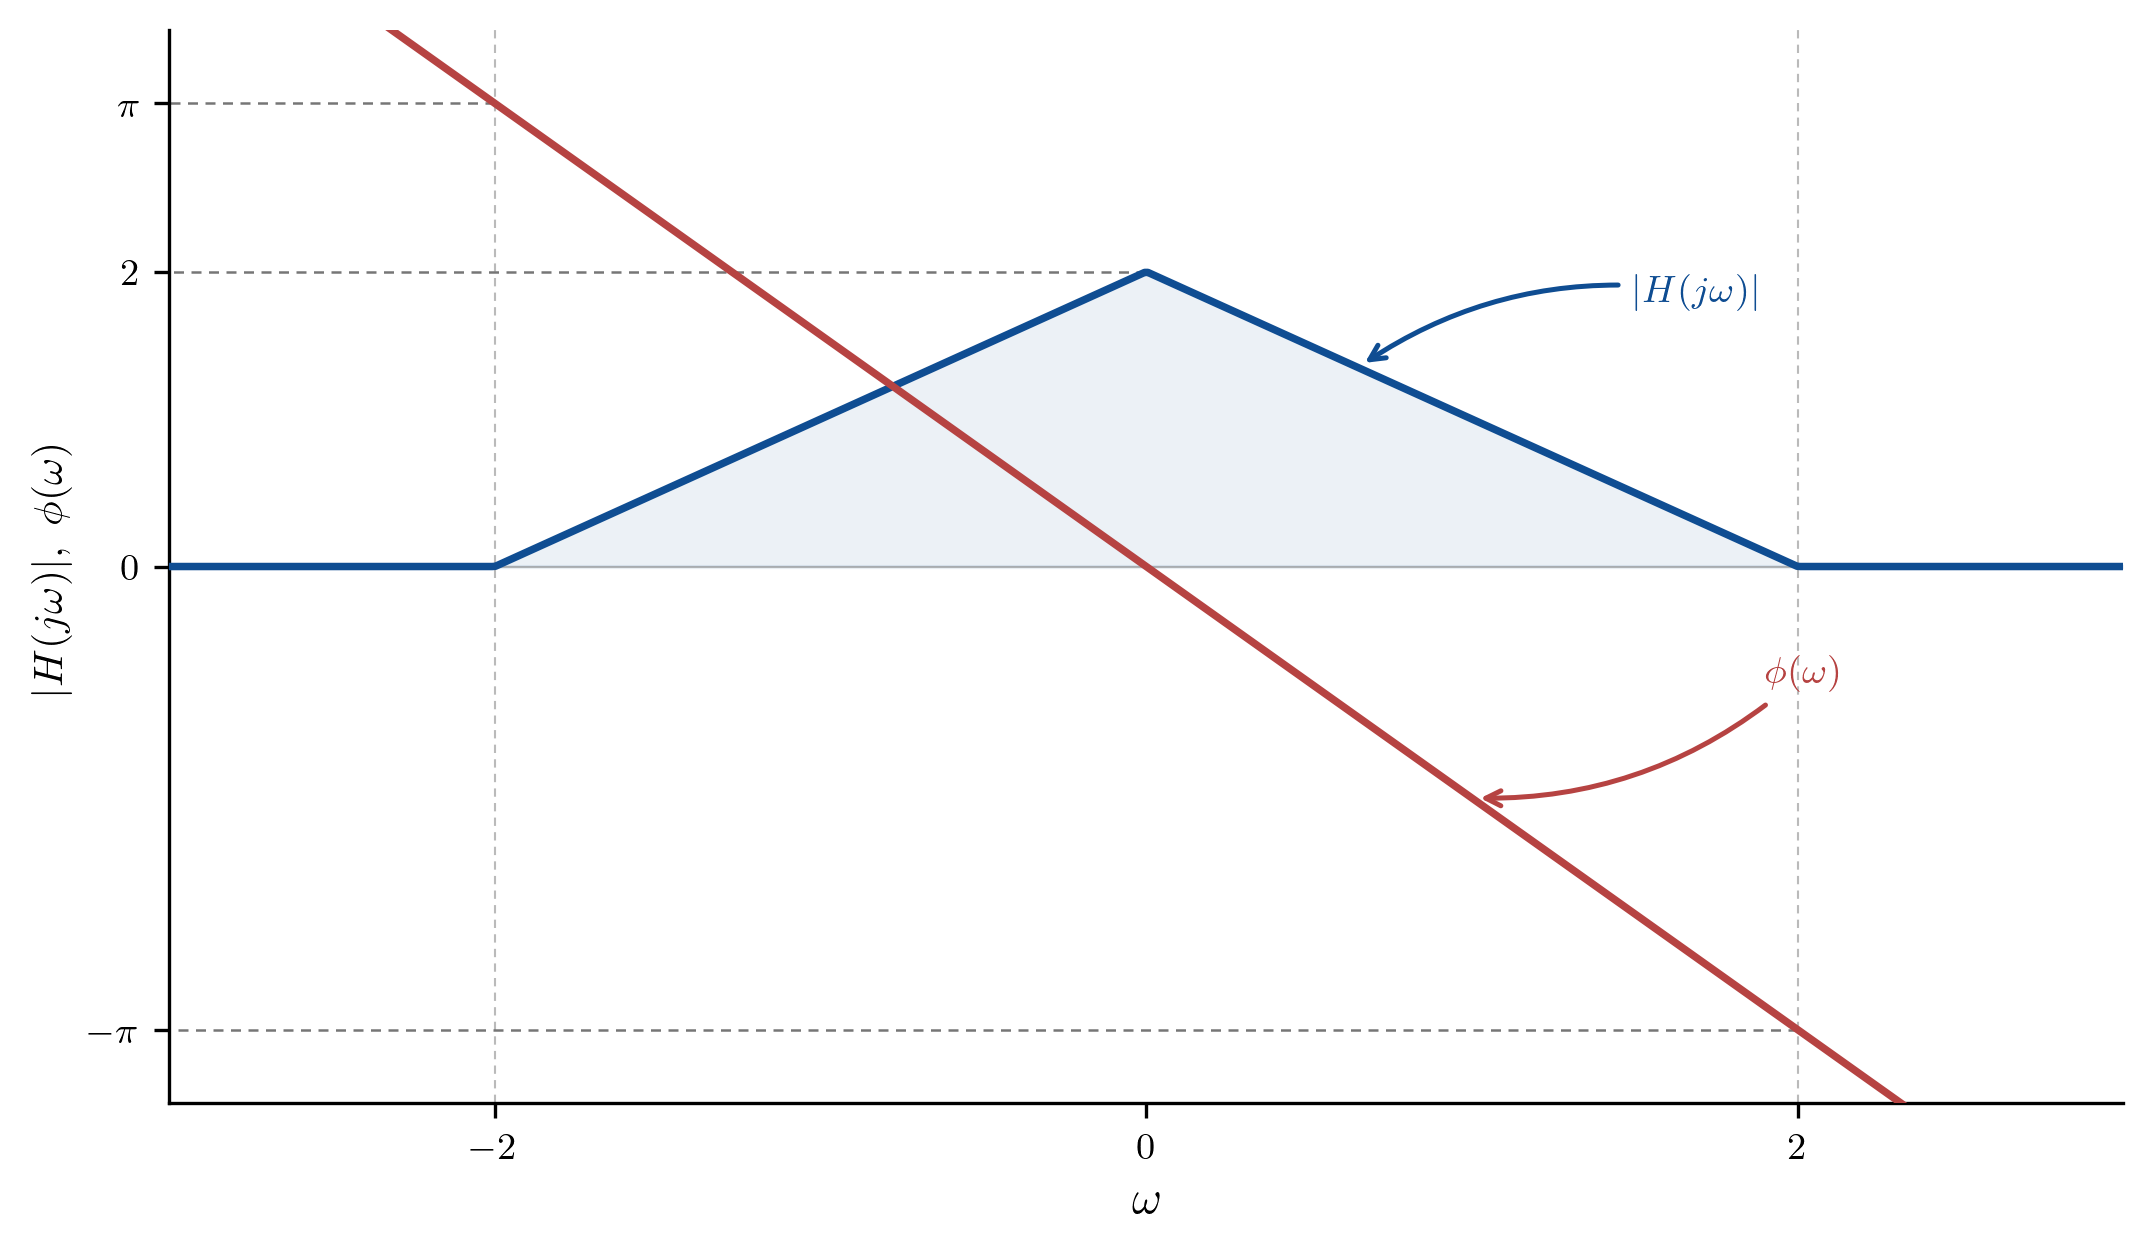
\includegraphics[width=0.5\textwidth]{img/例题4.3.png}
\caption{例题3频响特性}
\end{figure}
\end{problem}

\begin{solution}
对输入信号做时域到频域变换，求解$E(j\omega)$

$$
\begin{aligned}
E(j \omega) =&4 \pi \delta(\omega)+4 \pi[\delta(\omega+1)+\delta(\omega-1)] \\
& +4 \pi[\delta(\omega+2)+\delta(\omega-2)]
\end{aligned}
$$

系统频率响应$H(j\omega)$

$$
H(j \omega)=
\begin{cases}
(2-|\omega|) e^{-j \frac{\pi}{2} \omega} & |\omega|<2 \\
0 & |\omega| \geq 2
\end{cases}
$$

冲激筛选：对任意连续函数$f(\omega)$，有
$$
f(\omega)\cdot \delta(\omega-\omega_0) = f(\omega_0)\cdot \delta(\omega-\omega_0)
$$

频域求解输出信号频谱$R(j\omega)$：

由LTI系统频域关系 $R(j\omega) = E(j\omega)H(j\omega)$，代入计算：
$$
\begin{aligned}
R(j \omega) & =E(j \omega) H(j \omega) \\
& =8 \pi \delta(\omega)+4 \pi \delta(\omega+1) e^{j \frac{\pi}{2}}+4 \pi \delta(\omega-1) e^{-j \frac{\pi}{2}}
\end{aligned}
$$

频域到时域逆变换：
$$
r(t)=4+4 \cos \left(t-\frac{\pi}{2}\right)=4+4 \sin t
$$
\end{solution}

\section{取样信号与取样定理}

\subsection{离散时间信号——序列}

离散时间信号可以通过对连续时间信号进行取样得到，通常采用均匀时间间隔。若时间间隔为$T$，离散时间信号可以用$x(nT)$，或$x(n)$来表示，$n$为整数。

\begin{figure}[H]
\centering
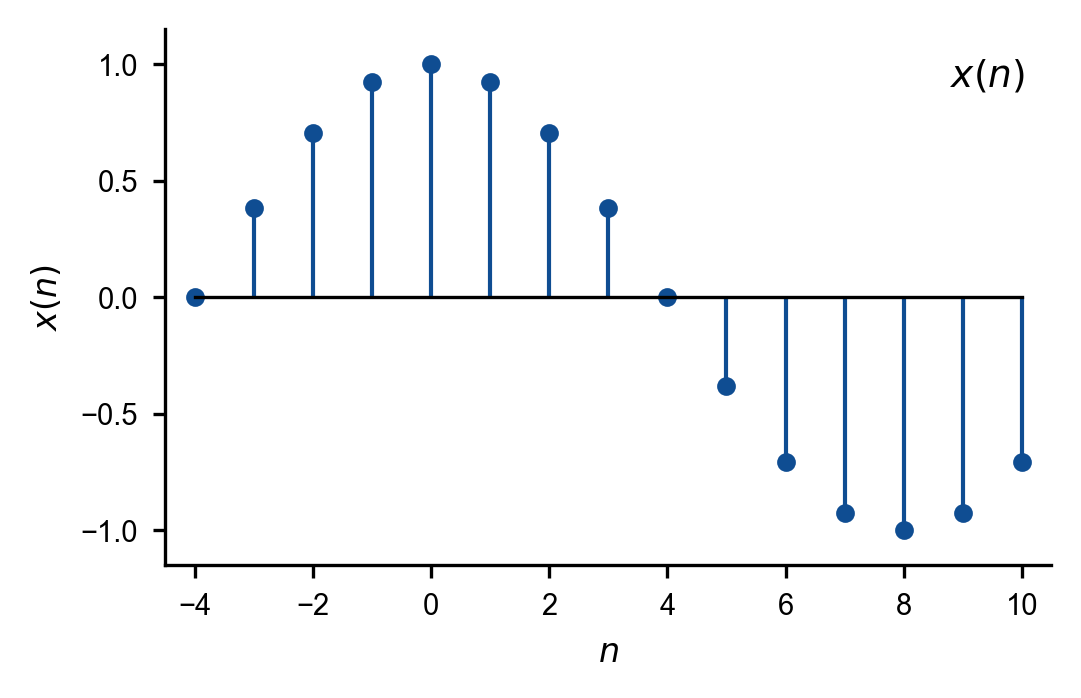
\includegraphics[width=0.5\textwidth]{img/笔记7.1.png}
\caption{离散时间信号}
\end{figure}

\subsection{典型序列}

单位函数序列
$$
\delta(k)=\begin{cases}1, &k=0 \\ 0, &k\neq 0\end{cases}
$$

$$
\delta(k-n)=\begin{cases}1, &k=n \\ 0, &k\neq n\end{cases}
$$

\begin{figure}[H]
\centering
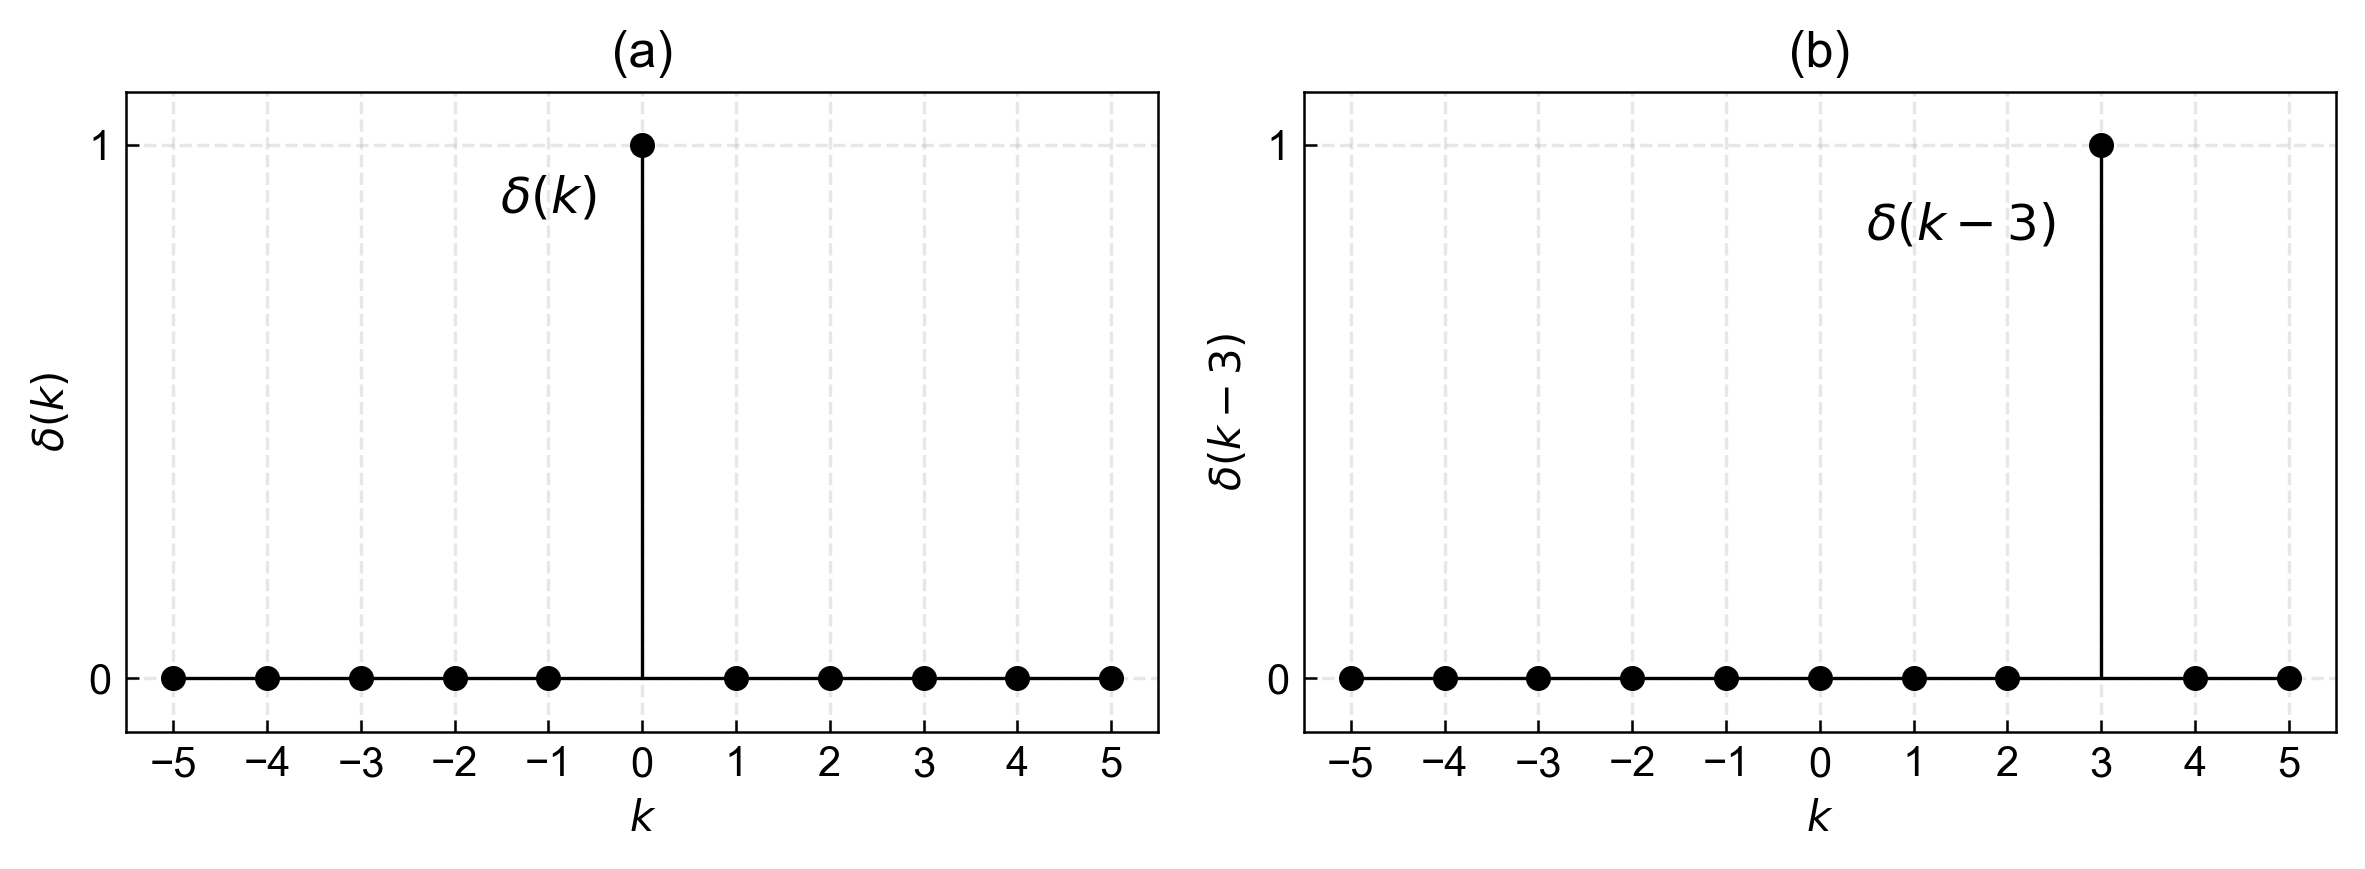
\includegraphics[width=0.5\textwidth]{img/笔记7.2.png}
\caption{单位函数序列}
\end{figure}

单位阶跃序列
$$
\varepsilon(k)=
\begin{cases}
1 & k \geq 0 \\
0 & k<0
\end{cases}
$$

$$
\varepsilon(k-n)=
\begin{cases}
1 & k \geq n \\
0 & k<n
\end{cases}
$$

单边指数序列
$$
e^{-k} \varepsilon(k)
$$

\begin{figure}[H]
\centering
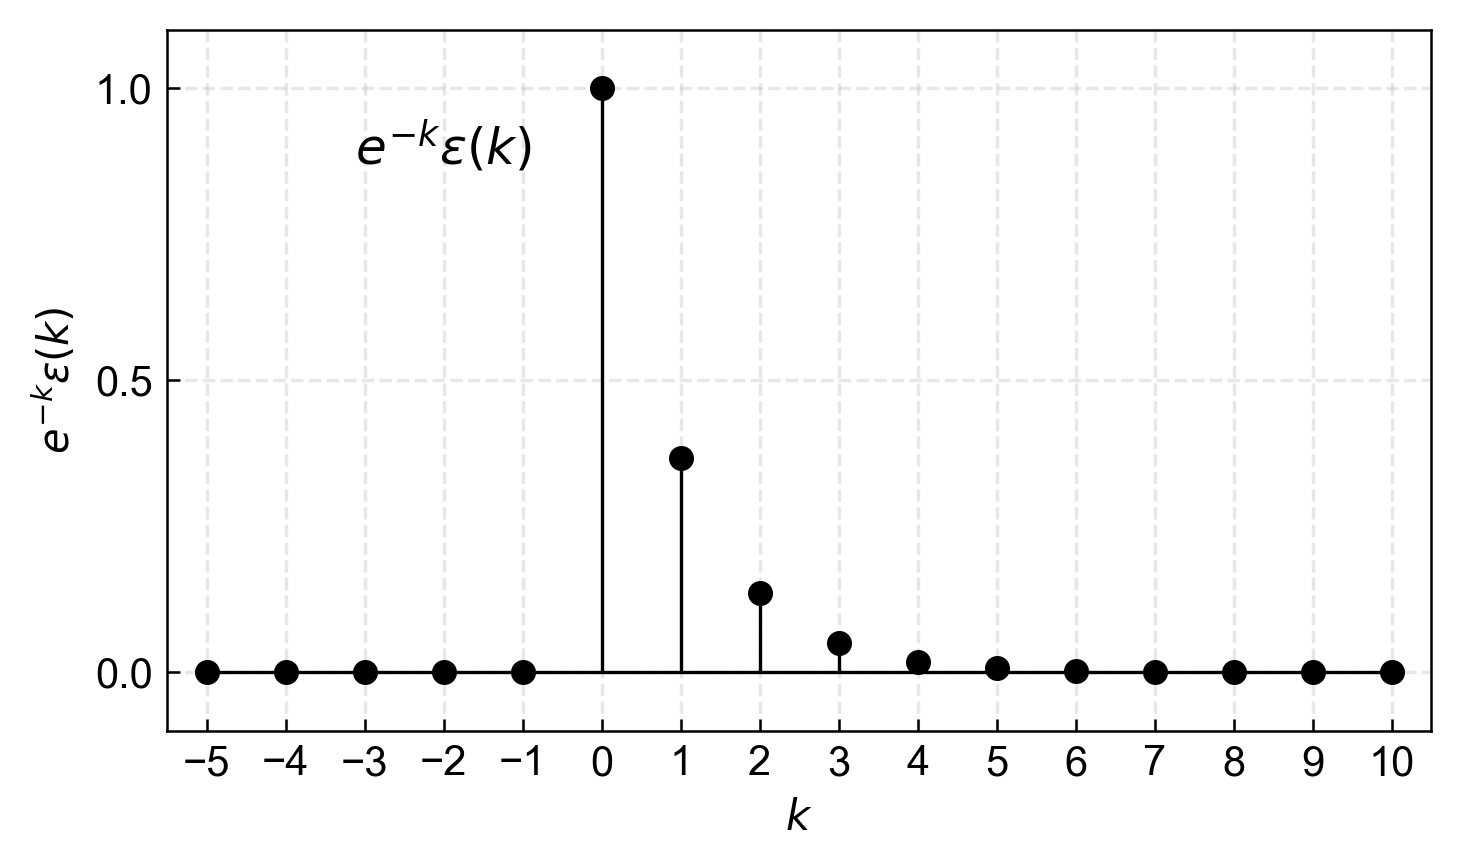
\includegraphics[width=0.5\textwidth]{img/笔记7.4.png}
\caption{单边指数序列}
\end{figure}

单边余弦序列
$$
\cos (\beta k) \varepsilon(k)
$$
\begin{figure}[H]
\centering
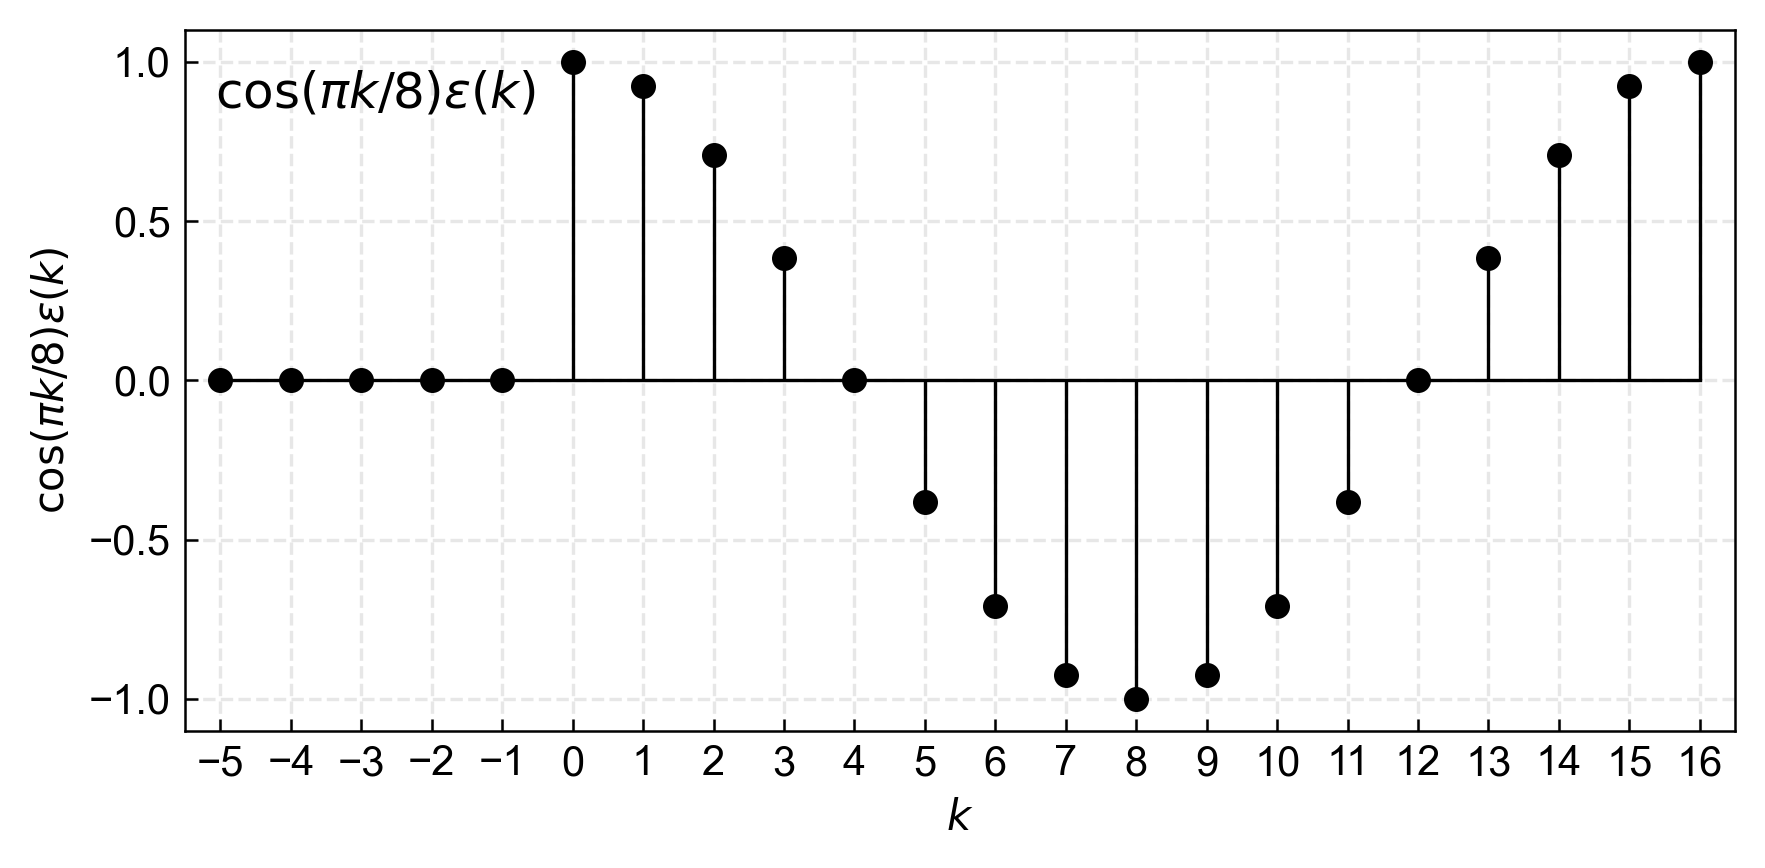
\includegraphics[width=0.5\textwidth]{img/笔记7.5.png}
\caption{单边余弦序列}
\end{figure}

\subsection{取样信号}

取样信号利用取样器（开关）实现。取样信号可看作原函数$f(t)$与开关函数$s(t)$的乘积。

$$
f_{S}(t)=f(t) s(t)
$$

对应频域关系为：
$$
f_S(t) \leftrightarrow \frac{1}{2\pi} F(j\omega) * S(j\omega)
$$
其中开关函数$s(t)$ 的取样间隔为$T_{S}$，$f_{S}=1 / T_{S}$称为取样频率。

\subsubsection{理想取样信号}

理想开关函数为周期冲激序列，对应的理想取样信号也称为冲激取样信号。

傅里叶变换对：
$$
f(t) \leftrightarrow F(j\omega),\quad \delta_{T_{S}}(t) \leftrightarrow \omega_{S} \delta_{\omega_{S}}(\omega)
$$

理想取样信号的时域表达式：
$$
f_{\delta}(t)=f(t) \delta_{T_{S}}(t) \leftrightarrow \frac{1}{2\pi} F(j\omega) * \omega_S \delta_{\omega_S}(\omega)
= \frac{1}{T_S} F(j\omega) * \delta_{\omega_S}(\omega)
$$

取样角频率定义：
$$
\omega_{S}=\frac{2 \pi}{T_{S}}
$$

\begin{figure}[H]
\centering
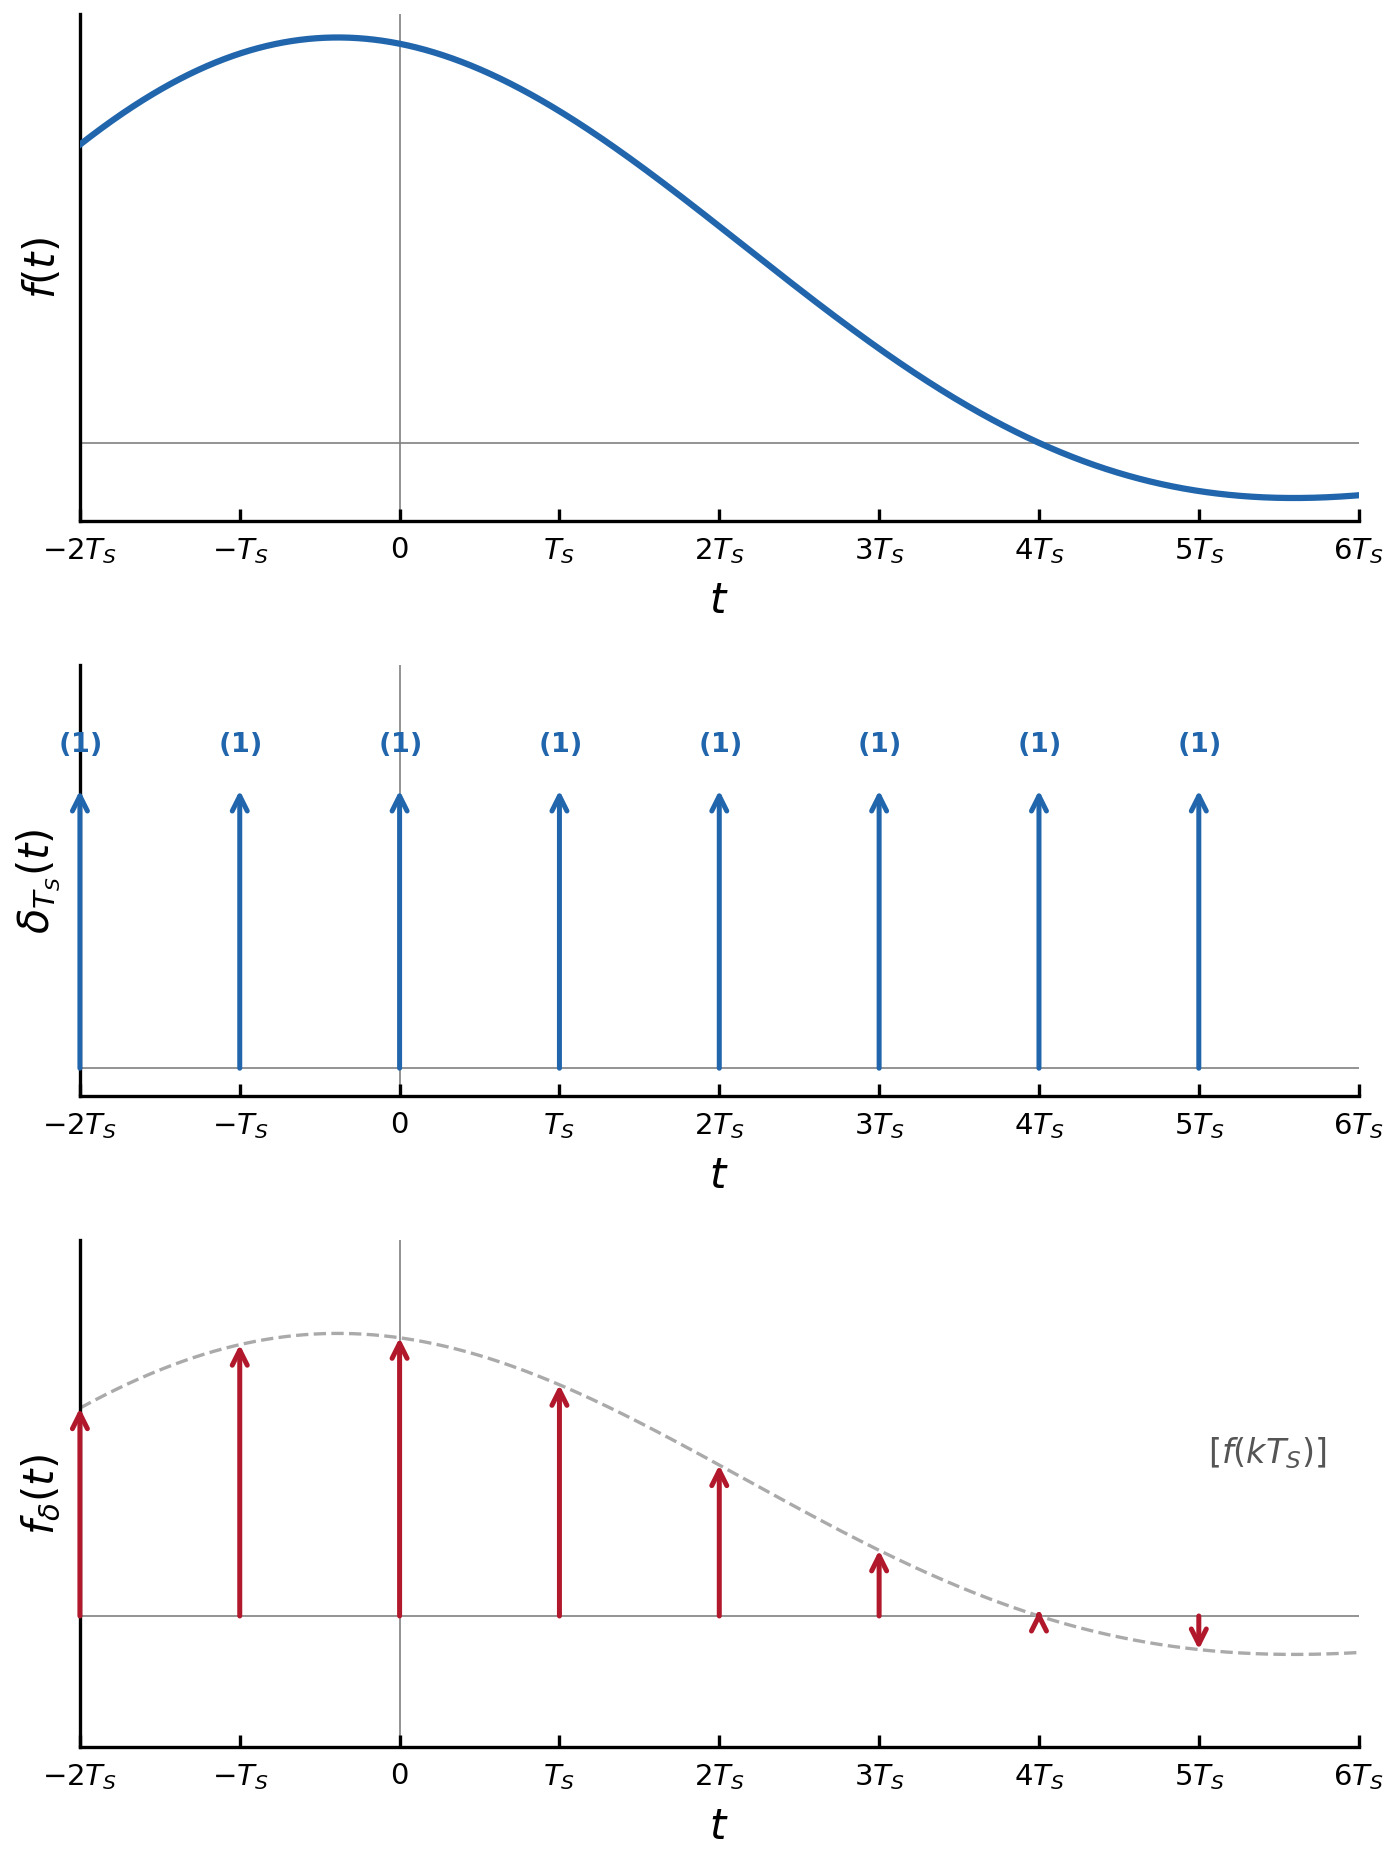
\includegraphics[width=0.5\textwidth]{img/笔记7.6.png}
\caption{理想取样信号}
\end{figure}

\subsubsection{理想取样信号的频谱特性}

理想取样信号的频谱是原函数频谱的周期延拓，周期为$\omega_{S}=2 \pi / T_{S}$，具体特性如下：
\begin{itemize}
    \item 各周期内的频谱形状与原信号频谱$F(j\omega)$ 相同
    \item 频谱幅度整体乘上因子$1 / T_{S}$
    \item 相邻周期频谱的间隔为$\omega_{S}$
\end{itemize}

理想取样信号的频谱展开式：
$$
F_\delta(j\omega) = \frac{1}{T_S} \sum_{k=-\infty}^{\infty} F\left( j\left(\omega - k\omega_S\right) \right)
$$

\begin{figure}[H]
\centering
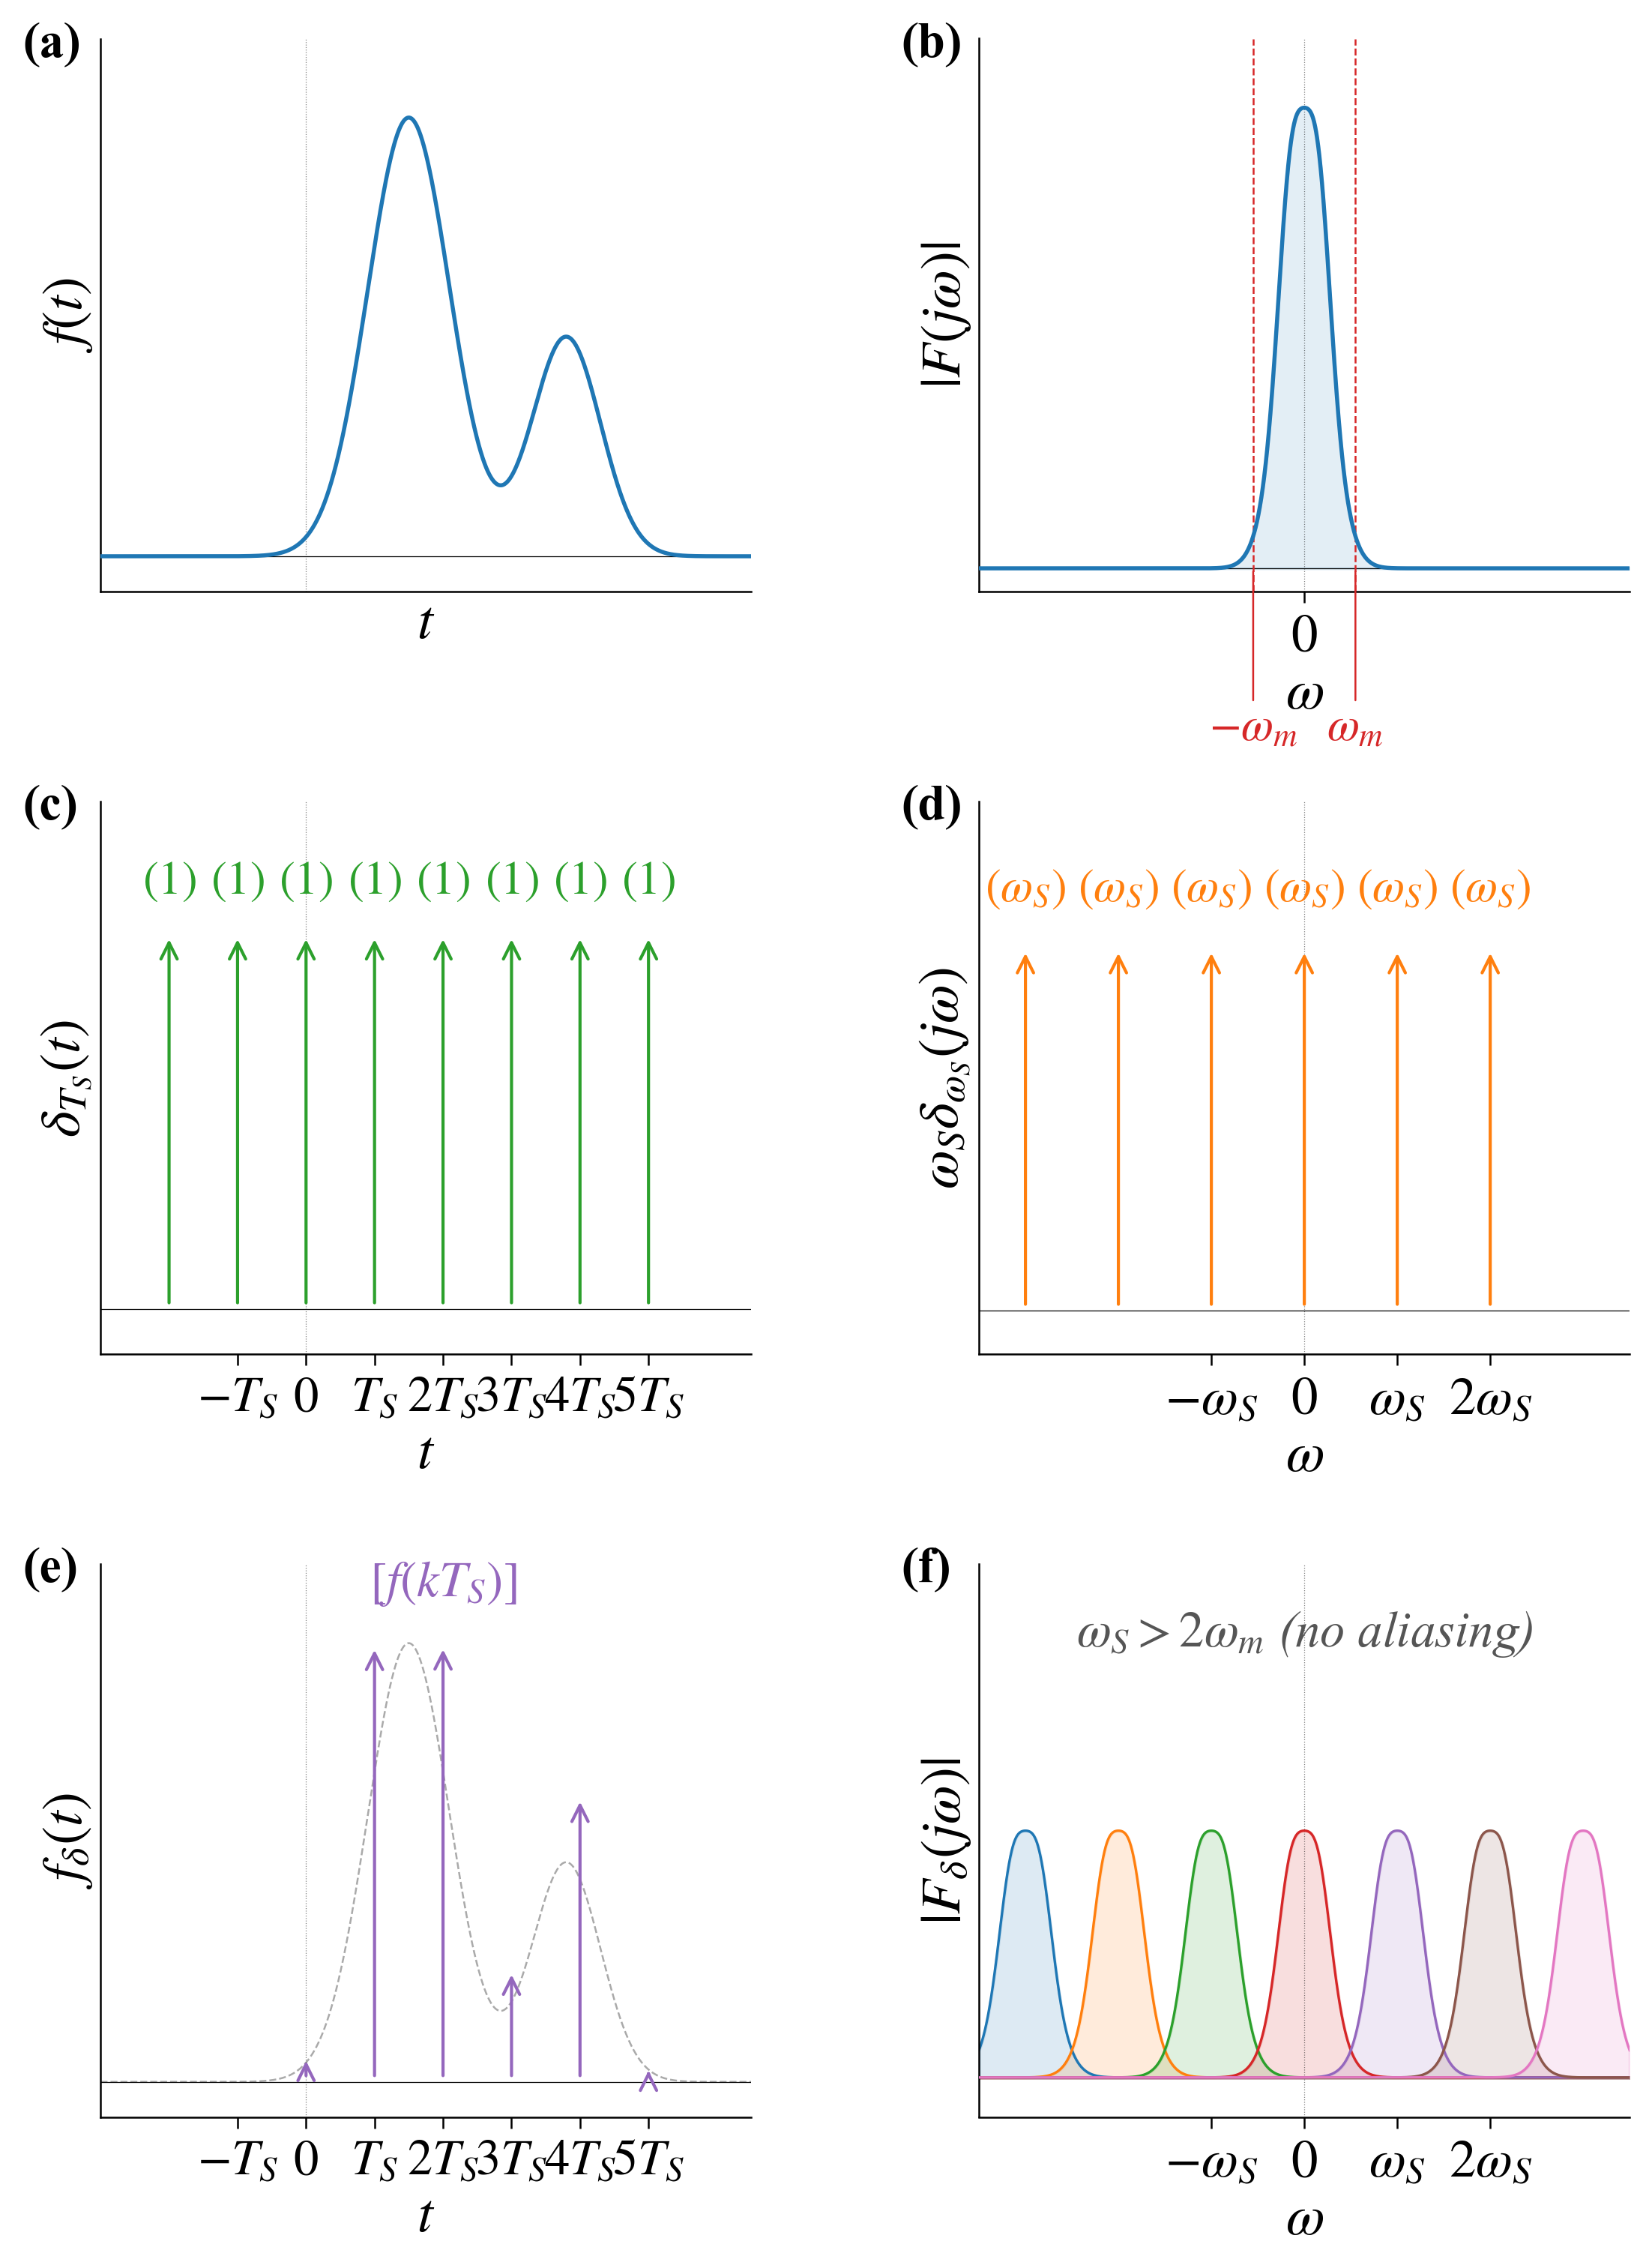
\includegraphics[width=0.5\textwidth]{img/笔记7.7.png}
\caption{理想取样信号频谱}
\end{figure}

\subsection{信号的重建}

理想取样信号的频谱中，包含频率平移量为零的基带分量，其与原信号频谱形状相同，幅度为$\dfrac{1}{T_S}$。

将理想取样信号通过截止频率为$\dfrac{\omega_{S}}{2}$、通带内幅度为$T_S$、相位为零的理想低通滤波器，即可重建原信号。

\subsubsection{信号重建的必要条件}
要实现无混叠的信号重建，取样信号的频谱中两相邻周期的部分不能重叠，需满足以下条件：
\begin{enumerate}
    \item 原信号 $F(j\omega)$ 为频带有限信号，即$|\omega| \leq \omega_{m}$
    \item 取样角频率大于或等于信号最高角频率的2倍：
    $$
    \omega_{S} \geq 2 \omega_{m}
    $$
\end{enumerate}

当理想低通滤波器的截止频率满足
$$
\omega_{m} \leq \omega_{c} \leq \omega_{s}-\omega_{m}
$$
时，理想低通的输出端可以恢复出原信号。

相关定义：
\begin{itemize}
    \item Shannon取样频率（Nyquist取样频率）：$2 \omega_{m}$ 或 $2 f_{m}$
    \item Shannon取样间隔（Nyquist取样间隔）：$1 / 2 f_{m}$ 或 $\pi / \omega_{m}$
\end{itemize}

\subsubsection{Shannon取样定理}
一个在频谱中不包含大于频率$f_{m}$ 的分量的有限频带信号，由对该信号以不大于$1/(2f_m)$ 的时间间隔进行取样的取样值唯一确定。当这样的信号通过截止频率满足$\omega_{m} \leq \omega_{c} \leq \omega_{S}-\omega_{m}$ 的理想低通滤波器后，可以将原信号完全重建。

$$
\omega_{s} \geq 2 \omega_{m}
$$
$$
T_{s} \leq \frac{1}{2 f_{m}}
$$
$$
f_{m}=\frac{\omega_{m}}{2 \pi}
$$
$$
\omega_{s}=\frac{2 \pi}{T_{s}}
$$

\section{LTI离散时间系统的描述和模拟}

\subsection{LTI离散时间系统}

\begin{itemize}
    \item 线性特性
    $$
    C_1e_1(k)+C_2e_2(k) \rightarrow \boxed{\text{系统}} \rightarrow C_1r_1(k)+C_2r_2(k)
    $$
    
    \item 移不变特性
    $$
    e(k-N) \rightarrow \boxed{\text{系统}} \rightarrow r(k-N)
    $$
    
    \item 线性移不变特性
    $$
    C_1e_1(k-M)+C_2e_2(k-N) \rightarrow \boxed{\text{系统}} \rightarrow C_1r_1(k-M)+C_2r_2(k-N)
    $$
\end{itemize}


\subsection{差分运算}

$f(t)$的取样信号$f(kT)$，简写为$f(k)$。

微分运算
$$
\frac{\mathrm{d}f(t)}{\mathrm{d} t}=\lim_{T \to 0}\frac{f(kT+T)-f(kT)}{T}
$$
差分运算

\begin{itemize}
    \item 一阶前向差分
    $$
    \frac{\Delta f(K)}{\Delta k}=\frac{f(k+1)-f(k)}{(k+1)-k}
    $$
    
    \item 一阶后向差分
    $$
    \frac{\nabla f(K)}{\nabla k}=\frac{f(k)-f(k-1)}{k-(k-1)}
    $$
\end{itemize}

$f(k+1)$和$f(k-1)$称为$f(k)$的移位序列。

\subsection{输入输出方程一般形式：n阶常系数差分方程}

$$
r(k+n)+a_{n-1}r(k+n-1)+\dots+a_1 r(k+1)+a_0 r(k)
= b_m e(k+m)+b_{m-1} e(k+m-1)+\dots+b_1 e(k+1)+b_0 e(k)
$$

差分方程包含离散变量及其增序或减序函数，描述离散序列中相邻几个数据点之间的数学关系。

差分方程的阶数等于自变量最高和最低移序量之差。

对比LTI连续时间系统的数学模型 —— n阶微分方程：

$$
r^{(n)} + a_{n-1} r^{(n-1)} + \dots + a_1 r' + a_0 r
= b_m e^{(m)} + b_{m-1} e^{(m-1)} + \dots + b_1 e' + b_0 e
$$

离散与连续系统的对应关系：
$$
r^{(n)} \to r(k+n)
$$

\subsection{移序算子}

移序算子$S$
$$
S[r(k)]=r(k+1)
$$

n阶差分方程的算子表示：
$$
\left(S^{n}+a_{n-1} S^{n-1}+\dots+a_{1} S+a_{0}\right) r(k)
$$

对比LTI连续时间系统的算子方程：
$$
\left(p^{n}+a_{n-1} p^{n-1}+\dots+a_{1} p+a_{0}\right) r(t)
$$

$$
H(p)=\frac{N(p)}{D(p)}
$$

\subsection{差分方程数值解法}

差分方程本质上是递推的代数方程，若已知初始条件和激励，利用迭代法可求得其数值解。

一阶常系数差分方程：
$$
r(k+1)+2 r(k)=e(k),\quad r(0)=1,\quad e(k)=2^{k} \varepsilon(k)
$$

这是前向差分方程，已知 $r(k)$、$e(k)$，可推出 $r(k+1)$ 及 $r(k+2)$、$r(k+3)$……

$$
\begin{aligned}
r(1)&=e(0)-2 r(0)=-1 \\
r(2)&=e(1)-2 r(1)=4 \\
r(3)&=e(2)-2 r(2)=-4
\end{aligned}
$$

一般无法得到解析解。

\section{LTI离散时间系统的零输入响应}

\subsection{零输入响应}

零输入响应即激励 $e(k)=0$ 时，齐次差分方程的解。

n阶齐次差分方程的一般形式：
$$
r(k+n)+a_{n-1} r(k+n-1)+\dots+a_{1} r(k+1)+a_{0} r(k)=0
$$

用移位算子 $S$ 可表示为：
$$
\left[S^{n}+a_{n-1} S^{n-1}+\dots+a_{1} S+a_{0}\right] r(k)=0
$$

令特征多项式 $D(S)=0$，n阶系统对应 $n$ 个初始条件 $r(0),r(1),\dots,r(n-1)$。求解特征方程得到特征根 $\gamma_1,\gamma_2,\dots$ 后，按根的类型构造解的形式：
\begin{itemize}
    \item 单根 $\gamma_i$ 对应的解分量：$r_i(k)=C_i \gamma_i^{k}$
    \item $p$ 重根 $\gamma_i$ 对应的解分量：$r_i(k)=\left(b_{1}+b_{2} k+\dots+b_{p} k^{p-1}\right) \gamma_{i}^{k}$
\end{itemize}

与连续系统对比：连续系统中单根对应解为 $r_i(t)=C_i e^{\lambda_i t}$，$p$ 重根对应解为
$$
r_i(t)=\left(b_{1}+b_{2} t+\dots+b_{p} t^{p-1}\right) e^{\lambda_i t}
$$

\subsection{一阶系统零输入响应}

一阶系统零输入响应可通过迭代法推导，一阶齐次差分方程为：
$$
r(k+1)+a_{0} r(k)=0
$$

特征多项式 $D(S)=S+a_{0}$，特征根 $\gamma=-a_0$。

迭代过程如下：
$$
r(1)=-a_{0} r(0)
$$
$$
r(2)=-a_{0} r(1)=\left(-a_{0}\right)^{2} r(0)
$$
$$
r(3)=-a_{0} r(2)=\left(-a_{0}\right)^{3} r(0)
$$
……

归纳得到通解形式：
$$
r(k)=C \gamma^{k}
$$

代入初始条件 $k=0$，得 $C=r(0)$，因此一阶系统零输入响应为：
$$
r(k)=\left(-a_{0}\right)^{k} r(0)
$$

\section{单位函数响应}

系统对单位样值序列$\delta(k)$的零状态响应，称单位函数响应，表示为$h(k)$。

令$e(k)=\delta(k)$，求解差分方程
$$
\left(S^{n}+a_{n-1} S^{n-1}+\dots+a_{1} S+a_{0}\right) h(k)=\left(b_mS^{m}+b_{m-1} S^{m-1}+\dots+b_{1}S+b_{0}\right) \delta(k)
$$

从转移算子求解，利用部分分式法及下表
$$
H(S)=\frac{N(S)}{D(S)}=\sum H_{i}(S) \Rightarrow h(k)=\sum h_{i}(k)
$$

转移算子对应的单位函数响应见表：

\begin{table}[H]
\centering
\begin{tabular}{c|c}
\hline
\textbf{转移算子 $H(S)$} & \textbf{单位函数响应 $h(k)$} \\
\hline
1 & $\delta(k)$ \\
\hline
$\dfrac{1}{S-\gamma}$ & $\gamma^{k-1} \varepsilon(k-1)$ \\
\hline
$\dfrac{S}{S-\gamma}$ & $\gamma^k \varepsilon(k)$ \\
\hline
$\dfrac{S}{(S-\gamma)^2}$ & $k\gamma^k \varepsilon(k)$ \\
\hline
$\dfrac{S}{(S-\gamma)^p}$ & $\dfrac{k(k-1)\cdots(k-p+2)}{(p-1)!}\gamma^{k-p+1}\varepsilon(k)$ \\
\hline
\end{tabular}
\end{table}

\subsection{n阶系统单位函数响应一般形式}
系统转移算子通式：
$$
H(S)=\frac{b_{m} S^{m}+b_{m-1} S^{m-1}+\dots+b_{1} S+b_{0}}{S^{n}+a_{n-1} S^{n-1}+\dots+a_{1} S+a_{0}}
$$

按分子分母阶次分情况：

\begin{enumerate}
    \item $m<n,\ b_{0}=0$
    $$
    H(S)=\sum \frac{A_{i}}{S-\gamma_{i}}
    $$
    $$
    h(k)=\sum A_{i} \gamma_{i}^{k-1} \varepsilon(k-1)
    $$
    
    \item $m=n,\ b_{0} \neq 0$
    \begin{itemize}
        \item 形式一：
        $$
        H(S)=S\left[\sum \frac{A_{i}}{S-\gamma_{i}}\right]
        $$
        $$
        h(k)=\sum A_{i} \gamma_{i}^{k} \varepsilon(k)
        $$
        \item 形式二：
        $$
        H(S)=1+\sum \frac{A_{i}}{S-\gamma_{i}}
        $$
        $$
        h(k)=\delta(k)+\sum A_{i} \gamma_{i}^{k-1} \varepsilon(k-1)
        $$
    \end{itemize}
    
    \item $m<n,\ b_{0} \neq 0$
    $$
    H(S)=\sum \frac{A_{i}}{S-\gamma_{i}}
    $$
    $$
    h(k)=\sum A_{i} \gamma_{i}^{k-1} \varepsilon(k-1)
    $$
\end{enumerate}

\section{卷积和}

\section{LTI离散时间系统的零状态响应}

利用卷积和求系统零状态响应

离散序列的冲激分解：
$$
e(k)=\sum_{j=0}^{k} e(j) \delta(k-j)=e(k) * \delta(k)
$$

离散系统零状态响应：
$$
r_{zs}(k)=\sum_{j=0}^{k} e(j) h(k-j)=e(k) * h(k)
$$

对比连续时间系统零状态响应：
$$
e(t)=\int_{0}^{t} e(\tau) \delta(t-\tau) \mathrm{d}\tau=e(t) * \delta(t)
$$
$$
r_{zs}(t)=\int_{0}^{t} e(\tau) h(t-\tau) \mathrm{d}\tau=e(t) * h(t)
$$

\subsection{离散时间系统全响应}

全响应分解为零输入响应与零状态响应之和：
$$
\begin{aligned}
r(k) & =r_{zi}(k)+r_{zs}(k) \\
& =\sum C_{i} \gamma_{i}^{k} \varepsilon(k)+e(k) * h(k)
\end{aligned}
$$

对比连续时间系统全响应：
$$
\begin{aligned}
r(t) & =r_{zi}(t)+r_{zs}(t) \\
& =\sum C_{i} e^{\lambda_{i} t} \varepsilon(t)+e(t) * h(t)
\end{aligned}
$$

离散与连续系统的对应关系：
$$
\begin{aligned}
t&=k T_{S} \\
e^{\lambda t} &\to \gamma^{k} \\
e^{\lambda T_{S}} &\to \gamma
\end{aligned}
$$

\section{离散时间系统作业}

\subsection{例题1}

\begin{problem}
已知一阶线性微分方程
$$
\frac{\mathrm{d}}{\mathrm{d}t} r(t) + a r(t) = b e(t)
$$
取离散时刻$t = kT$（$k$为整数，$T$为采样步长），当$T \to 0$时，用向前差商
$$
\frac{\mathrm{d}}{\mathrm{d}t} r(t) \approx \frac{r(kT + T) - r(kT)}{T}
$$
近似替代导数项，将该微分方程转化为近似的差分方程。
\end{problem}

\begin{solution}
记离散序列$r(k) = r(kT)$，$e(k) = e(kT)$，将向前差商代入原微分方程，得到：
$$
\frac{r(k+1) - r(k)}{T} + a r(k) = b e(k)
$$

等式两边同乘$T$并整理项：
$$
r(k+1) - r(k) + aT \cdot r(k) = bT \cdot e(k)
$$

合并同类项后，得到标准一阶线性差分方程：
$$
r(k+1) + (aT - 1) r(k) = bT e(k)
$$
\end{solution}

\subsection{零输入响应练习1}

\begin{problem}
已知差分方程 $r(k+2)+4r(k+1)+4r(k)=0$，初始条件 $r(0)=2$，$r(1)=2$，求零输入响应。
\end{problem}

\begin{solution}
特征方程：

$$
D(S)=S^{2}+4S+4=(S+2)^{2}=0
$$

特征根 $\gamma_{1,2}=-2$

零输入响应形式：

$$
y_{zi}(k)=\left(C_{1}+C_{2}k\right)(-2)^{k}\varepsilon(k)
$$


代入初始条件求解系数：

$$
\begin{cases}
r(0)=C_{1}=2 \\
r(1)=\left(C_{1}+C_{2}\right)(-2)=2
\end{cases}
\Rightarrow
\begin{cases}
C_{1}=2 \\
C_{2}=-3
\end{cases}
$$


最终零输入响应：

$$
y_{zi}(k)=(2-3k)(-2)^{k}\varepsilon(k)
$$
\end{solution}

\subsection{零输入响应练习2}

\begin{problem}
已知差分方程 $r(k+3)+6r(k+2)+12r(k+1)+8r(k)=0$，初始条件 $r(0)=1$，$r(1)=1$，$r(2)=0$，求零输入响应。
\end{problem}

\begin{solution}
特征方程：

$$
D(S)=S^{3}+6S^{2}+12S+8=(S+2)^{3}=0
$$

特征根 $\gamma_{1,2,3}=-2$

零输入响应形式：

$$
y_{zi}(k)=\left(C_{1}+C_{2}k+C_{3}k^{2}\right)(-2)^{k}\varepsilon(k)
$$


代入初始条件：

$$
r(0)=C_{1}=1
$$


$$
r(1)=\left(C_{1}+C_{2}+C_{3}\right)(-2)=1
$$


$$
r(2)=\left(C_{1}+2C_{2}+4C_{3}\right)(-2)^{2}=0
$$
\end{solution}

\subsection{零输入响应练习3}

\begin{problem}
已知差分方程 $r(k+4)-2r(k+3)+2r(k+2)-2r(k+1)+r(k)=0$，初始条件 $r(1)=1$，$r(2)=0$，$r(3)=1$，$r(5)=1$，求零输入响应。
\end{problem}

\begin{solution}
特征方程：

$$
D(S)=S^{4}-2S^{3}+2S^{2}-2S+1=(S-1)^{2}\left(S^{2}+1\right)=0
$$

特征根 $\gamma_{1,2}=1$，$\gamma_{3,4}=\pm j$

零输入响应复指数形式：

$$
y_{zi}(k)=\left(C_{1}+C_{2}k\right)1^{k}+C_{3}j^{k}+C_{4}(-j)^{k}
$$


或实函数形式：

$$
y_{zi}(k)=\left(C_{1}+C_{2}k\right)1^{k}+C_{3}\cos\frac{k\pi}{2}+C_{4}\sin\frac{k\pi}{2}
$$


最终零输入响应：

$$
y_{zi}(k)=1+\cos\frac{k\pi}{2}
$$
\end{solution}

\subsection{单位函数响应练习1}

\begin{problem}
一阶系统，差分方程：$h(k+1)-\gamma h(k)=\delta(k)$
\end{problem}

\begin{solution}
转移算子：
$$
H(S)=\frac{1}{S-\gamma}
$$

初始值递推计算：
$$
\begin{aligned}
h(0)&=\delta(-1)+\gamma h(-1)=0 \\
h(1)&=\delta(0)+\gamma h(0)=1=\gamma^{0} \\
h(2)&=\delta(1)+\gamma h(1)=\gamma h(1)=\gamma \\
\end{aligned}
$$

通用递推推导：
$$
\begin{aligned}
h(k) & =\delta(k-1)+\gamma h(k-1) \\
& =\gamma h(k-1) \\
& =\gamma\left[\gamma h(k-2)\right] \\
& =\gamma^{k-1} h(1)
\end{aligned}
$$

最终单位函数响应：
$$
h(k)=\gamma^{k-1} \varepsilon(k-1)
$$

其中单位序列定义：
$$\delta(k)=
\begin{cases}
1 & k=0 \\
0 & k \neq 0
\end{cases}$$
\end{solution}

\subsection{单位函数响应练习2}

\begin{problem}
差分方程：$r(k+1)-\gamma r(k)=e(k+1)$
\end{problem}

\begin{solution}
转移算子拆分：
$$
H(S)=\frac{r(k)}{e(k)}=\frac{S}{S-\gamma}=1+\frac{\gamma}{S-\gamma}
$$

单位函数响应推导：
$$
\begin{aligned}
h(k) & =\delta(k)+\gamma \cdot \gamma^{k-1} \varepsilon(k-1) \\
& =\delta(k)+\gamma^{k}\left[\varepsilon(k)-\delta(k)\right]=\gamma^{k} \varepsilon(k)
\end{aligned}
$$

结论：当系统转移算子满足 $m=n$ 且比值常数为1时，输出响应中包含一个输入激励的直通分量。
\end{solution}

\subsection{单位函数响应练习3}

\begin{problem}
已知差分方程 $r(k+2)+2 r(k+1)-3 r(k)=e(k+1)+2 e(k)$，求单位函数响应
\end{problem}

\begin{solution}
对转移算子做部分分式展开：
$$
H(S)=\frac{S+2}{S^{2}+2 S-3}=\frac{3 / 4}{S-1}+\frac{1 / 4}{S+3}
$$

单位函数响应：
$$
h(k)=\frac{3}{4} \cdot 1^{k-1} \varepsilon(k-1)+\frac{1}{4}(-3)^{k-1} \varepsilon(k-1)
$$
\end{solution}

\subsection{单位函数响应练习4}

\begin{problem}
已知差分方程 $r(k+2)-2 \gamma r(k+1)+\gamma^{2} r(k)=e(k)$，求单位函数响应
\end{problem}

\begin{solution}
对转移算子做变形拆分：
$$
H(S)=\frac{1}{(S-\gamma)^{2}}=\left[\frac{S}{(S-\gamma)^{2}}-\frac{1}{S-\gamma}\right] \frac{1}{\gamma}
$$

单位函数响应推导：
$$
\begin{aligned}
h(k) & =\left[k \gamma^{k-1} \varepsilon(k)-\gamma^{k-1} \varepsilon(k-1)\right] \gamma^{-1} \\
& =(k-1) \gamma^{k-2} \varepsilon(k-1)
\end{aligned}
$$
\end{solution}

\subsection{离散时间系统综合练习1}

\begin{problem}
已知系统差分方程：$r(k+2)-3 r(k+1)+2 r(k)=e(k+1)-3 e(k)$
激励 $e(k)=\varepsilon(k)$，零输入初始条件 $r_{zi}(0)=1,\ r_{zi}(1)=0$，求系统全响应。
\end{problem}

\begin{solution}
\textbf{单位函数响应}
系统转移算子及部分分式展开：
$$
H(S)=\frac{r(k)}{e(k)}=\frac{S-3}{S^{2}-3 S+2}=\frac{2}{S-1}+\frac{-1}{S-2}
$$

单位函数响应推导：
$$
\begin{aligned}
h(k) & =\left[2(1)^{k-1}-(2)^{k-1}\right] \varepsilon(k-1) \\
& =\left[2(1)^{k-1}-(2)^{k-1}\right][\varepsilon(k)-\delta(k)] \\
& =\left[2-\frac{1}{2} 2^{k}\right] \varepsilon(k)-\frac{3}{2} \delta(k)
\end{aligned}
$$

\textbf{零输入响应}
零输入响应通式：
$$r_{zi}(k)=\left[C_{1}(1)^{k}+C_{2}(2)^{k}\right] \varepsilon(k)$$

代入初始条件求解系数：
$$
\left\{
\begin{array}{c}
r_{zi}(0)=C_{1}+C_{2}=1 \\
r_{zi}(1)=C_{1}+2 C_{2}=0
\end{array}
\right.
\Rightarrow
\left\{
\begin{array}{c}
C_{1}=2 \\
C_{2}=-1
\end{array}
\right.
$$

得零输入响应：
$$
r_{zi}(k)=\left[2-2^{k}\right] \varepsilon(k)
$$

\textbf{零状态响应}
零状态响应由卷积和计算：$r_{zs}(k)=e(k) * h(k)$

用到卷积公式：
$$
\gamma^{k} \varepsilon(k) * \varepsilon(k)=\frac{1-\gamma^{k+1}}{1-\gamma} \varepsilon(k)
$$

代入 $e(k)=\varepsilon(k)$ 与 $h(k)$ 计算：
$$
\begin{aligned}
r_{zs}(k) & =\varepsilon(k) *\left[2-\frac{1}{2} 2^{k}\right] \varepsilon(k)-\varepsilon(k) * \frac{3}{2} \delta(k) \\
& =\left[2 k+\frac{1}{2}\left(1-2^{k+1}\right)\right] \varepsilon(k)-\frac{3}{2} \varepsilon(k) \\
& =\left[2 k-2^{k}-1\right] \varepsilon(k)
\end{aligned}
$$

\textbf{全响应}
全响应为零输入响应与零状态响应之和：
$$
\begin{aligned}
r(k) & =r_{zi}(k)+r_{zs}(k) \\
& =\left[2-2^{k}\right] \varepsilon(k)+\left[2 k-2^{k}-1\right] \varepsilon(k) \\
& =\left[2 k-2^{k+1}+1\right] \varepsilon(k)
\end{aligned}
$$
\end{solution}

\subsection{离散时间系统综合练习2}

\begin{problem}
已知系统差分方程：$r(k+2)+3 r(k+1)+2 r(k)=e(k+2)$
激励 $e(k)=2^{k} \varepsilon(k)$，初始条件 $r(-1)=0$，$r(-2)=0.5$，求系统零输入响应、零状态响应、全响应。
\end{problem}

\begin{solution}
\textbf{零输入响应}
零输入响应满足齐次差分方程：
$$
r_{zi}(k+2)+3 r_{zi}(k+1)+2 r_{zi}(k)=0
$$

初始条件分解：零输入响应继承系统初始条件，零状态响应在负时刻取值为0
$$
r_{zi}(-1)=r(-1)=0,\quad r_{zi}(-2)=r(-2)=0.5
$$
$$
r_{zs}(-1)=0,\quad r_{zs}(-2)=0
$$

代入齐次方程递推$k \geq 0$的初始值：
$$
r_{zi}(0)+3 r_{zi}(-1)+2 r_{zi}(-2)=0 \Rightarrow r_{zi}(0)=-1
$$
$$
r_{zi}(1)+3 r_{zi}(0)+2 r_{zi}(-1)=0 \Rightarrow r_{zi}(1)=3
$$

系统特征根为两个单根：$\gamma_{1}=-1,\ \gamma_{2}=-2$，零输入响应通式为
$$
r_{zi}(k)=\left[C_{1}(-1)^{k}+C_{2}(-2)^{k}\right] \varepsilon(k)
$$

代入初始值求解系数：
$$
\left\{
\begin{array}{c}
r_{zi}(0) = -1 \\
r_{zi}(1) = 3
\end{array}
\right.
\Rightarrow
\left\{
\begin{array}{c}
C_{1}=1 \\
C_{2}=-2
\end{array}
\right.
$$

最终零输入响应：
$$
r_{zi}(k)=\left[(-1)^{k}-2(-2)^{k}\right] \varepsilon(k)
$$

\textbf{零状态响应}

系统转移算子及部分分式展开：
$$
H(S)=\frac{S^{2}}{S^{2}+3 S+2}=\frac{-S}{S+1}+\frac{2 S}{S+2}
$$

单位函数响应：
$$
h(k)=\left[-(-1)^{k}+2(-2)^{k}\right] \varepsilon(k)
$$

零状态响应由卷积和计算 $r_{zs}(k)=e(k) * h(k)$，代入激励与单位响应：
$$
\begin{aligned}
r_{zs}(k) &=2^{k} \varepsilon(k) *\left[-(-1)^{k}+2(-2)^{k}\right] \varepsilon(k) \\
&=-\frac{2^{k+1}-(-1)^{k+1}}{3} \varepsilon(k)+2 \cdot\frac{2^{k+1}-(-2)^{k+1}}{4} \varepsilon(k) \\
&=\left[\frac{1}{3} 2^{k}-\frac{1}{3}(-1)^{k}+(-2)^{k}\right] \varepsilon(k)
\end{aligned}
$$
对应零状态初始值：$\begin{cases} r_{zs}(0)=1 \\ r_{zs}(1)=-1 \end{cases}$

\textbf{全响应}
全响应为零输入响应与零状态响应之和：
$$
\begin{aligned}
r(k) &=r_{zi}(k)+r_{zs}(k) \\
&=\left[\frac{1}{3} 2^{k}+\frac{2}{3}(-1)^{k}-(-2)^{k}\right] \varepsilon(k)
\end{aligned}
$$
对应全响应初始值：$\begin{cases} r(0)=0 \\ r(1)=2 \end{cases}$
\end{solution}

\end{document}